\documentclass[11pt,]{article}
\usepackage[left=1in,top=1in,right=1in,bottom=1in]{geometry}
\newcommand*{\authorfont}{\fontfamily{phv}\selectfont}
\usepackage[]{mathpazo}


  \usepackage[T1]{fontenc}
  \usepackage[utf8]{inputenc}



\usepackage{abstract}
\renewcommand{\abstractname}{}    % clear the title
\renewcommand{\absnamepos}{empty} % originally center

\renewenvironment{abstract}
 {{%
    \setlength{\leftmargin}{0mm}
    \setlength{\rightmargin}{\leftmargin}%
  }%
  \relax}
 {\endlist}

\makeatletter
\def\@maketitle{%
  \newpage
%  \null
%  \vskip 2em%
%  \begin{center}%
  \let \footnote \thanks
    {\fontsize{18}{20}\selectfont\raggedright  \setlength{\parindent}{0pt} \@title \par}%
}
%\fi
\makeatother




\setcounter{secnumdepth}{3}

\usepackage{color}
\usepackage{fancyvrb}
\newcommand{\VerbBar}{|}
\newcommand{\VERB}{\Verb[commandchars=\\\{\}]}
\DefineVerbatimEnvironment{Highlighting}{Verbatim}{commandchars=\\\{\}}
% Add ',fontsize=\small' for more characters per line
\usepackage{framed}
\definecolor{shadecolor}{RGB}{248,248,248}
\newenvironment{Shaded}{\begin{snugshade}}{\end{snugshade}}
\newcommand{\KeywordTok}[1]{\textcolor[rgb]{0.13,0.29,0.53}{\textbf{#1}}}
\newcommand{\DataTypeTok}[1]{\textcolor[rgb]{0.13,0.29,0.53}{#1}}
\newcommand{\DecValTok}[1]{\textcolor[rgb]{0.00,0.00,0.81}{#1}}
\newcommand{\BaseNTok}[1]{\textcolor[rgb]{0.00,0.00,0.81}{#1}}
\newcommand{\FloatTok}[1]{\textcolor[rgb]{0.00,0.00,0.81}{#1}}
\newcommand{\ConstantTok}[1]{\textcolor[rgb]{0.00,0.00,0.00}{#1}}
\newcommand{\CharTok}[1]{\textcolor[rgb]{0.31,0.60,0.02}{#1}}
\newcommand{\SpecialCharTok}[1]{\textcolor[rgb]{0.00,0.00,0.00}{#1}}
\newcommand{\StringTok}[1]{\textcolor[rgb]{0.31,0.60,0.02}{#1}}
\newcommand{\VerbatimStringTok}[1]{\textcolor[rgb]{0.31,0.60,0.02}{#1}}
\newcommand{\SpecialStringTok}[1]{\textcolor[rgb]{0.31,0.60,0.02}{#1}}
\newcommand{\ImportTok}[1]{#1}
\newcommand{\CommentTok}[1]{\textcolor[rgb]{0.56,0.35,0.01}{\textit{#1}}}
\newcommand{\DocumentationTok}[1]{\textcolor[rgb]{0.56,0.35,0.01}{\textbf{\textit{#1}}}}
\newcommand{\AnnotationTok}[1]{\textcolor[rgb]{0.56,0.35,0.01}{\textbf{\textit{#1}}}}
\newcommand{\CommentVarTok}[1]{\textcolor[rgb]{0.56,0.35,0.01}{\textbf{\textit{#1}}}}
\newcommand{\OtherTok}[1]{\textcolor[rgb]{0.56,0.35,0.01}{#1}}
\newcommand{\FunctionTok}[1]{\textcolor[rgb]{0.00,0.00,0.00}{#1}}
\newcommand{\VariableTok}[1]{\textcolor[rgb]{0.00,0.00,0.00}{#1}}
\newcommand{\ControlFlowTok}[1]{\textcolor[rgb]{0.13,0.29,0.53}{\textbf{#1}}}
\newcommand{\OperatorTok}[1]{\textcolor[rgb]{0.81,0.36,0.00}{\textbf{#1}}}
\newcommand{\BuiltInTok}[1]{#1}
\newcommand{\ExtensionTok}[1]{#1}
\newcommand{\PreprocessorTok}[1]{\textcolor[rgb]{0.56,0.35,0.01}{\textit{#1}}}
\newcommand{\AttributeTok}[1]{\textcolor[rgb]{0.77,0.63,0.00}{#1}}
\newcommand{\RegionMarkerTok}[1]{#1}
\newcommand{\InformationTok}[1]{\textcolor[rgb]{0.56,0.35,0.01}{\textbf{\textit{#1}}}}
\newcommand{\WarningTok}[1]{\textcolor[rgb]{0.56,0.35,0.01}{\textbf{\textit{#1}}}}
\newcommand{\AlertTok}[1]{\textcolor[rgb]{0.94,0.16,0.16}{#1}}
\newcommand{\ErrorTok}[1]{\textcolor[rgb]{0.64,0.00,0.00}{\textbf{#1}}}
\newcommand{\NormalTok}[1]{#1}
\usepackage{longtable,booktabs}

\usepackage{graphicx,grffile}
\makeatletter
\def\maxwidth{\ifdim\Gin@nat@width>\linewidth\linewidth\else\Gin@nat@width\fi}
\def\maxheight{\ifdim\Gin@nat@height>\textheight\textheight\else\Gin@nat@height\fi}
\makeatother
% Scale images if necessary, so that they will not overflow the page
% margins by default, and it is still possible to overwrite the defaults
% using explicit options in \includegraphics[width, height, ...]{}
\setkeys{Gin}{width=\maxwidth,height=\maxheight,keepaspectratio}

\title{Asociación y abundancia relativa de especies de la familia Rubiaceae en
la parcela permanente Isla Barro Colorado  }



\author{\Large J. Alberto Meléndez Juan\vspace{0.05in} \newline\normalsize\emph{Universidad Autónoma de Santo Domingo (UASD)}  }


\date{}

\usepackage{titlesec}

\titleformat*{\section}{\normalsize\bfseries}
\titleformat*{\subsection}{\normalsize\itshape}
\titleformat*{\subsubsection}{\normalsize\itshape}
\titleformat*{\paragraph}{\normalsize\itshape}
\titleformat*{\subparagraph}{\normalsize\itshape}

\titlespacing{\section}
{0pt}{36pt}{0pt}
\titlespacing{\subsection}
{0pt}{36pt}{0pt}
\titlespacing{\subsubsection}
{0pt}{36pt}{0pt}





\newtheorem{hypothesis}{Hypothesis}
\usepackage{setspace}

\makeatletter
\@ifpackageloaded{hyperref}{}{%
\ifxetex
  \PassOptionsToPackage{hyphens}{url}\usepackage[setpagesize=false, % page size defined by xetex
              unicode=false, % unicode breaks when used with xetex
              xetex]{hyperref}
\else
  \PassOptionsToPackage{hyphens}{url}\usepackage[unicode=true]{hyperref}
\fi
}

\@ifpackageloaded{color}{
    \PassOptionsToPackage{usenames,dvipsnames}{color}
}{%
    \usepackage[usenames,dvipsnames]{color}
}
\makeatother
\hypersetup{breaklinks=true,
            bookmarks=true,
            pdfauthor={J. Alberto Meléndez Juan (Universidad Autónoma de Santo Domingo (UASD))},
             pdfkeywords = {Especies dominantes, Diversidad, Rubiaceae},  
            pdftitle={Asociación y abundancia relativa de especies de la familia Rubiaceae en
la parcela permanente Isla Barro Colorado},
            colorlinks=true,
            citecolor=blue,
            urlcolor=blue,
            linkcolor=magenta,
            pdfborder={0 0 0}}
\urlstyle{same}  % don't use monospace font for urls

% set default figure placement to htbp
\makeatletter
\def\fps@figure{htbp}
\makeatother

\usepackage{amsmath}

\usepackage{pdflscape} \newcommand{\blandscape}{\begin{landscape}} \newcommand{\elandscape}{\end{landscape}} \usepackage{float} \floatplacement{figure}{H} \newcommand{\beginsupplement}{ \setcounter{table}{0} \renewcommand{\thetable}{S\arabic{table}} \setcounter{figure}{0} \renewcommand{\thefigure}{S\arabic{figure}} }


% add tightlist ----------
\providecommand{\tightlist}{%
\setlength{\itemsep}{0pt}\setlength{\parskip}{0pt}}

\begin{document}
	
% \pagenumbering{arabic}% resets `page` counter to 1 
%
% \maketitle

{% \usefont{T1}{pnc}{m}{n}
\setlength{\parindent}{0pt}
\thispagestyle{plain}
{\fontsize{18}{20}\selectfont\raggedright 
\maketitle  % title \par  

}

{
   \vskip 13.5pt\relax \normalsize\fontsize{11}{12} 
\textbf{\authorfont J. Alberto Meléndez Juan} \hskip 15pt \emph{\small Universidad Autónoma de Santo Domingo (UASD)}   

}

}








\begin{abstract}

    \hbox{\vrule height .2pt width 39.14pc}

    \vskip 8.5pt % \small 

\noindent \textbf{Resumen} El estudio del grado de ordenación y riqueza de las
comunidades de especies depende en gran medida de interacciónes entre
las distintas especies y su hábitat. En este trabajo se estudian los
patrones de asociación entre las especies de la familia Rubiaceae y como
varía la diversidad con respecto a las características del hábitat. Se
encontró que la comunidad presenta disparidad en la abundancia, con
especies muy dominantes y muchas otras pobremente representadas. Las
ocurrencias de especies como \emph{Psychotria horizontalis} y
\emph{Psychotria marginata} están asociadas con la cantidad de alumínio
y fósforo en el suelo. La especie \emph{Alseis blackiana} presenta
asociación con el contenido de los metales manganeso, hierro y cobre.
Los resultados sugieren que la especialización a ciertas condiciones
puede verse reflejada en la asociación al hábitat incluso en una escala
muy local. Más allá de su significado ecológico, la distribución de las
poblaciones de estas plantas tolerantes podría servir para indicar
ocurrencias anormales en la concentración de metales pesados en el
ambiente.


\vskip 8.5pt \noindent \emph{Keywords}: Especies dominantes, Diversidad, Rubiaceae \par

    \hbox{\vrule height .2pt width 39.14pc}



\end{abstract}


\vskip 6.5pt


\noindent  \section{Introducción}\label{introducciuxf3n}

Las comunidades vegetales de los bosques neotropicales ejemplifican la
diversidad y complejidad ecológica de la región tropical. El estudio
continuo de su riqueza y abundancia relativa permite identificar las
especies raras, las cuales son más vulnerables a los cambios en su
hábitat y por lo tanto propensas a extinguirse localmente (Volkov,
Banavar, Hubbell, \& Maritan, 2003). Adicionalmente, monitorear la
diversidad como propiedad de las comunidades vivientes resulta de suma
importancia para analizar el efecto que tiene la transformación de los
ecosistemas en las comunidades naturales. Claramente existe entonces la
necesidad de conocer como se encuentran asociadas las especies entre sí
dentro de las comunidades ecológicas para ayudar a comprender los
factores que inciden en su conservación (Moreno, 2001).

La familia Rubiaceae es un importante grupo de plantas vasculares de
distribución cosmopolita con una marcada diversidad en regiones
tropicales y subtropicales (Davis et al., 2009). Muchas de las especies
que componen esta familia se encuentran adaptadas a la vida en la
penúmbra, y prosperan bajo la sombra del dosel selvático. En estas
selvas tropicales, el grado de ordenación y riqueza de las comunidades
que componen el sotobosque, depende en gran medida de interacciónes
entre las distintas especies (Torres-Leite et al., 2019). También, este
grado de ordenación se asocia con factores ambientales de su hábitat, ya
que muchas de estas especies estan adaptadas a rangos elevados de ácidez
y otras condiciones específicas de los componentes del suelo, como la
concentración de distintos metales (Jansen, Robbrecht, Beeckman, \&
Smets, 2000).

Es preciso señalar que trabajos anteriores (Condit et al., 2002) sobre
el bosque tropical panameño y el grado de reemplazo entre especies de
distintas comunidades o diversidad beta, sugieren que la disimilaridad
tiende a aumentar en función de la distancia a la cual se encuentran
separadas en el espacio. Sin embargo, estos trabajos no restan
importancia a la variabilidad del hábitat y se toman en cuenta en este
estudio, ya que un acercamiento inicial a los datos de abundancia de las
distintas especies de Rubiaceae en Barro Colorado arrojó indicios de
posibles patrones acerca de su distribución, y se plantea la posibilidad
de que existan especies con algún grado de asociación respecto a las
variables ambientales que allí imperan.

Aunque la distribución de la abundancia de las especies actualmente es
en buena parte atribuida a los mecanismos que definen a una comunidad en
particular, como la prevalencia de especies dominantes, relativamente
más abundantes en comparación con las especies raras. Las medidas para
la distribución de la abundancia relativa se encuentran sujetas a
interacciones que aún no se conocen del todo, ni en qué grado inciden en
la estructura de la comunidad (Néda, Horvat, Toháti, Derzsi, \& Balogh,
2008).

El presente estudio evalúa la relación entre abundancia relativa de
especies de la familia Rubiaceae y su distribución en una porción de
bosque tropical en la parcela permanente Barro Colorado Island (en lo
adelante BCI), Colón, Panamá. Las parcelas permanentes, como BCI, son
una excelente fuente de datos demográficos y posibilitan el estudio
continuo de la diversidad a nivel local y contribuyen a medir el aporte
de la familia Rubiaceae a la diversidad de su comunidad. En ese sentido,
este trabajo aprovecha la información disponible (Hubbell, Condit, \&
Foster, 2021), y herramientas de libre acceso (Martínez Batlle, 2020),
para conocer posibles patrones de asociación entre estas especies, como
varía la diversidad con respecto a las características del hábitat en el
cual crecen estas poblaciones de plantas, y otras condiciones
ambientales mediante análisis estadístico de datos de los censos
realizados en BCI.

\section{Metodología}\label{metodologuxeda}

\subsection{Ámbito de estudio}\label{uxe1mbito-de-estudio}

BCI es una estación de censo permanente administrada por el Center for
Tropical Forest Science ubicada en el centro de la isla artificial Barro
Colorado, con las coordenadas 09\(^\circ\)~09'N, 079\(^\circ\)~50'O. La
parcela consiste en un polígono de 50 hectáreas cuadradas en el cual se
han contabilizado todos los arboles con más de 10 mm de diámetro a la
altura del pecho cada cinco años desde 1985 (Condit, Chisholm, \&
Hubbell, 2012; Condit, Pérez, Lao, Aguilar, \& Hubbell, 2017; Hubbell \&
Foster, 1983; Hubbell et al., 1990). En este estudio se utilizaron las
datos del censo realizado en el año 2015.

Los datos referentes a cada uno de los 50 cuadrantes de una hectárea que
componen BCI, fueron manejados en R (R Core Team, 2020), partiendo de su
disposición en dos matrices: de comunidad y ambiental (Martínez Batlle,
2020). Estas matrices contienen datos de las variables ambientales,
tales como condiciones edáficas, tipo de hábitat, topografía del lugar,
clasificación etaria del bosque, y datos demográficos y
georeferenciación espacial de todos los individuos censados. Se
adaptaron \emph{scripts} reproducibles recuperados de Martínez Batlle
(2020), utilizando la colección de paquetes multifuncionales
\texttt{Tidyverse} (Wickham, 2017), paquetes gráficos y de procesamiento
de datos espaciales para la representación de mapas y figuras como
\texttt{mapview} (Appelhans, Detsch, Reudenbach, \& Woellauer, 2019) y
\texttt{simplefeatures} (Pebesma, 2018); y herramientas de análisis
estadístico, como \texttt{vegan} (Oksanen et al., 2019),
\texttt{indicspecies} (De Caceres \& Legendre, 2009), entre otros (ver
información suplementaria: \ref{inf_supletary}).

A fin de conocer las características distintivas de los datos
conservados en las matrices de comunidad y ambiental, se realizó un
análisis exploratorio de los mismos que incluyó la visualización de
gráficos, tablas, mapas de los cuadrantes de una hectárea y paneles de
correlación lineal entre variables de ambas matrices, esto permitió
obtener una perspectiva general y ayudó a determinar los procedimientos
posteriores que se detallan acontinuación.

\subsection{Medición de asociación}\label{mediciuxf3n-de-asociaciuxf3n}

Para las pruebas de medición de asociación, se calculó la distancia
euclídea entre los cuadrantes considerados como objetos. Para esto, fue
requerida la transformada de la matriz de comunidad por el método de
Hellinger, el cual consiste en la radicación al cuadrado de la
abundancia relativa \(y_{ij}\) (cociente resultante de cada valor de
abundancia entre la suma de los sitios) como muestra la fórmula
\ref{eq:hell_transf}. Donde \emph{j} refiere a cada especie o columna en
la matriz, \emph{i} es la fila o cuadrante e \emph{i+} representa la
suma de filas de la matriz de la i-ésima fila (Legendre \& Gallagher,
2001). Además, la distancia euclídea entre cuadrantes en cuanto a la
ocurrencia de especies fue evaluada aplicando el índice de disimilaridad
de Jaccard de la matriz normalizada, con valores de abundancia
convertidos en valores binarios (Borcard, Gillet, \& Legendre, 2018). De
la misma manera, se utiliza la métrica de Jaccard aplicada a la matriz
de comunidad transpuesta y convertida a datos de presencia/ausencia para
medir el grado de asociación entre especies.

\begin{equation} \label{eq:hell_transf}
y' = \sqrt{\frac{y_{ij}}{y_{i+}}}
\end{equation}

Para poder comparar la relación entre las especies según su abundancia
númerica, se utilizó estandarización \emph{ji}-cuadrado de la matriz de
comunidad transpuesta (Legendre \& Gallagher, 2001). La ocurrencia entre
las especies y su distribución en BCI fue examinada por medio de el
coeficiente de correlación entre rangos de Spearman para medir el grado
de asosiación entre las variables riqueza númerica de especies y la
abundancia con las variables ambientales geomorfológicas y la
composición química del suelo (Borcard et al., 2018).

\subsection{Análisis de agrupamiento}\label{anuxe1lisis-de-agrupamiento}

Tanto el método jerarquico aglomerativo de asociación entre pares de
cuadrantes (según la composición de especies) bajo el criterio de enlace
completo, y el método Ward basado en la varianza mínima, fueron
utilizados en un acercamiento preliminar al análisis de agrupamiento
para contrastar su eficacia en conseguir grupos consistentes y con
significado ecológico (Borcard et al., 2018). Estos generaron
dendrogramas que posteriormente son comparados con la matriz de
distancia de cuerdas (Legendre \& Gallagher, 2001), utilizando
correlación cofenética entre ambos para determinar el número ideal de
grupos. Además, se utilizó remuestreo bootstrap y boostrap multiescalar
para conocer la probabilidad de éxito en la inferencia del número de
grupos y la identidad de sus componentes (Borcard et al., 2018). Las
reparticiones se basaron en una probabilidad de 91\% o más de acierto
para el método bootstrap y de un 95\% para boostrap multiescalar.

Puesto que se encontraron patrones consistentes en la composición y
número de grupos entre los métodos examinados (ver figura
\ref{fig:grupos_ward_complete_altura_corte2}), los análisis de
agrupamiento posteriores se basaron en los producidos mediante enlace
completo, para el cual se consideraron dos grupos compuestos por 20 y 30
cuadrantes, respectivamente.

Para conocer cuales especies son características o se encuentran
asociadas a cada grupo, se utiliza la métrica del ``valor indicador'' o
IndVal (Dufrene \& Legendre, 1997), la cual está basada en permutaciones
aleatorias de los sitios según la ocurrencia de las especies y su
abundancia. Así mismo, se estudia el grado de asociación de las especies
con cierta preferencia por las combinaciones de cuadrantes consideradas
como grupos, indicado por el coeficiente de correlación biserial puntual
(Borcard et al., 2018). Se llevó acabo un acercamiento parecido al
anterior durante las pruebas estadisticas de la hipotesis nula, sobre la
base de que las especies que se encontraban en cuadrantes pertenecientes
a un determinado grupo lo hacían por obra del azar. Esta prueba se logró
mediante reordenación aleatoria de los valores de abundancia y
comparando su distribución con los valores obtenidos anteriormente
(Cáceres \& Legendre, 2009). Para estas pruebas de asociación y las
subsiguientes se utilizó un nivel de significancia \(\alpha = 0.05\).

\subsection{Ordenación}\label{ordenaciuxf3n}

Las carasteristicas de la varianza en los datos ambientales en BCI
fueron estudiados mediante análisis de sus componentes principales (PCA)
(Borcard et al., 2018). Este método permitió resumir la
multidimensionalidad de las variables, explicar la varianza y los
posibles patrones que estos podrían seguir. Esto se realizó también para
la matriz de comunidad, con valores de abundancia normalizados por la
transformada Hellinger, además de un análisis de correspondencia (CA) de
la misma matriz. De manera alternativa, se realiza un análisis de las
coordenadas principales (PCoA) para ayudar a conocer la relación entre
las especies, utilizando el coeficiente de disimilaridad de Jaccard como
medida, y a su vez usando los promedios ponderados por los valores de
abundancia para permitir su representación en los diagramas
\emph{biplot} (Borcard et al., 2018).

\begin{figure}
\centering
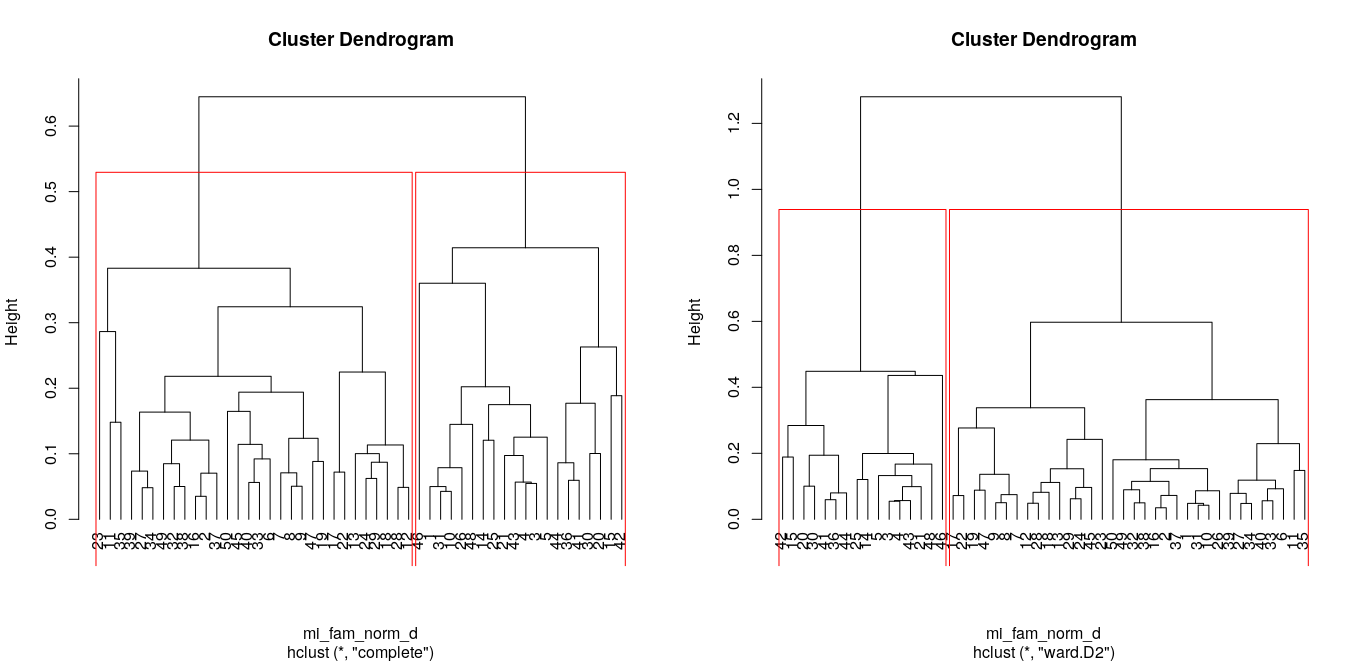
\includegraphics{grupos_ward_complete_altura_corte2.png}
\caption{Dendrogramas de los grupos producidos por Ward y Complete.
\label{fig:grupos_ward_complete_altura_corte2}}
\end{figure}

Se realizó un acercamiento restringido de la ordenación para probar el
grado de dependencia de los datos de la matriz de comunidad con la
matriz ambiental, mediante ajuste lineal en un análisis de redundancia
(RDA) (Borcard et al., 2018), utilizando la matriz de comunidad
transformada por Hellinger. Se seleccionaron las variables que
presentaron cierto grado de asociación, y (a discreción y de manera
secuencial) se excluyeron algunas de estas, con el objetivo de reducir
el grado de colinealidad entre las variables independientes restantes.

\subsection{Análisis de la
diversidad}\label{anuxe1lisis-de-la-diversidad}

Con la finalidad de asignar medidas apropiadas a la diversidad de
especies, y aprovechando su relación con los índices de Shannon y
Simpson, se empleó la serie de números de diversidad de Hill, la fórmula
de la entropía de Rengi y el índice de equidad de Pielou. Se examinó la
posible correlación entre estas medidas y las variables ambientales que
aparentaron tener algun efecto en la riqueza y equidad de la comunidad
(Borcard et al., 2018). Además, mediante interpolación por rarefacción
al número de individuos del cuadrante con la menor abundancia, se
compara el valor esperado de riqueza para todos los sitios.
Adicionalmente, se estima la riqueza de la familia Rubiaceae que
resultaría de aumentar al doble el muestreo realizado en BCI, mediante
los métodos de extrapolación incluidos en las colecciones de funciones
\texttt{SpadeR} y \texttt{iNEXT} (Chao, Ma, Hsieh, \& Chiu, 2016; Hsieh,
Ma, \& Chao, 2020), modificadas por Martínez Batlle (2020).

La variación en la composición y abundancia de especies de la comunidad,
es medida utilizando el índice multiplicativo de diversidad beta basado
en los números de Hill (Borcard et al., 2018). Finalmente, se examina la
contribución a la diversidad beta por parte de las especies y los sitios
en BCI, al analizar la varianza de la abundancia y riqueza de los
cuadrantes y las especies. Estos valores fueron comparados con la
varianza promedio, y se considera entonces que las especies cuya
varianza promedio supera la mitad de la varianza promedio total,
presentan una contribución importante a la diversidad beta de la
comunidad (Borcard et al., 2018).

\section{Resultados}\label{resultados}

La familia Rubiaceae en Barro Colorado se encuentra representada por 31
especies y 20 géneros. El género \emph{Psychotria} presenta la mayor
riqueza (8 especies). La tabla \ref{tab:abun_sp} resume las abundancias
de las especies de toda la comunidad, que en total suman 41,838
individuos, con una abundancia media de 65 individuos y mediana ubicada
en los 1,350 individuos. El gráfico de mosaicos de la figura
\ref{fig:abun_sp_q} presenta la riqueza numérica de las especies por
cuadrante. En el mismo se observa la marcada diferencia entre las
especies en cuanto a su incidencia. Además, el número de individuos de
las especies más abundantes, como \emph{Faramea occidentalis}, se
mantiene prácticamente constante en todos los cuadrantes. Por otro lado,
la abundancia de toda la comunidad muestra un aparente patrón en la
parte centro-occidental de BCI, donde se encuentran los sitios con la
mayor abundancia (ver figura \ref{fig:mapa_cuadros_abun_rubic}).

\begin{figure}
\centering
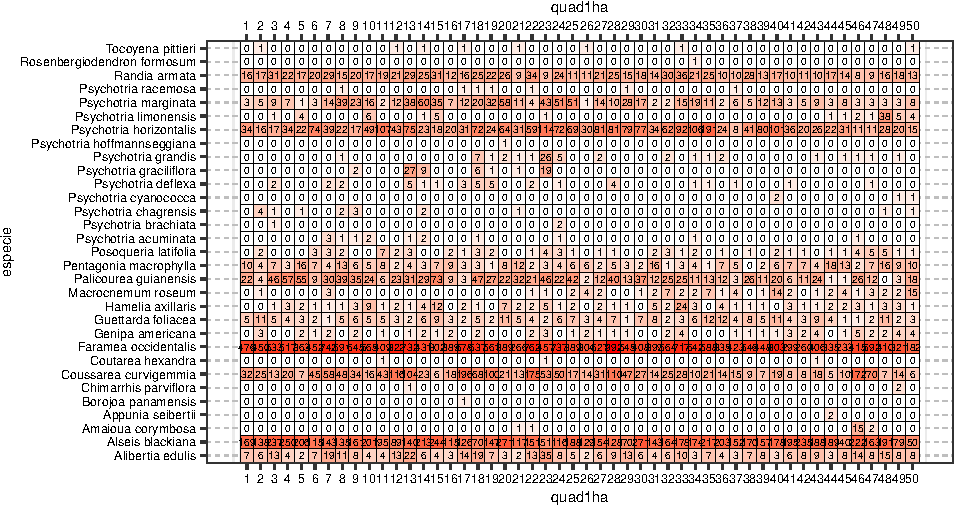
\includegraphics{manuscrito_files/figure-latex/unnamed-chunk-2-1.pdf}
\caption{\label{fig:abun_sp_q}Número de individuos de cada especie por
cuadrante.}
\end{figure}

\begin{figure}
\centering
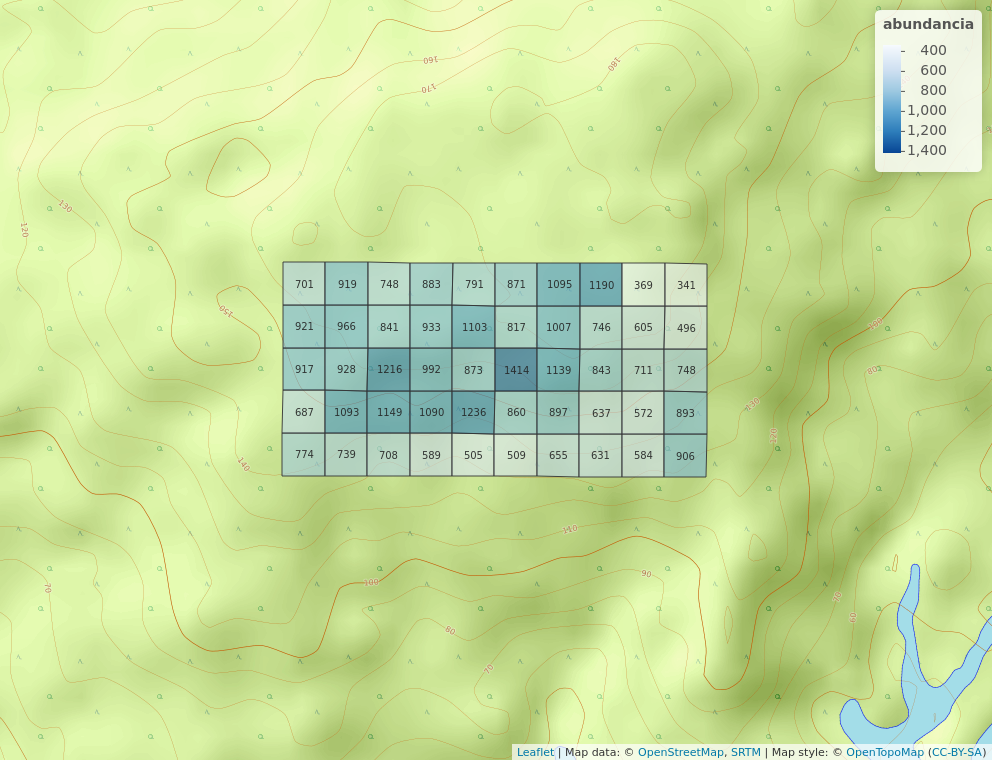
\includegraphics[width=0.75000\textwidth]{mapa_cuadros_abun_rubic.png}
\caption{Abundancia de rubiaceas en BCI
\label{fig:mapa_cuadros_abun_rubic}}
\end{figure}

Los valores para el coeficiente de Spearman presentados en el panel de
correlación de la figura \ref{fig:panel_cor_suelo_abun_riq_rubic_spear},
no mostraron evidencia de que exista relación entre la riqueza y la
abundancia especies con las variables geomorfológicas notadas en la
matriz de variables ambientales. Sin embargo, el mismo análisis sugiere
una posible relación entre la abundancia numérica de especies y la
compososición del suelo, mostrando relación positiva con valores altos
de aluminio y fósforo. Así como negativa, para valores altos de pH y
concentraciones de otros elementos.

\begin{figure}
\centering
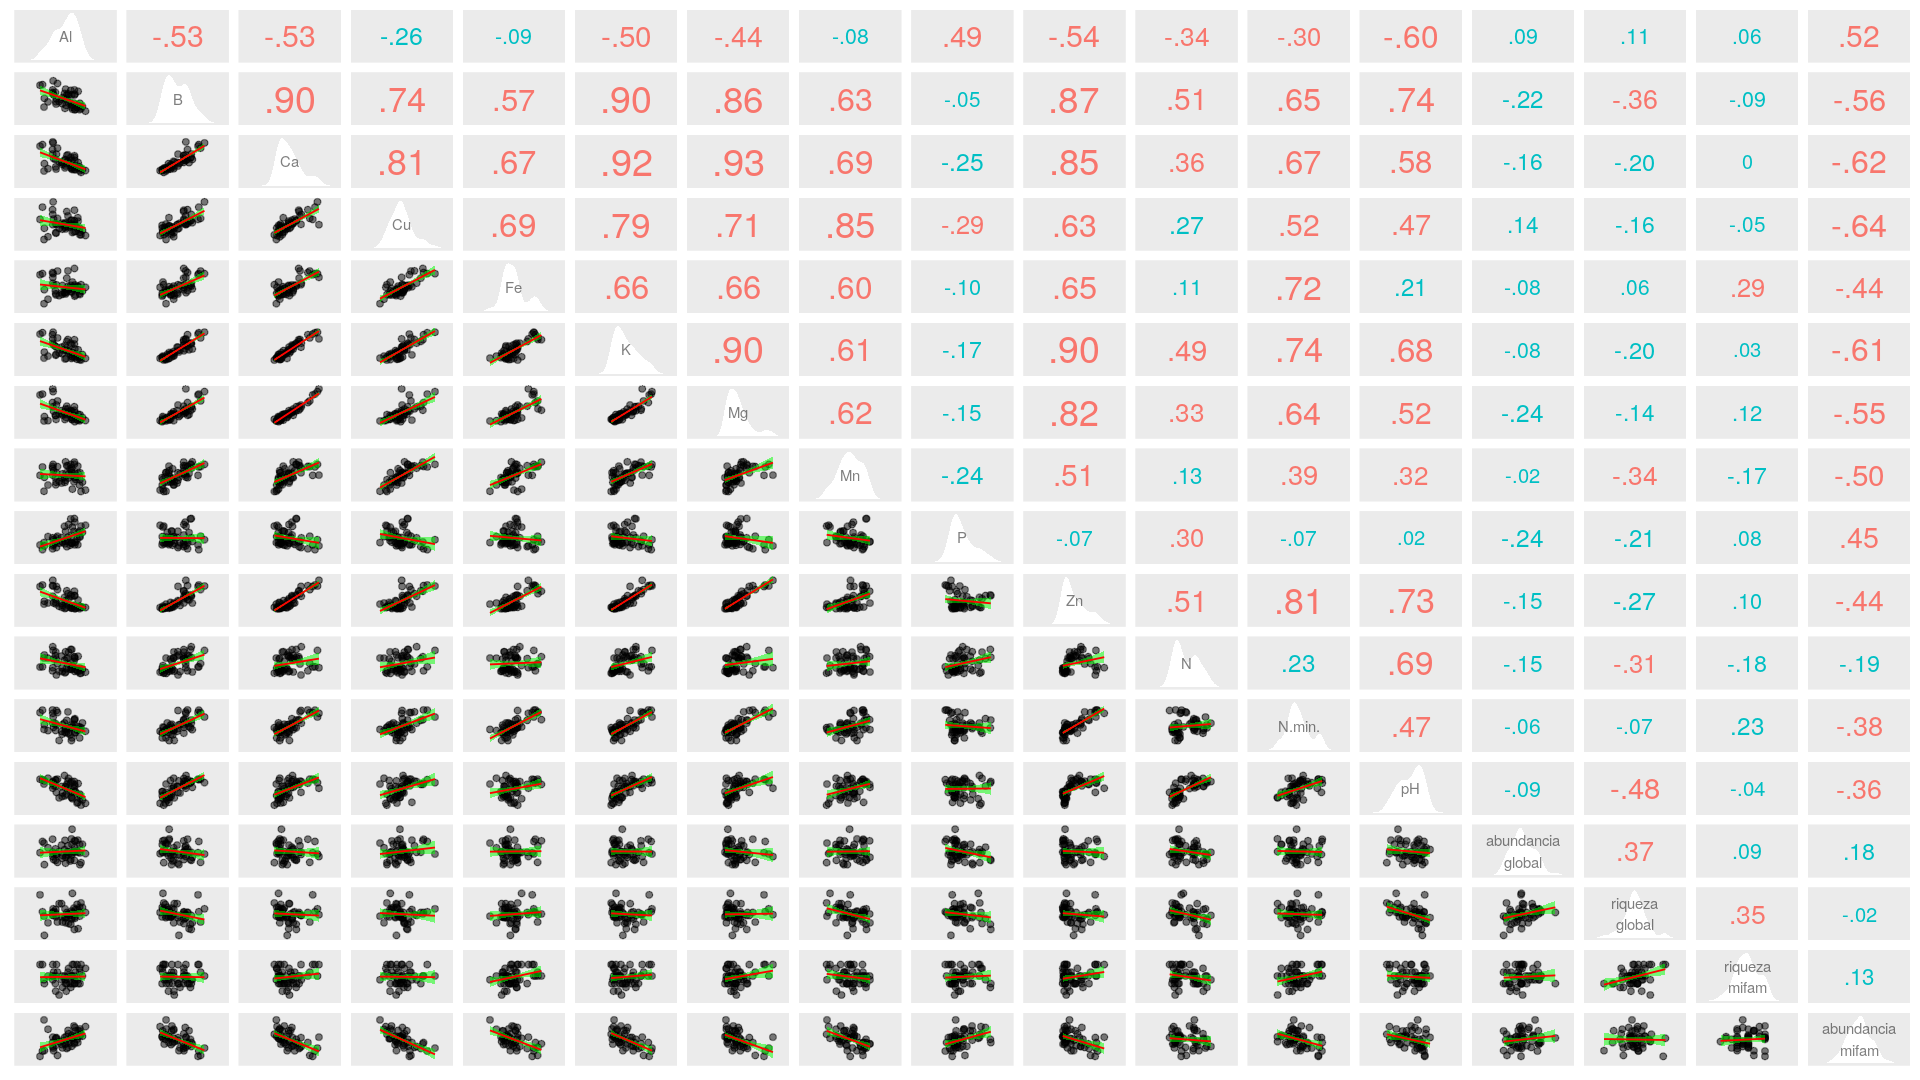
\includegraphics[width=0.80000\textwidth]{panel_cor_suelo_abun_riq_rubic_spear.png}
\caption{Panel de correlacion de Spearman entre los datos de la
comunidad y las variables edafológicas.
\label{fig:panel_cor_suelo_abun_riq_rubic_spear}}
\end{figure}

Las pruebas de correlación entre los grupos 1 y 2 formulados por
complete, resultaron significativas respecto a la variable fósforo. Por
otro lado, el contenido de cobre y la abundancia global promedio, es
decir, la media correspondiente a todas las plantas en BCI, son
significativamente diferentes entre los sitios de ambos grupos, para un
nivel de significancia de \(\alpha= 0.1\) (ver
\ref{fig:diagrama_caja_igualdad_medias_complete}).

El grupo 2 contiene los sitios con tendencia a presentar valores altos
de acidez y contenido de aluminio. Es probable que las especies
indicadoras del grupo con un mayor contenido de cobre estén mostrando
preferencia por estas condiciones ambientales. Indicios de esto, además,
pudieron observarse en los valores del índice de correlación de
Spearman, el cual indicaba una relación negativamente significa entre la
abundancia y el pH (ver mapas de las figuras \ref{fig:mapa_complete_k2}
y \ref{fig:mapa_cuadros_ph}). No obstante, el pH y la mayoría de
componentes del suelo en BCI tienen valores bastante homogéneos, y más
bien se presentan pequeños gradientes entre los cuadrantes, lo cual
evita que este tipo de acercamiento sea concluyente.

Las especies \emph{Alseis blackiana} y \emph{Psychotria limonensis}
fueron las que obtuvieron un valor alto de confianza al examinar su
potencial como especies indicadoras del grupo 1. Para el caso del grupo
2, las especies indicadoras fueron \emph{Faramea occidentalis},
\emph{Psychotria horizontalis} y \emph{Coussarea curvigemmia}. La
ocurrencia de \emph{A. blackiana} y \emph{Pentagonia macrophylla} indica
su preferencia por el grupo 1. Por otra parte, la muy dominante \emph{F.
occidentalis}, \emph{Psychotria deflexa}, \emph{P. racemosa}, \emph{P.
horizontalis}, \emph{Posoqueria latifolia}, \emph{Alibertia edulis} y
\emph{Coussarea curvigemmia} resultan de interes por ocurrir de manera
sistemática en el grupo 2.

\begin{figure}
\centering
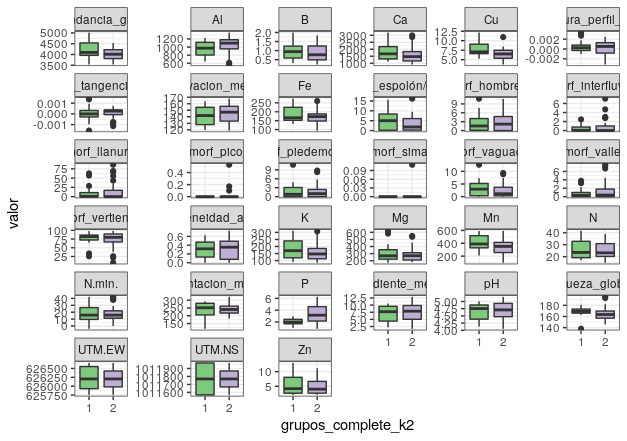
\includegraphics{diagrama_caja_igualdad_medias_complete.png}
\caption{Diagramas de caja de las variables que tuvieron un efecto,
según las pruebas de igualdad de medias. Los valores que presentan las
medianas de la variable fósforo son muy distintos entre el grupo 1
(verde) y el grupo 2 (gris).
\label{fig:diagrama_caja_igualdad_medias_complete}}
\end{figure}

\begin{figure}
\centering
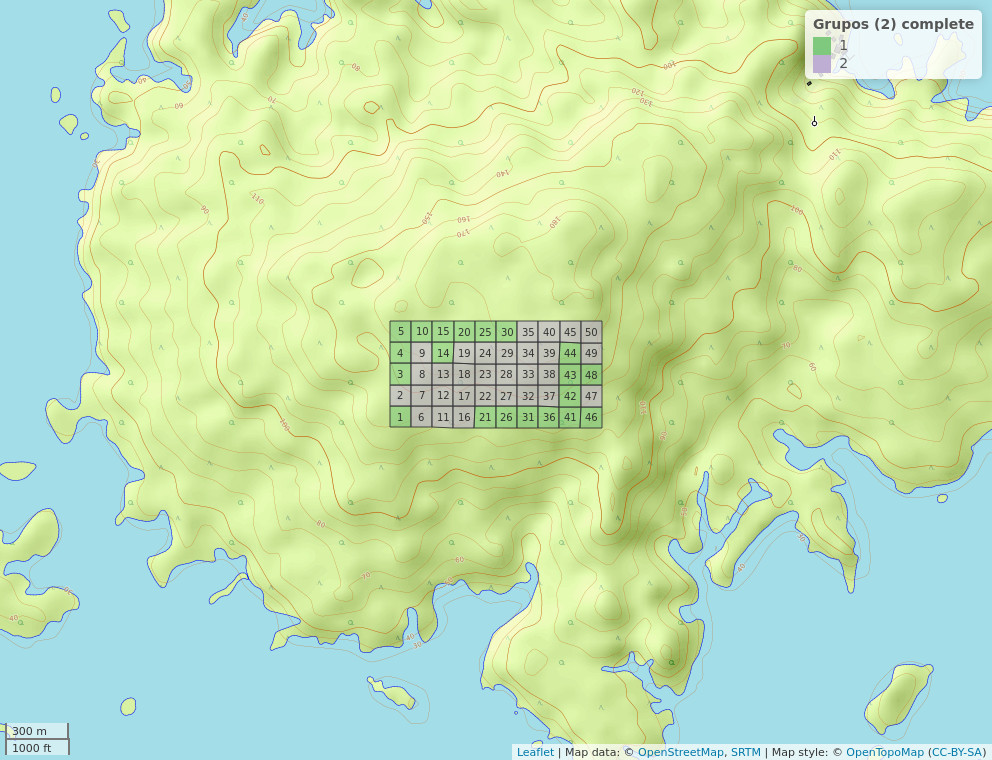
\includegraphics[width=0.75000\textwidth]{mapa_complete_k2.png}
\caption{Mapa en el que se presenta la repartición de sitios en los
grupos formulados por enlace completo. \label{fig:mapa_complete_k2}}
\end{figure}

\begin{figure}
\centering
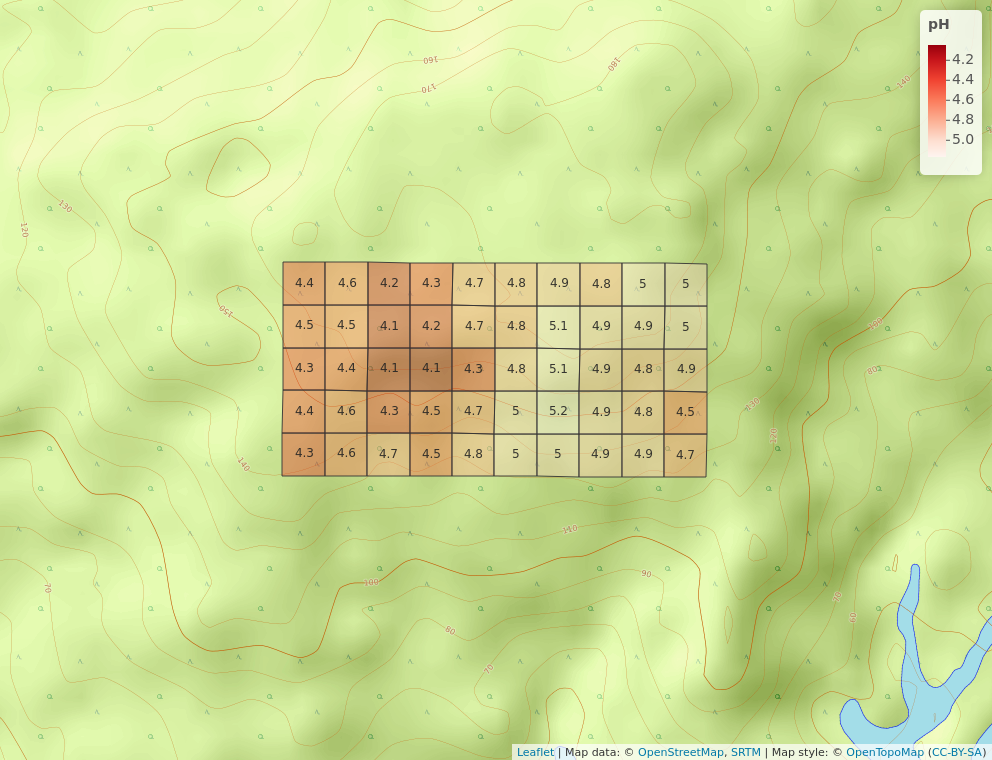
\includegraphics[width=0.75000\textwidth]{mapa_cuadros_ph.png}
\caption{pH del suelo en los cuadros de 1ha \label{fig:mapa_cuadros_ph}}
\end{figure}

En el diagrama rotulado como escalamiento 1 de la figura
\ref{fig:pca_biplot_suelo}, se observan tres grupos de cuadrantes
diferenciados entre sí. Un grupo de sitios con un alto grado de acidez y
contenido en aluminio, otro grupo caracterizado por la presencia de
elementos metálicos, y un tercero, con una cantidad de fósforo,
nitrógeno y valor de pH mayor. En el caso de las variables
geomorfológicas, algunos sitios están asociados a un alto porcentaje de
llanura y hombrera, aunque la mayoría se encuentra más cerca del origen
formado por los ejes de los componentes principales 1 y 2 (ver figura
\ref{fig:pca_biplot_geomorf}).

Los resultados del PCA de los datos de la matriz de comunidad se
encuentran resumidos en los diagramas de la figura
\ref{fig:pca_biplot_sps}. El escalamiento 1, muestra muchos de los
cuadrantes dispuestos alrededor del origen formado por los ejes, lo que
indica una contribución a la varianza relativamente equitativa por parte
de las especies. Sin embargo, aparecen también unos cuantos cuadrantes
con valores atípicos y más alejados. Se nota como las especies \emph{A.
blackiana}, \emph{C. curvigemmia}, \emph{P. marginalis} y \emph{P.
horizontalis}, presentan una contribución desproporcionada a la varianza
total, en comparación con el resto de las especies.

El escalamiento 2 de la figura
\ref{fig:biplot_correspndncia_sps_escal_2_2} en el análisis de
correspondencia mostró que las especies \emph{Psychotria graciliflora} y
\emph{Psychotria grandis} se encuentran asociadas. Ambas especies,
además, tienen valores de abundancia parecidos dentro de la comunidad
(65 y 57 individuos, respectivamente). Casi todas las demás especies se
encuentran próximas al punto de intersección, salvo aquellas que
presentaron una abundancia reducida, y en consecuencia, aparecen
cercanas a los pocos cuadrantes en los que se encuentran representadas.
La disparidad en la incidencia de las especies se refleja en su
disposición en el diagrama. Sin embargo, estos resultados no coinciden
del todo con los arrojados por el PCA de la matriz de distancias.

\begin{figure}
\centering
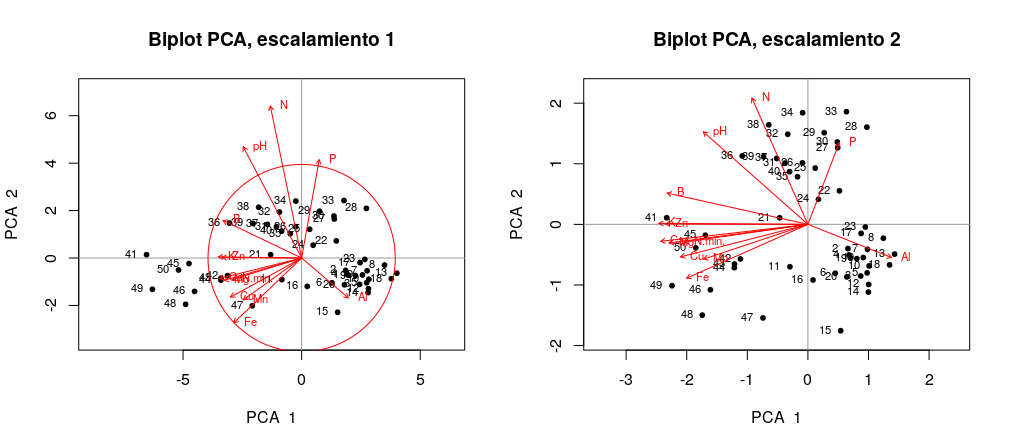
\includegraphics{pca_biplot_suelo.png}
\caption{Biplots generados en el PCA de las variables de suelo. Se
observa que las variables nitrógeno, fósforo y pH aportan la mayor parte
de la varianza explicada. La relación entre las variables se encuentra
debidamente representada en el recuadro del escalamiento 2, por medio de
los ángulos que forman sus vectores. \label{fig:pca_biplot_suelo}}
\end{figure}

\begin{figure}
\centering
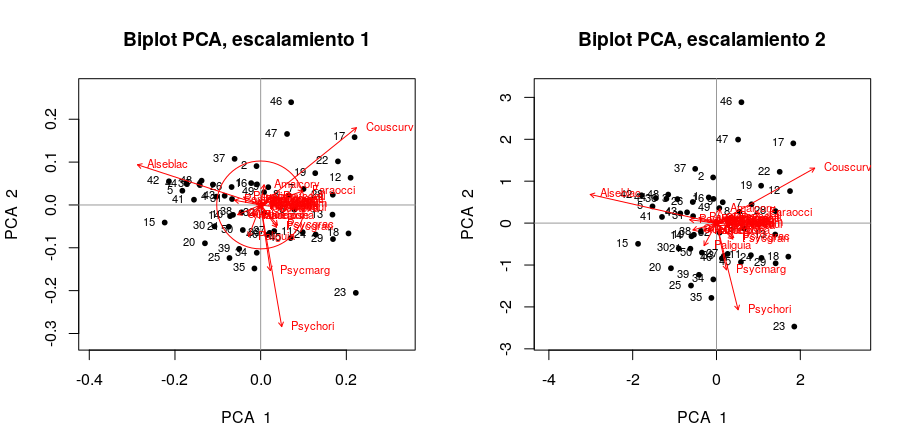
\includegraphics{pca_biplot_sps.png}
\caption{Biplots producidos por PCA de los datos de comunidad
transformados a distancias Hellinger. \label{fig:pca_biplot_sps}}
\end{figure}

\begin{figure}
\centering
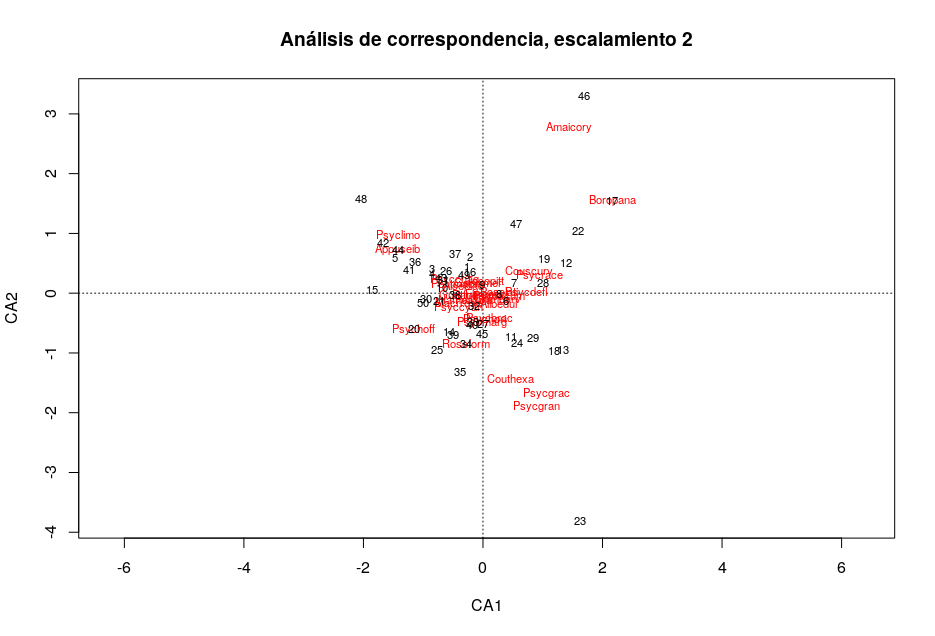
\includegraphics[height=0.65000\textwidth]{biplot_correspndncia_sps_escal_2_2.png}
\caption{Biplot del análisis de correspondencia de los datos de
abundancia de las especies de Rubiaceae.
\label{fig:biplot_correspndncia_sps_escal_2_2}}
\end{figure}

Se observa asociación entre el contenido de cobre, manganeso y fósforo
con algunos sitios y especies, en el \emph{biplot} del análisis de
coordenadas principales de la figura
\ref{fig:pcoa_sps_jacc_var_ambient}. También, algunas de las especies
menos abundantes de la comunidad se presentan asociadas a algunos sitios
comunes entre las mismas. Es probable que esta aparente asociación
aparezca debido a la combinación de una incidencia restringida por parte
de estas especies y al alto grado de autocorrelación entre los
cuadrantes.

Se destacan los patrones encontrados en los resultados de las pruebas de
asociación y los arrojados por el análisis de redundancia. En los
\emph{triplots} producidos por RDA (figura
\ref{fig:rda_triplot_var_selec_4_escal2}), se observó que
\emph{Psychotria horizontalis} y \emph{Psychotria marginata} se
encuentran asociadas a un grupo de cuadrantes, los que a su vez,
constituyen un microhabitat encontrado sobre una pequeña meseta en la
parte nor-oriental de BCI, y se diferencian además, por una elevada
concentración de fósforo y aluminio en el suelo. Por otro lado, la
especie \emph{Alseis blackiana} presenta asociación con el contenido de
metales como manganeso, hierro y cobre. Esto último coincide con los
resultados vistos en el PCA, lo que demuestra cierto grado de
preferencia hacia estas condiciones ambientales por parte de esta
especie.

\begin{figure}
\centering
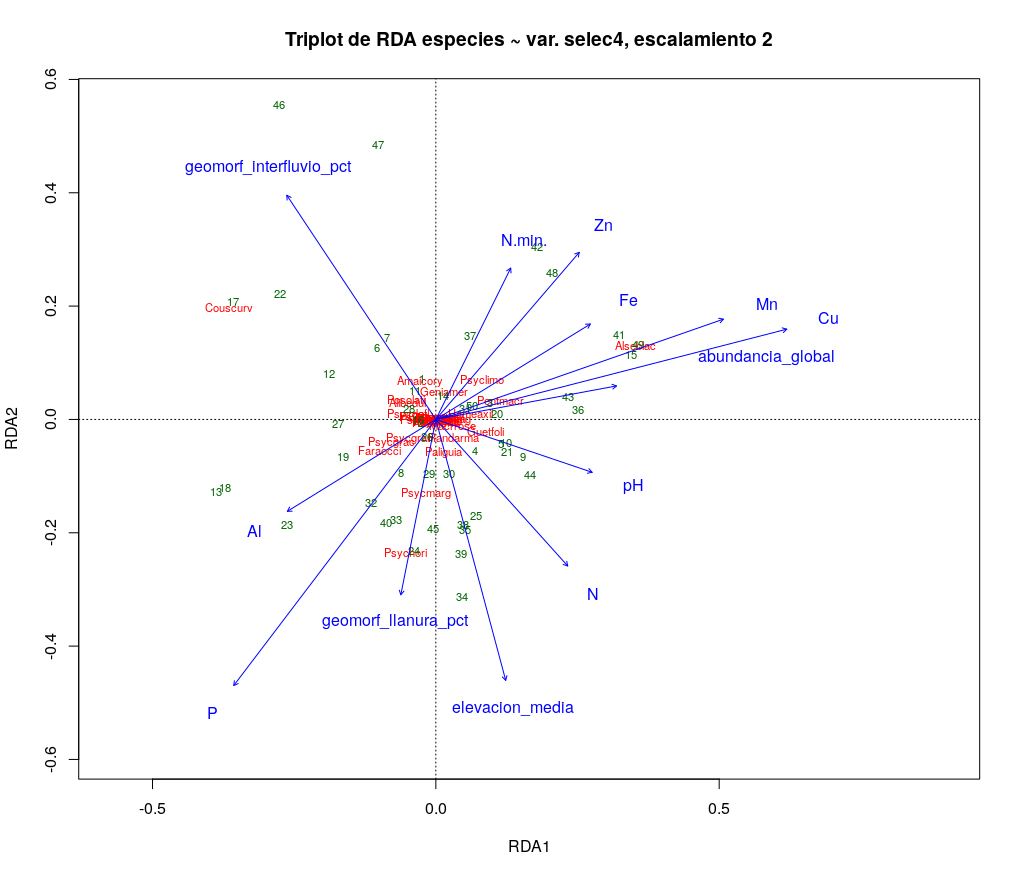
\includegraphics[height=0.70000\textwidth]{rda_triplot_var_selec_4_escal2.png}
\caption{Triplot del RDA de los valores de abundancia transformados. Las
variables ambientales que se observan son aquellas que fueron
seleccionadas para restringir la varianza explicada de los datos de
comunidad. \label{fig:rda_triplot_var_selec_4_escal2}}
\end{figure}

La riqueza de la familia Rubiaceae aumenta en función del contenido de
hierro, nitrógeno y nitrógeno mineralizado. La equidad pareciera tambien
estar asociada con estas variables, además de que la misma es mayor
hacia el norte de BCI
(\ref{fig:panel_cor_indics_diversidad1_columnnas_quitadas}).

Aparte del cuadrante \#50, los sitios con la mayor riqueza presentan
también mucha abundancia. El cuadrante \#1, con la menor riqueza,
presenta una de las mayores dominancias. Sucede algo similar en el
cuadrante \#28, aunque en este caso el valor riqueza de especies
presentado no es tan bajo, sino que en comparación, contiene una
desorbitada abundancia (1414 individuos).

Las especies que contribuyen de manera significativa a la diversidad
beta, fueron las que también resultaron ser indicadoras debido a su
incidencia en los grupos 1 y 2. Con la excepción de la especie
\emph{Macrocnemum roseum}, la cual tiene una abundancia mucho menor que
la de las demás especies que resultan de este análisis.

La riqueza de especies (número de Hill 0 en el gráfico de la figura
\ref{fig:grafico_divrsdad_beta_hill}) presenta la mayor contribución a
la medida de diversidad beta para la comunidad. Así sucede, ya que la
abundancia de las especies dominantes no varía drásticamente entre
cuadrantes, y es precisamente su composición de especies lo que
diferencia a los sitios entre sí.

\begin{figure}
\centering
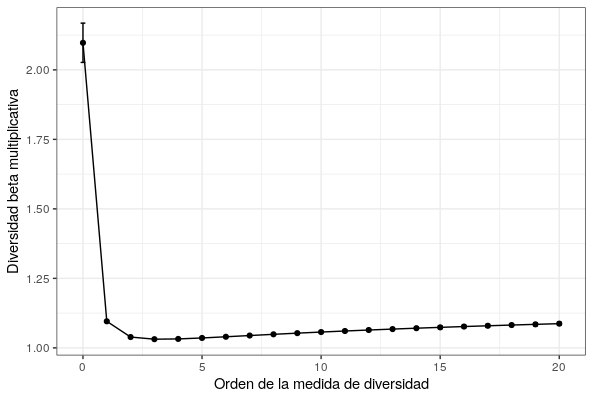
\includegraphics[height=0.50000\textwidth]{grafico_divrsdad_beta_hill.png}
\caption{Gráfico de la diversidad beta multiplicativa en función de los
números de diversidad en la serie de Hill.
\label{fig:grafico_divrsdad_beta_hill}}
\end{figure}

\begin{figure}
\centering
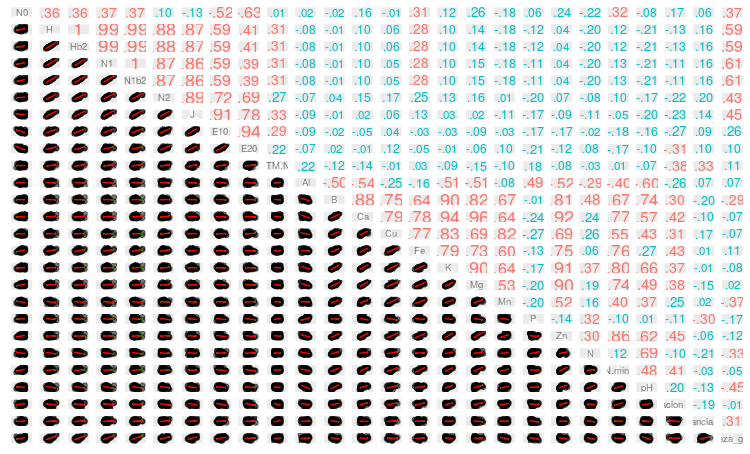
\includegraphics[height=0.50000\textwidth]{panel_cor_indcs_diversidad1_columnas_quitadas.png}
\caption{Correlación entre diversidad/equidad y algunas de las variables
ambientales destacadas. \(N0\): riqueza de especies; \(H\): entropía de
Shannon; \(Hb2\): entropía de Shannon con 2 como base del logaritmo;
\(N1\) y \(N2\): Números de Hill; \(N1b2\): Número de Hill 1 en base log
2; \(J\): Equidad de Pielou; \(E10\) y \(E20\): ratios de Hill 1 y 2.
\label{fig:panel_cor_indics_diversidad1_columnnas_quitadas}}
\end{figure}

\section{Discusión}\label{discusiuxf3n}

Se confirma que variables ambientales como el contenido de alumínio y
fósforo en el suelo, tienen un efecto al caracterizar la abundancia
relativa de las especies de la familia Rubiaceae. Adicionalmente, esta
comunidad podría dividirse en dos grupos más o menos diferenciados entre
sí por su preferencia, o más bien tolerancia, al contenido de cobre en
el suelo. Otros autores se han referido con anterioridad a la tolerancia
a los metales pesados que presentan algunas de las especies de esta
familia (McAlister, Kolterman, \& Pollard, 2015). Lo que hace remarcable
el hecho de que pruebas de este fenómeno puedan apreciarse a un nivel
muy local.

Algunas de las pruebas estadísticas empleadas en este estudio requieren
del supuesto de independencia entre muestras, supuesto que es incumplido
por los cuadrantes en BCI debido a su contigüidad. Sin embargo, esta
condición permitió un acercamiento comparativo con las técnicas
apropiadas para el análisis de muestras con cierto grado asociación
entre sí. Además, en BCI, tanto las variables ambientales como las
comunidades de plantas se encuentran correlacionadas espacialmente. El
área correspondiente a la parcela es bastante homogénea en cuanto a sus
condiciones físicas, ya que fué diseñada para que así fuera (Baillie,
Elsenbeer, Barthold, Grimm, \& Stallard, 2006). Como la misma se
encuentra situada sobre el dorso de una cuesta de andesita, las
variables edafológicas aquí presentes en su mayoría siguen un gradiente
a lo largo de todo BCI, resultado de la meteorización de la roca
original (Patino, Velbel, Price, \& Wade, 2003). Por lo tanto, es
razonable considerar que los patrones encontrados entre métodos
contrastados son evidencia del grado de importancia que presentan las
condiciones ambientales (especialmente las relacionadas con la
composición química del suelo) en la estructuración de esta comunidad de
especies en BCI.

Las especies con preferencia por el grupo 1 evaden sistemáticamente al
grupo 2 y viceversa. Esta diferenciación en la ocurrencia de las
especies menos comunes no se explica del todo con las variables
ambientales medidas en BCI y es posible que exista algun otro factor que
determina la ordenación de esta comunidad de plantas. La cobertura del
dosel arbóreo podría ser una de estas variables a considerarse, puesto
que las especies dominantes en la comunidad son a la vez tolerantes a la
sombra (Grandtner \& Chevrette, 2013).

Los resultados expuestos en este trabajo muestran como el estudio de la
estructura de las comunidades ecológicas puede presentar complicasiones
cuando nos enfrentamos a taxónes muy diversos, para los cuales las
medidas de abundancia relativa convencionales podrían ver su eficacia
limitada (Ricotta, 2004). Además, los análisis de agrupamiento aquí
realizados pudieron haberse visto sesgados por la heterogeneidad
morfométrica que presentan las especies de Rubiaceae. Estas plantas
pueden tener diversos hábitos de crecimiento, desde porte herbáceo y
arbustivo a árboles relativamente grandes. Esto hace que el hecho de que
se incluya el criterio de dap de 10 mm en el momento de ser censadas
podría estar excluyendo especies clave en el rompecabezas.

\section*{Información de soporte} \label{inf_supletary}

\beginsupplement

\begin{longtable}[]{@{}lr@{}}
\caption{\label{tab:abun_sp}Abundancia total por
especie.}\tabularnewline
\toprule
Latin & n\tabularnewline
\midrule
\endfirsthead
\toprule
Latin & n\tabularnewline
\midrule
\endhead
Faramea occidentalis & 24989\tabularnewline
Alseis blackiana & 7928\tabularnewline
Psychotria horizontalis & 2453\tabularnewline
Coussarea curvigemmia & 2010\tabularnewline
Palicourea guianensis & 1118\tabularnewline
Randia armata & 937\tabularnewline
Psychotria marginata & 761\tabularnewline
Alibertia edulis & 417\tabularnewline
Pentagonia macrophylla & 306\tabularnewline
Guettarda foliacea & 252\tabularnewline
Hamelia axillaris & 128\tabularnewline
Macrocnemum roseum & 87\tabularnewline
Posoqueria latifolia & 73\tabularnewline
Psychotria limonensis & 70\tabularnewline
Genipa americana & 67\tabularnewline
Psychotria graciliflora & 65\tabularnewline
Psychotria grandis & 57\tabularnewline
Psychotria deflexa & 38\tabularnewline
Amaioua corymbosa & 19\tabularnewline
Psychotria chagrensis & 16\tabularnewline
Psychotria acuminata & 14\tabularnewline
Tocoyena pittieri & 8\tabularnewline
Psychotria racemosa & 7\tabularnewline
Psychotria cyanococca & 4\tabularnewline
Chimarrhis parviflora & 3\tabularnewline
Coutarea hexandra & 3\tabularnewline
Psychotria brachiata & 3\tabularnewline
Appunia seibertii & 2\tabularnewline
Borojoa panamensis & 1\tabularnewline
Psychotria hoffmannseggiana & 1\tabularnewline
Rosenbergiodendron formosum & 1\tabularnewline
\bottomrule
\end{longtable}

\begin{figure}
\centering
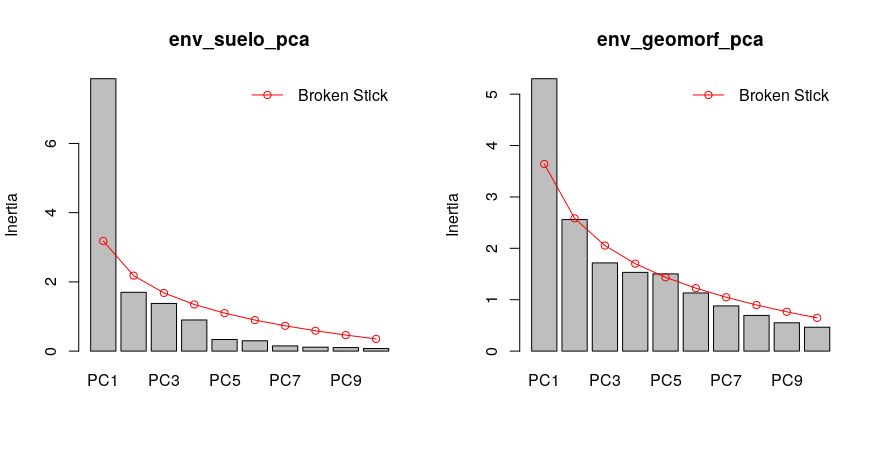
\includegraphics{env_suelo_geomorf_pca_br_stick.png}
\caption{Componentes príncipales de la varianza en las variables de
suelo y geomorfología en BCI. En estos gráficos se incluye el
comportamiento de la varianza explicada, predecido por el modelo de bara
quebrada, representado por la línea roja formando la curva. (La escala
denominada ``\emph{Inertia}'' representa la suma de los cuadrados de
toda la varianza). \label{fig:pca_suelo_geomorf_br_stick}}
\end{figure}

\begin{figure}
\centering
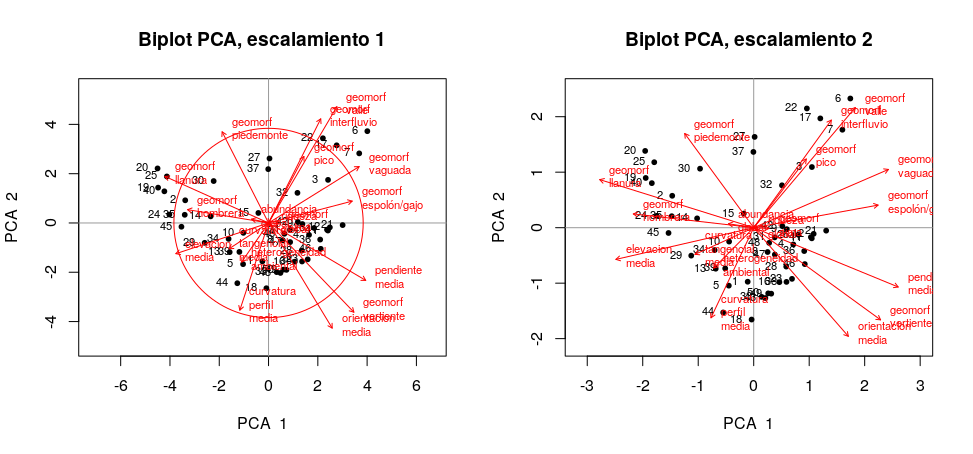
\includegraphics{pca_biplot_geomorf.png}
\caption{Biplots generados por PCA de las variables geomorfológicas.
\label{fig:pca_biplot_geomorf}}
\end{figure}

\begin{figure}
\centering
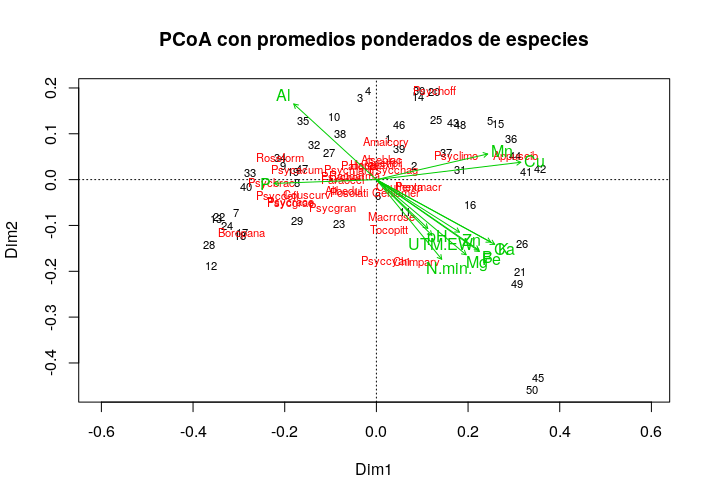
\includegraphics{pcoa_sps_jacc_var_ambient.png}
\caption{Biplot de PCoA de las distancias de Jaccard. Las distancias
entre especies están ponderadas en base a sus valores de abundancia.
\label{fig:pcoa_sps_jacc_var_ambient}}
\end{figure}

\begin{figure}
\centering
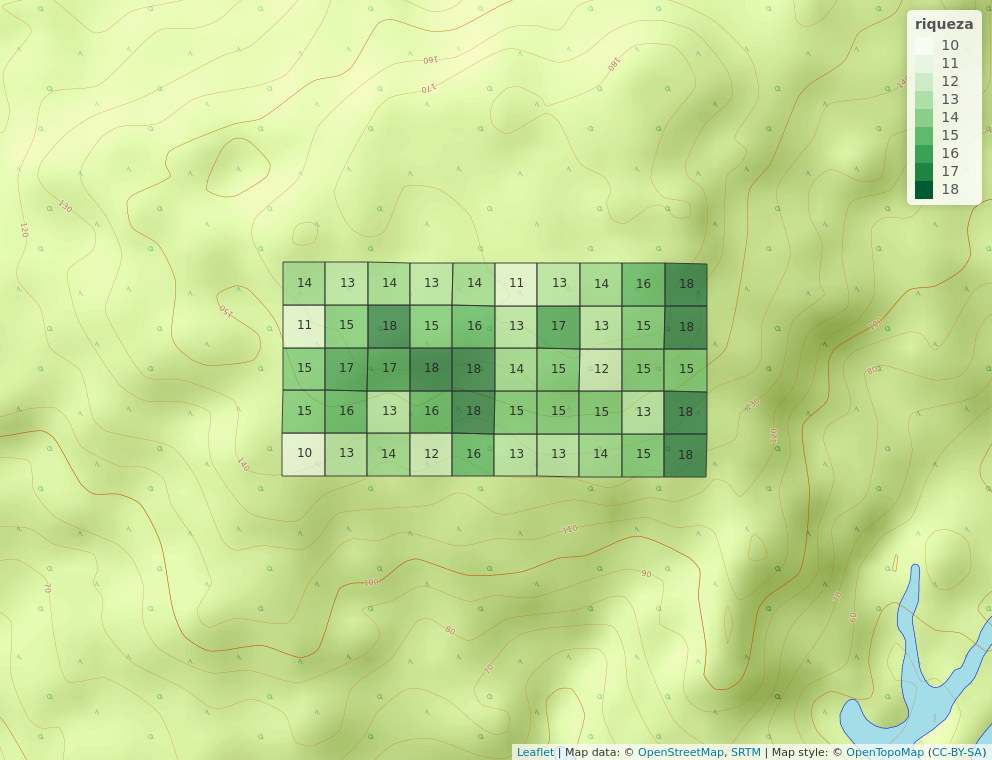
\includegraphics{mapa_cuadros_riq_rubic.png}
\caption{Distribución de la riqueza de rubiaceas en BCI
\label{fig:mapa_cuadros_riq}}
\end{figure}

\begin{figure}
\centering
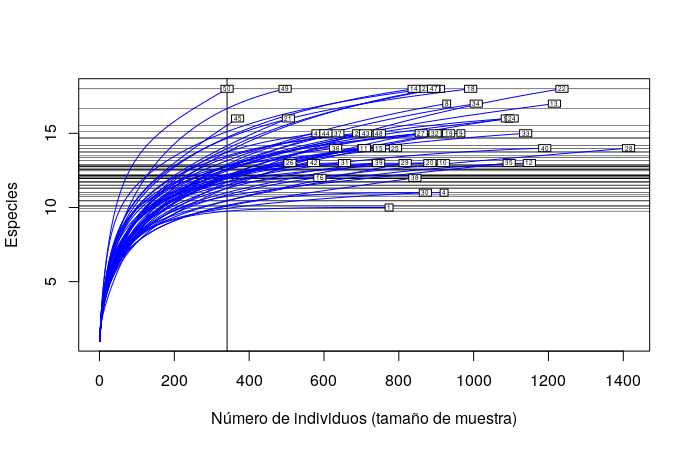
\includegraphics{rarefaccion_min_abun.png}
\caption{Curva de rarefacción. Las barras horizontales muestran el valor
de la riqueza esperada en cada sitio al interpolar las muestras hacia la
abundancia mínima observada (341 individuos), presentada por el
cuadrante \#50. \label{fig:rarefaccion_min_abun}}
\end{figure}

\begin{figure}
\centering
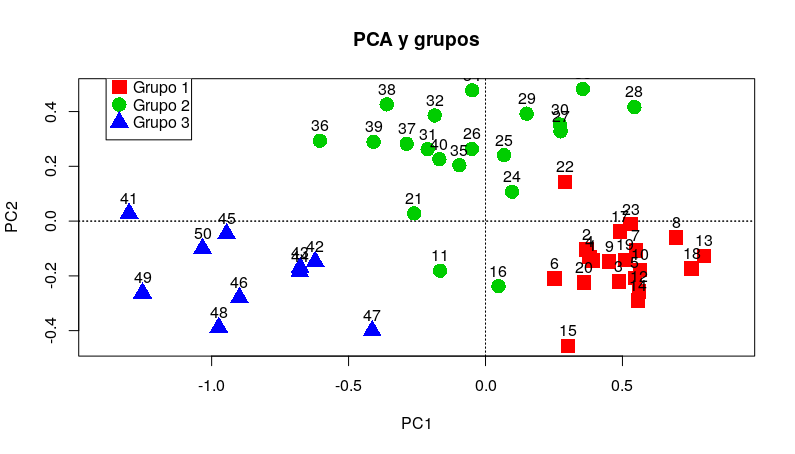
\includegraphics{grafico_pca_suelo.png}
\caption{Diagrama PCA de los grupos de cuadrantes según variables de
suelo \label{fig:grafico_pca_suelo}}
\end{figure}

\begin{figure}
\centering
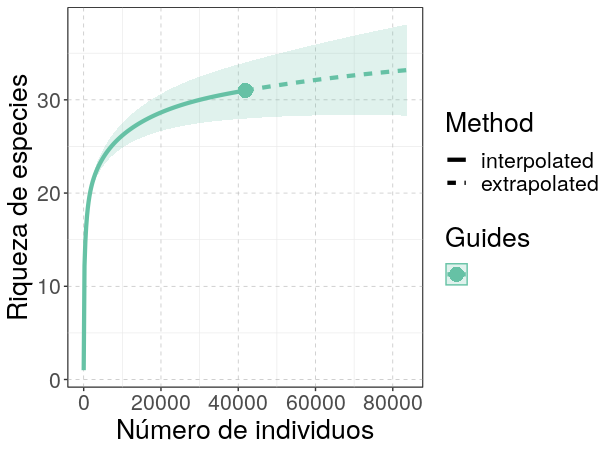
\includegraphics[height=0.45000\textwidth]{curva_extrapol_doble_esfuerzo.png}
\caption{Curva de acumulación de especies hacia el doble de la
abundancia encontrada en BCI. Se estima que la riqueza aumentaría en
cuatro especies en consecuencia de duplicar el senso, o replicarlo en
otra zona de Barro Colorado. El intervalo para un 95\% de confianza se
representa con los márgenes verde pálido.
\label{fig:curva_extrapol_doble_esfuerzo}}
\end{figure}

\section*{\texorpdfstring{\emph{Script}
reproducible}{Script reproducible}}\label{script-reproducible}
\addcontentsline{toc}{section}{\emph{Script} reproducible}

\subsection*{aed\_Rub.R}\label{aed_rub.r}
\addcontentsline{toc}{subsection}{aed\_Rub.R}

\begin{Shaded}
\begin{Highlighting}[]
\CommentTok{#' ---}
\CommentTok{#' title: "Análisis exploratorio de datos. Riqueza y abundancia"}
\CommentTok{#' author: "JR"}
\CommentTok{#' date: "13 de octubre, 2020"}
\CommentTok{#' output: github_document}
\CommentTok{#' ---}

\CommentTok{#' }\AlertTok{###}\CommentTok{ Área de cargar paquetes}
\KeywordTok{library}\NormalTok{(vegan)}
\KeywordTok{library}\NormalTok{(tidyverse)}
\KeywordTok{library}\NormalTok{(sf)}
\KeywordTok{source}\NormalTok{(}\StringTok{'biodata/funciones.R'}\NormalTok{)}

\CommentTok{#' }\AlertTok{###}\CommentTok{ Área de cargar datos}
\CommentTok{#' Censo (el objeto se carga con prefijo "censo") y matriz de comunidad (prefijo "mc")}
\KeywordTok{load}\NormalTok{(}\StringTok{'biodata/Rubiaceae.Rdata'}\NormalTok{)}
\KeywordTok{load}\NormalTok{(}\StringTok{'biodata/matriz_ambiental.Rdata'}\NormalTok{) }\CommentTok{#Matriz ambiental, se carga como "bci_env_grid"}

\CommentTok{#' }\AlertTok{###}\CommentTok{ Imprimir datos en pantalla (impresiones parciales con head)}
\KeywordTok{head}\NormalTok{(censo_rubic)}
\KeywordTok{head}\NormalTok{(mc_rubic)}
\NormalTok{bci_env_grid }\CommentTok{# No necesita imprimirse parcialmente}

\CommentTok{#' }\AlertTok{###}\CommentTok{ También podemos usar}
\CommentTok{#' Requiere que se haya cargado ya la colección tidyverse}
\NormalTok{censo_rubic }\OperatorTok\StringTok{ }\NormalTok{tibble}
\NormalTok{mc_rubic }\OperatorTok\StringTok{ }\NormalTok{tibble}

\CommentTok{#' }\AlertTok{###}\CommentTok{ Lista de especies}
\KeywordTok{sort}\NormalTok{(}\KeywordTok{colnames}\NormalTok{(mc_rubic))}

\CommentTok{#' }\AlertTok{###}\CommentTok{ Número de sitios, tanto en matriz de comunidad como en ambiental}
\CommentTok{#' Verifica que coinciden}
\KeywordTok{nrow}\NormalTok{(mc_rubic) }\CommentTok{#En la matriz de comunidad}
\KeywordTok{nrow}\NormalTok{(bci_env_grid) }\CommentTok{#En la matriz ambiental}

\CommentTok{#' }\AlertTok{###}\CommentTok{ Riqueza numérica de especies (usando matriz de comunidad) por quadrat}
\CommentTok{#' Nota: cargar paquete vegan arriba, en el área de paquetes}
\KeywordTok{specnumber}\NormalTok{(mc_rubic)}
\KeywordTok{sort}\NormalTok{(}\KeywordTok{specnumber}\NormalTok{(mc_rubic)) }\CommentTok{# Ordenados ascendentemente}
\KeywordTok{summary}\NormalTok{(}\KeywordTok{specnumber}\NormalTok{(mc_rubic)) }\CommentTok{# Resumen estadístico}

\CommentTok{#' }\AlertTok{###}\CommentTok{ Abundancia de especies por quadrat}
\KeywordTok{sort}\NormalTok{(}\KeywordTok{rowSums}\NormalTok{(mc_rubic))}
\KeywordTok{summary}\NormalTok{(}\KeywordTok{rowSums}\NormalTok{(mc_rubic)) }\CommentTok{# Resumen estadístico}

\CommentTok{#' }\AlertTok{###}\CommentTok{ Abundancia por especie}
\KeywordTok{sort}\NormalTok{(}\KeywordTok{colSums}\NormalTok{(mc_rubic))}
\KeywordTok{summary}\NormalTok{(}\KeywordTok{colSums}\NormalTok{(mc_rubic)) }\CommentTok{# Resumen estadístico}

\CommentTok{#' }\AlertTok{###}\CommentTok{ Riqueza numérica de toda la "comunidad"}
\KeywordTok{specnumber}\NormalTok{(}\KeywordTok{colSums}\NormalTok{(mc_rubic))}

\CommentTok{#' }\AlertTok{###}\CommentTok{ Abundancia de toda la comunidad}
\KeywordTok{sum}\NormalTok{(}\KeywordTok{colSums}\NormalTok{(mc_rubic))}

\CommentTok{#' }\AlertTok{###}\CommentTok{ Una tabla para el manuscrito, es necesario asignarle nombre}
\CommentTok{#' Para esto, usaré la colección "tidyverse"}
\NormalTok{abun_sp <-}\StringTok{ }\NormalTok{censo_rubic }\OperatorTok
\StringTok{  }\KeywordTok{group_by}\NormalTok{(Latin) }\OperatorTok\StringTok{ }
\StringTok{  }\KeywordTok{count}\NormalTok{() }\OperatorTok\StringTok{ }
\StringTok{  }\KeywordTok{arrange}\NormalTok{(}\KeywordTok{desc}\NormalTok{(n))}
\NormalTok{abun_sp}

\CommentTok{#' }\AlertTok{###}\CommentTok{ Un gráfico para el manuscrito}
\CommentTok{#' Gráfico de mosaicos de la abundancia por especie por cuadros}
\NormalTok{abun_sp_q <-}\StringTok{ }\KeywordTok{crear_grafico_mosaico_de_mc}\NormalTok{(mc_rubic, }\DataTypeTok{tam_rotulo =} \DecValTok{7}\NormalTok{)}
\NormalTok{abun_sp_q}
\end{Highlighting}
\end{Shaded}

\subsection*{aed5\_correlacion\_variables\_ambientales.R}\label{aed5_correlacion_variables_ambientales.r}
\addcontentsline{toc}{subsection}{aed5\_correlacion\_variables\_ambientales.R}

\begin{Shaded}
\begin{Highlighting}[]
\CommentTok{#' ---}
\CommentTok{#' title: "Análisis exploratorio de datos. Correlaciones entre variables ambientales"}
\CommentTok{#' author: "JR"}
\CommentTok{#' date: "25 de octubre, 2020"}
\CommentTok{#' output: github_document}
\CommentTok{#' ---}

\NormalTok{knitr}\OperatorTok{::}\NormalTok{opts_chunk}\OperatorTok{$}\KeywordTok{set}\NormalTok{(}\DataTypeTok{fig.width=}\DecValTok{12}\NormalTok{, }\DataTypeTok{fig.height=}\DecValTok{8}\NormalTok{)}

\CommentTok{#' }\AlertTok{###}\CommentTok{ Cargar paquetes}
\KeywordTok{library}\NormalTok{(tidyverse)}
\KeywordTok{library}\NormalTok{(sf)}
\KeywordTok{library}\NormalTok{(ez)}
\KeywordTok{library}\NormalTok{(psych)}
\KeywordTok{library}\NormalTok{(vegan)}
\KeywordTok{library}\NormalTok{(graphics)}

\CommentTok{#' }\AlertTok{###}\CommentTok{ Cargar datos}
\KeywordTok{load}\NormalTok{(}\StringTok{'biodata/matriz_ambiental.Rdata'}\NormalTok{)}
\KeywordTok{load}\NormalTok{(}\StringTok{'biodata/Rubiaceae.Rdata'}\NormalTok{)}

\CommentTok{#' }\AlertTok{###}\CommentTok{ Una correlación simple}
\KeywordTok{cor}\NormalTok{(bci_env_grid}\OperatorTok{$}\NormalTok{pendiente_media, bci_env_grid}\OperatorTok{$}\NormalTok{geomorf_vertiente_pct)}
\KeywordTok{plot}\NormalTok{(bci_env_grid}\OperatorTok{$}\NormalTok{pendiente_media, bci_env_grid}\OperatorTok{$}\NormalTok{geomorf_vertiente_pct)}
\KeywordTok{cor.test}\NormalTok{(bci_env_grid}\OperatorTok{$}\NormalTok{pendiente_media, bci_env_grid}\OperatorTok{$}\NormalTok{geomorf_vertiente_pct)}

\CommentTok{#' }\AlertTok{###}\CommentTok{ Generar objeto de columnas numéricas}
\CommentTok{#' El objeto que generaré, denominado `env_num`, no tendrá las columnas `id` y las de coordenadas UTM, y añadiré la abundancia y riqueza de mi familia. Al mismo tiempo, insertaré un enter (`\textbackslash{}n`) en nombres largos de variables, para acomodar los nombres de variables al panel de correlaciones; por ejemplo, el nombre `riqueza_global` se renombra a `riqueza\textbackslash{}nglobal`.}
\NormalTok{env_num <-}\StringTok{ }\NormalTok{bci_env_grid }\OperatorTok
\StringTok{  }\NormalTok{dplyr}\OperatorTok{::}\KeywordTok{select_if}\NormalTok{(is.numeric) }\OperatorTok
\StringTok{  }\NormalTok{dplyr}\OperatorTok{::}\KeywordTok{select}\NormalTok{(}\OperatorTok{-}\NormalTok{id, }\OperatorTok{-}\KeywordTok{matches}\NormalTok{(}\StringTok{'^U.*'}\NormalTok{)) }\OperatorTok\StringTok{ }
\StringTok{  }\NormalTok{st_drop_geometry }\OperatorTok\StringTok{ }
\StringTok{  }\KeywordTok{mutate}\NormalTok{(}
    \DataTypeTok{riqueza_mifam =} \KeywordTok{specnumber}\NormalTok{(mc_rubic),}
    \DataTypeTok{abundancia_mifam =} \KeywordTok{rowSums}\NormalTok{(mc_rubic)) }\OperatorTok\StringTok{ }
\StringTok{  }\KeywordTok{rename_all}\NormalTok{(gsub, }\DataTypeTok{pattern =} \StringTok{'_pct$'}\NormalTok{, }\DataTypeTok{replacement =} \StringTok{''}\NormalTok{) }\OperatorTok\StringTok{ }
\StringTok{  }\KeywordTok{rename_all}\NormalTok{(gsub, }\DataTypeTok{pattern =} \StringTok{'_| '}\NormalTok{, }\DataTypeTok{replacement =} \StringTok{'}\CharTok{\textbackslash{}n}\StringTok{'}\NormalTok{)}
\NormalTok{env_num }\OperatorTok\StringTok{ }\NormalTok{tibble}

\CommentTok{#' }\AlertTok{###}\CommentTok{ Panel de correlaciones con herramientas del paquete `graphics` y `psych`}
\KeywordTok{cor}\NormalTok{(env_num)}
\KeywordTok{ncol}\NormalTok{(env_num)}
\KeywordTok{pairs}\NormalTok{(env_num[,}\KeywordTok{sample}\NormalTok{(}\DecValTok{1}\OperatorTok{:}\DecValTok{33}\NormalTok{, }\DecValTok{15}\NormalTok{)]) }\CommentTok{# paquete graphics}
\NormalTok{env_num[,}\KeywordTok{sample}\NormalTok{(}\DecValTok{1}\OperatorTok{:}\DecValTok{33}\NormalTok{, }\DecValTok{15}\NormalTok{)] }\OperatorTok\StringTok{ }\NormalTok{pairs.panels }\CommentTok{#paquete psych}

\CommentTok{#' }\AlertTok{###}\CommentTok{ Panel de correlaciones con `ez`}
\CommentTok{#' }
\CommentTok{#' #### Todas las variables (se empasta). Comentado, sólo mostrado para fines didácticos}
\CommentTok{# p_cor_todos <- env_num %>%}
\CommentTok{#   ezCor(r_size_lims = c(4,8), label_size = 4)}
\CommentTok{# p_cor_todos}

\CommentTok{#' #### Sólo suelo (elementos y pH), abundancia/riqueza}
\NormalTok{p_cor_suelo_ar <-}\StringTok{ }\NormalTok{env_num }\OperatorTok
\StringTok{  }\NormalTok{dplyr}\OperatorTok{::}\KeywordTok{select}\NormalTok{(}\KeywordTok{matches}\NormalTok{(}\StringTok{'^[A-T,Z]|abundancia|riqueza|^pH$'}\NormalTok{, }\DataTypeTok{ignore.case =}\NormalTok{ F)) }\OperatorTok
\StringTok{  }\KeywordTok{ezCor}\NormalTok{(}\DataTypeTok{r_size_lims =} \KeywordTok{c}\NormalTok{(}\DecValTok{4}\NormalTok{,}\DecValTok{8}\NormalTok{), }\DataTypeTok{label_size =} \DecValTok{3}\NormalTok{)}
\NormalTok{p_cor_suelo_ar}

\CommentTok{#' #### Sólo heterogeneidad, geomorfologia, abundancia/riqueza}
\NormalTok{p_cor_geomorf_ar <-}\StringTok{ }\NormalTok{env_num }\OperatorTok
\StringTok{  }\NormalTok{dplyr}\OperatorTok{::}\KeywordTok{select}\NormalTok{(}\OperatorTok{-}\KeywordTok{matches}\NormalTok{(}\StringTok{'^[A-T,Z]|pH'}\NormalTok{, }\DataTypeTok{ignore.case =}\NormalTok{ F)) }\OperatorTok
\StringTok{  }\KeywordTok{ezCor}\NormalTok{(}\DataTypeTok{r_size_lims =} \KeywordTok{c}\NormalTok{(}\DecValTok{4}\NormalTok{,}\DecValTok{8}\NormalTok{), }\DataTypeTok{label_size =} \DecValTok{3}\NormalTok{)}
\NormalTok{p_cor_geomorf_ar}

\CommentTok{#' #### Matriz de comunidad}
\NormalTok{p_cor_mc_rubic <-}\StringTok{ }\NormalTok{mc_rubic }\OperatorTok
\StringTok{  }\KeywordTok{rename_all}\NormalTok{(gsub, }\DataTypeTok{pattern =} \StringTok{'_| '}\NormalTok{, }\DataTypeTok{replacement =} \StringTok{'}\CharTok{\textbackslash{}n}\StringTok{'}\NormalTok{) }\OperatorTok\StringTok{ }
\StringTok{  }\KeywordTok{ezCor}\NormalTok{(}\DataTypeTok{r_size_lims =} \KeywordTok{c}\NormalTok{(}\DecValTok{4}\NormalTok{,}\DecValTok{8}\NormalTok{), }\DataTypeTok{label_size =} \DecValTok{2}\NormalTok{)}
\NormalTok{p_cor_mc_rubic}
\end{Highlighting}
\end{Shaded}

\subsection*{mapas\_abundancia\_riqueza\_rubiaceae.R}\label{mapas_abundancia_riqueza_rubiaceae.r}
\addcontentsline{toc}{subsection}{mapas\_abundancia\_riqueza\_rubiaceae.R}

\begin{Shaded}
\begin{Highlighting}[]
\CommentTok{#' ---}
\CommentTok{#' title: "Análisis exploratorio de datos. Mapas de riqueza y abundancia global y de mi familia"}
\CommentTok{#' author: "JR"}
\CommentTok{#' date: "25 de octubre, 2020"}
\CommentTok{#' output: github_document}
\CommentTok{#' ---}

\CommentTok{#' }\AlertTok{###}\CommentTok{ Cargar paquetes}
\KeywordTok{library}\NormalTok{(mapview)}
\KeywordTok{library}\NormalTok{(tidyverse)}
\KeywordTok{library}\NormalTok{(vegan)}
\KeywordTok{library}\NormalTok{(sf)}
\KeywordTok{library}\NormalTok{(RColorBrewer)}

\CommentTok{#' }\AlertTok{###}\CommentTok{ Cargar datos}
\KeywordTok{load}\NormalTok{(}\StringTok{'biodata/matriz_ambiental.Rdata'}\NormalTok{)}
\KeywordTok{load}\NormalTok{(}\StringTok{'biodata/Rubiaceae.Rdata)}

\StringTok{#'}\NormalTok{ ### Explorar el objeto de matriz ambiental}
\NormalTok{bci_env_grid}

\CommentTok{#' }\AlertTok{###}\CommentTok{ Generar mapa de cuadros sin simbología}
\NormalTok{mapa_cuadros <-}\StringTok{ }\KeywordTok{mapView}\NormalTok{(}
\NormalTok{  bci_env_grid,}
  \DataTypeTok{col.regions =} \StringTok{'grey80'}\NormalTok{,}
  \DataTypeTok{alpha.regions =} \FloatTok{0.3}\NormalTok{,}
  \DataTypeTok{map.types =} \StringTok{'OpenTopoMap'}\NormalTok{,}
  \DataTypeTok{legend =} \OtherTok{FALSE}\NormalTok{, }\DataTypeTok{zoom =} \DecValTok{14}\NormalTok{,}
  \DataTypeTok{zcol =} \StringTok{'id'}\NormalTok{) }\OperatorTok\StringTok{ }\KeywordTok{addStaticLabels}\NormalTok{() }\OperatorTok
\StringTok{  }\NormalTok{leaflet}\OperatorTok{::}\KeywordTok{setView}\NormalTok{(}
    \DataTypeTok{lng =} \OperatorTok{-}\FloatTok{79.85136}\NormalTok{,}
    \DataTypeTok{lat =} \FloatTok{9.15097}\NormalTok{,}
    \DataTypeTok{zoom =} \DecValTok{15}\NormalTok{)}
\NormalTok{mapa_cuadros}
\NormalTok{mapa_cuadros }\OperatorTok\StringTok{ }\KeywordTok{mapshot}\NormalTok{(}\DataTypeTok{file =} \StringTok{'mapa_cuadros.png'}\NormalTok{) }\CommentTok{#Genera archivo}

\CommentTok{#' }\AlertTok{###}\CommentTok{ Paletas}
\NormalTok{azul <-}\StringTok{ }\KeywordTok{colorRampPalette}\NormalTok{(}\KeywordTok{brewer.pal}\NormalTok{(}\DecValTok{8}\NormalTok{, }\StringTok{"Blues"}\NormalTok{))}
\NormalTok{rojo <-}\StringTok{ }\KeywordTok{colorRampPalette}\NormalTok{(}\KeywordTok{brewer.pal}\NormalTok{(}\DecValTok{8}\NormalTok{, }\StringTok{"Reds"}\NormalTok{))}
\NormalTok{verde <-}\StringTok{ }\KeywordTok{colorRampPalette}\NormalTok{(}\KeywordTok{brewer.pal}\NormalTok{(}\DecValTok{8}\NormalTok{, }\StringTok{"Greens"}\NormalTok{))}
\CommentTok{#' }\AlertTok{###}\CommentTok{ Mapa de cuadros, simbología por abundancia global}
\NormalTok{mapa_cuadros_abun_global <-}\StringTok{ }\KeywordTok{mapView}\NormalTok{(}
\NormalTok{  bci_env_grid,}
  \DataTypeTok{layer.name =} \StringTok{'abundancia'}\NormalTok{,}
  \DataTypeTok{alpha.regions =} \FloatTok{0.6}\NormalTok{,}
  \DataTypeTok{map.types =} \StringTok{'OpenTopoMap'}\NormalTok{,}
  \DataTypeTok{legend =}\NormalTok{ T, }\DataTypeTok{zoom =} \DecValTok{14}\NormalTok{,}
  \DataTypeTok{col.regions =}\NormalTok{ azul,}
  \DataTypeTok{zcol =} \StringTok{'abundancia_global'}\NormalTok{) }\OperatorTok
\StringTok{  }\KeywordTok{addStaticLabels}\NormalTok{(}\DataTypeTok{label =}\NormalTok{ bci_env_grid}\OperatorTok{$}\NormalTok{abundancia_global, }\DataTypeTok{textsize =} \StringTok{"7pt"}\NormalTok{) }\OperatorTok
\StringTok{  }\NormalTok{leaflet}\OperatorTok{::}\KeywordTok{setView}\NormalTok{(}
    \DataTypeTok{lng =} \OperatorTok{-}\FloatTok{79.85136}\NormalTok{,}
    \DataTypeTok{lat =} \FloatTok{9.15097}\NormalTok{,}
    \DataTypeTok{zoom =} \DecValTok{15}\NormalTok{)}
\NormalTok{mapa_cuadros_abun_global}
\NormalTok{mapa_cuadros_abun_global }\OperatorTok\StringTok{ }\KeywordTok{mapshot}\NormalTok{(}\DataTypeTok{file =} \StringTok{'mapa_cuadros_abun_global.png'}\NormalTok{) }

\CommentTok{#' }\AlertTok{###}\CommentTok{ Mapa de cuadros, simbología por riqueza global}
\NormalTok{mapa_cuadros_riq_global <-}\StringTok{ }\KeywordTok{mapView}\NormalTok{(}
\NormalTok{  bci_env_grid,}
  \DataTypeTok{layer.name =} \StringTok{'riqueza'}\NormalTok{,}
  \DataTypeTok{alpha.regions =} \FloatTok{0.6}\NormalTok{,}
  \DataTypeTok{map.types =} \StringTok{'OpenTopoMap'}\NormalTok{,}
  \DataTypeTok{legend =}\NormalTok{ T, }\DataTypeTok{zoom =} \DecValTok{14}\NormalTok{,}
  \DataTypeTok{col.regions =}\NormalTok{ rojo,}
  \DataTypeTok{zcol =} \StringTok{'riqueza_global'}\NormalTok{) }\OperatorTok
\StringTok{  }\KeywordTok{addStaticLabels}\NormalTok{(}\DataTypeTok{label =}\NormalTok{ bci_env_grid}\OperatorTok{$}\NormalTok{riqueza_global, }\DataTypeTok{textsize =} \StringTok{"7pt"}\NormalTok{) }\OperatorTok
\StringTok{  }\NormalTok{leaflet}\OperatorTok{::}\KeywordTok{setView}\NormalTok{(}
    \DataTypeTok{lng =} \OperatorTok{-}\FloatTok{79.85136}\NormalTok{,}
    \DataTypeTok{lat =} \FloatTok{9.15097}\NormalTok{,}
    \DataTypeTok{zoom =} \DecValTok{15}\NormalTok{)}
\NormalTok{mapa_cuadros_riq_global}
\NormalTok{mapa_cuadros_riq_global }\OperatorTok\StringTok{ }\KeywordTok{mapshot}\NormalTok{(}\DataTypeTok{file =} \StringTok{'mapa_cuadros_riq_global.png'}\NormalTok{)}

\CommentTok{#' }\AlertTok{###}\CommentTok{ Mapa de cuadros, simbología por abundancia de mi familia}
\NormalTok{mapa_cuadros_abun_rubic <-}\StringTok{ }\KeywordTok{mapView}\NormalTok{(}
\NormalTok{  bci_env_grid }\OperatorTok\StringTok{ }\KeywordTok{mutate}\NormalTok{(}\DataTypeTok{abun =} \KeywordTok{rowSums}\NormalTok{(mc_rubic)),}
  \DataTypeTok{layer.name =} \StringTok{'abundancia'}\NormalTok{,}
  \DataTypeTok{alpha.regions =} \FloatTok{0.6}\NormalTok{,}
  \DataTypeTok{map.types =} \StringTok{'OpenTopoMap'}\NormalTok{,}
  \DataTypeTok{legend =}\NormalTok{ T, }\DataTypeTok{zoom =} \DecValTok{14}\NormalTok{,}
  \DataTypeTok{col.regions =}\NormalTok{ azul,}
  \DataTypeTok{zcol =} \StringTok{'abun'}\NormalTok{) }\OperatorTok
\StringTok{  }\KeywordTok{addStaticLabels}\NormalTok{(}\DataTypeTok{label =} \KeywordTok{rowSums}\NormalTok{(mc_rubic), }\DataTypeTok{textsize =} \StringTok{"7.3pt"}\NormalTok{) }\OperatorTok
\StringTok{  }\NormalTok{leaflet}\OperatorTok{::}\KeywordTok{setView}\NormalTok{(}
    \DataTypeTok{lng =} \OperatorTok{-}\FloatTok{79.85136}\NormalTok{,}
    \DataTypeTok{lat =} \FloatTok{9.15097}\NormalTok{,}
    \DataTypeTok{zoom =} \DecValTok{16}\NormalTok{)}
\NormalTok{mapa_cuadros_abun_rubic}
\NormalTok{mapa_cuadros_abun_rubic }\OperatorTok\StringTok{ }\KeywordTok{mapshot}\NormalTok{(}\DataTypeTok{file =} \StringTok{'mapa_cuadros_abun_rubic.png'}\NormalTok{)}

\CommentTok{#' }\AlertTok{###}\CommentTok{ Mapa de cuadros, simbología por riqueza de mi familia}
\NormalTok{mapa_cuadros_riq_rubic <-}\StringTok{ }\KeywordTok{mapView}\NormalTok{(}
\NormalTok{  bci_env_grid }\OperatorTok\StringTok{ }\KeywordTok{mutate}\NormalTok{(}\DataTypeTok{riq =} \KeywordTok{specnumber}\NormalTok{(mc_rubic)),}
  \DataTypeTok{layer.name =} \StringTok{'riqueza'}\NormalTok{,}
  \DataTypeTok{alpha.regions =} \FloatTok{0.6}\NormalTok{,}
  \DataTypeTok{map.types =} \StringTok{'OpenTopoMap'}\NormalTok{,}
  \DataTypeTok{legend =}\NormalTok{ T, }\DataTypeTok{zoom =} \DecValTok{14}\NormalTok{,}
  \DataTypeTok{col.regions =}\NormalTok{ verde,}
  \DataTypeTok{zcol =} \StringTok{'riq'}\NormalTok{) }\OperatorTok
\StringTok{  }\KeywordTok{addStaticLabels}\NormalTok{(}\DataTypeTok{label =} \KeywordTok{specnumber}\NormalTok{(mc_rubic), }\DataTypeTok{textsize =} \StringTok{'11'}\NormalTok{) }\OperatorTok
\StringTok{  }\NormalTok{leaflet}\OperatorTok{::}\KeywordTok{setView}\NormalTok{(}
    \DataTypeTok{lng =} \OperatorTok{-}\FloatTok{79.85136}\NormalTok{,}
    \DataTypeTok{lat =} \FloatTok{9.15097}\NormalTok{,}
    \DataTypeTok{zoom =} \FloatTok{15.9}\NormalTok{)}
\NormalTok{mapa_cuadros_riq_rubic}
\NormalTok{mapa_cuadros_riq_rubic }\OperatorTok\StringTok{ }\KeywordTok{mapshot}\NormalTok{(}\DataTypeTok{file =} \StringTok{'mapa_cuadros_riq_rubic.png'}\NormalTok{)}
\end{Highlighting}
\end{Shaded}

\subsection*{intento\_correlacion\_densidad.R}\label{intento_correlacion_densidad.r}
\addcontentsline{toc}{subsection}{intento\_correlacion\_densidad.R}

\begin{Shaded}
\begin{Highlighting}[]
\NormalTok{bci_env_density <-}\StringTok{ }\NormalTok{bci_env_grid }\OperatorTok\StringTok{ }
\StringTok{  }\KeywordTok{mutate}\NormalTok{(}\DataTypeTok{area=} \KeywordTok{st_area}\NormalTok{(geometry), }\DataTypeTok{densidad_indiv =}\NormalTok{ abundancia_global}\OperatorTok{/}\NormalTok{area)}
\NormalTok{env_num_density <-}\StringTok{ }\NormalTok{bci_env_grid_density }\OperatorTok
\StringTok{  }\NormalTok{dplyr}\OperatorTok{::}\KeywordTok{select}\NormalTok{(}\OperatorTok{-}\NormalTok{id, }\OperatorTok{-}\KeywordTok{matches}\NormalTok{(}\StringTok{'^U.*'}\NormalTok{)) }\OperatorTok\StringTok{ }
\StringTok{  }\NormalTok{st_drop_geometry }\OperatorTok\StringTok{ }
\StringTok{  }\KeywordTok{mutate}\NormalTok{(}
    \DataTypeTok{riqueza_rubic =} \KeywordTok{specnumber}\NormalTok{(mc_rubic),}
  \DataTypeTok{abundancia_rubic =} \KeywordTok{rowSums}\NormalTok{(mc_rubic)) }\OperatorTok\StringTok{ }
\StringTok{  }\KeywordTok{rename_all}\NormalTok{(gsub, }\DataTypeTok{pattern =} \StringTok{'_pct$'}\NormalTok{, }\DataTypeTok{replacement =} \StringTok{''}\NormalTok{) }\OperatorTok\StringTok{ }
\StringTok{  }\KeywordTok{rename_all}\NormalTok{(gsub, }\DataTypeTok{pattern =} \StringTok{'_| '}\NormalTok{, }\DataTypeTok{replacement =} \StringTok{'}\CharTok{\textbackslash{}n}\StringTok{'}\NormalTok{)}
\NormalTok{##}
\NormalTok{p_cor_env_num_density_suelo_spear <-}\StringTok{ }\NormalTok{env_num_density }\OperatorTok\StringTok{ }
\StringTok{  }\NormalTok{dplyr}\OperatorTok{::}\KeywordTok{select}\NormalTok{(}\KeywordTok{matches}\NormalTok{(}\StringTok{'^[A-T,Z]|abundancia|densidad|riqueza|^pH$'}\NormalTok{, }\DataTypeTok{ignore.case =}\NormalTok{ F)) }\OperatorTok\StringTok{ }
\StringTok{  }\KeywordTok{ezCorM}\NormalTok{(}\DataTypeTok{r_size_lims =} \KeywordTok{c}\NormalTok{(}\DecValTok{4}\NormalTok{,}\DecValTok{8}\NormalTok{), }\DataTypeTok{label_size =} \DecValTok{3}\NormalTok{, }\DataTypeTok{method =} \StringTok{'spearman'}\NormalTok{)}
\NormalTok{p_cor_env_num_density_suelo_spear}

\KeywordTok{png}\NormalTok{(}
  \DataTypeTok{filename =} \StringTok{'p_cor_env_density_suelo_spear.png'}\NormalTok{,}
  \DataTypeTok{width =} \DecValTok{1920}\NormalTok{, }\DataTypeTok{height =} \DecValTok{1080}\NormalTok{, }\DataTypeTok{res =} \DecValTok{125}
\NormalTok{)}
\NormalTok{p_cor_env_num_density_suelo_spear}
\KeywordTok{dev.off}\NormalTok{()}
\NormalTok{##dplyr::select_if(is.numeric) %>% }
\end{Highlighting}
\end{Shaded}

\subsection*{medicion\_asociacion.R}\label{medicion_asociacion.r}
\addcontentsline{toc}{subsection}{medicion\_asociacion.R}

\begin{Shaded}
\begin{Highlighting}[]
\CommentTok{#' ---}
\CommentTok{#' title: "Medición de asociación. Modo Q aplicado a mi familia asignada"}
\CommentTok{#' author: "JR"}
\CommentTok{#' date: "9 de noviembre, 2020"}
\CommentTok{#' output: github_document}
\CommentTok{#' ---}

\NormalTok{knitr}\OperatorTok{::}\NormalTok{opts_chunk}\OperatorTok{$}\KeywordTok{set}\NormalTok{(}\DataTypeTok{fig.width=}\DecValTok{12}\NormalTok{, }\DataTypeTok{fig.height=}\DecValTok{8}\NormalTok{)}

\CommentTok{#' ## Preámbulo}

\CommentTok{#' }\AlertTok{###}\CommentTok{ Cargar paquetes}
\KeywordTok{library}\NormalTok{(vegan)}
\KeywordTok{library}\NormalTok{(adespatial)}
\KeywordTok{library}\NormalTok{(broom)}
\KeywordTok{library}\NormalTok{(tidyverse)}
\KeywordTok{library}\NormalTok{(sf)}
\KeywordTok{library}\NormalTok{(cluster)}
\KeywordTok{library}\NormalTok{(gclus)}
\KeywordTok{source}\NormalTok{(}\StringTok{'biodata/funciones.R'}\NormalTok{)}

\CommentTok{#' }\AlertTok{###}\CommentTok{ Cargar datos}
\CommentTok{#' }
\KeywordTok{load}\NormalTok{(}\StringTok{'biodata/matriz_ambiental.Rdata'}\NormalTok{)}
\KeywordTok{load}\NormalTok{(}\StringTok{'biodata/Rubiaceae.Rdata'}\NormalTok{)}
\CommentTok{#' }
\CommentTok{#' ## Modo Q: matrices de disimilaridad entre objetos}
\CommentTok{#' }
\CommentTok{#' }\AlertTok{###}\CommentTok{ Modo Q para datos cuantitativos de especies (abundancia). Datos de mi familia asignada}
\CommentTok{#' }
\CommentTok{#' Aplicado a mi familia asignada de BCI, en la forma de matriz de distancia euclídea, utilizando la transformación *Hellinger*:}
\CommentTok{#' }
\NormalTok{rubic_d_hel <-}\StringTok{ }\KeywordTok{dist.ldc}\NormalTok{(mc_rubic, }\StringTok{"hellinger"}\NormalTok{, }\DataTypeTok{silent =}\NormalTok{ T)}
\NormalTok{rubic_d_hel }\OperatorTok\StringTok{ }\NormalTok{tidy }\CommentTok{# Para evitar desbordar la consola}
\CommentTok{#' }
\CommentTok{#' Para interpretar esta matriz, es necesario representarla gráficamente. En la representación elegida a continuación, color fucsia (magenta, rosa) significa "corta distancia=muy similares", y cian (celeste) significa "gran distancia=poco similares":}
\CommentTok{#' }
\KeywordTok{coldiss}\NormalTok{(rubic_d_hel, }\DataTypeTok{diag =}\NormalTok{ T)}
\CommentTok{#' }
\CommentTok{#' Mejorable el gráfico, quizá este es más explícito:}
\CommentTok{#' }
\KeywordTok{coldissgg}\NormalTok{(rubic_d_hel, }\DataTypeTok{ordered =}\NormalTok{ T, }\DataTypeTok{nc =} \DecValTok{4}\NormalTok{, }\DataTypeTok{fsz =} \DecValTok{0}\NormalTok{)}
\CommentTok{#' }
\CommentTok{#' Con valores de distancia sobreimpresos (se empastan un poco)}
\CommentTok{#' }
\KeywordTok{coldissgg}\NormalTok{(rubic_d_hel, }\DataTypeTok{ordered =}\NormalTok{ T, }\DataTypeTok{nc =} \DecValTok{4}\NormalTok{, }\DataTypeTok{fsz =} \FloatTok{1.5}\NormalTok{)}
\CommentTok{#' }
\CommentTok{#' Puedes guardar el gráfico usando el botón `Export` de la pestaña `Plots`}
\CommentTok{#' }
\CommentTok{#' Una forma alterna de guardar el gráfico es mediante funciones de R. La calidad de gráficos exigida en revistas, suele requerir usar dichas funciones específicas, porque permiten más control. A continuación uso una de ellas, la función `png`, con la cual "abro un dispositivo gráfico. Luego, imprimo el gráfico que deseo guardar y finalmente cierro el dispositivo mediante `dev.off` Por ejemplo:}
\CommentTok{#' }
\KeywordTok{png}\NormalTok{(}
  \DataTypeTok{filename =} \StringTok{'matriz_disimilaridad_hellinger.png'}\NormalTok{,}
  \DataTypeTok{width =} \DecValTok{2400}\NormalTok{, }\DataTypeTok{height =} \DecValTok{1200}\NormalTok{, }\DataTypeTok{pointsize =} \DecValTok{35}
\NormalTok{)}
\KeywordTok{coldiss}\NormalTok{(rubic_d_hel, }\DataTypeTok{diag =}\NormalTok{ T,)}
\KeywordTok{dev.off}\NormalTok{()}
\CommentTok{#' }
\CommentTok{#' MUY IMPORTANTE. La última función, `dev.off()`, es necesaria para cerrar el dispositivo. Si no la ejecutas, no se generarán gráficos en el dispositivo estándar (e.g. pestaña `Plots`)}
\CommentTok{#' }
\CommentTok{#' }\AlertTok{###}\CommentTok{ Modo Q para datos binarios (presencia/ausencia)}
\CommentTok{#' }
\CommentTok{#' Habitualmente, sólo dispones de datos de presencia/ausencia. En tales casos, existe un conjunto de herramientas basadas en métricas de disimilaridad o de similaridad, con las que podrás analizar patrones de asociación. En la bibliografía, encontrarás muchos ejemplos de las métricas (de disimilaridad o similaridad) de Jaccard o de Sorensen (esta última equivalente a "Bray-Curtis").}
\CommentTok{#' }
\CommentTok{#' Un error común consiste en referirse a los índices de Jaccard y de Sorensen "a secas", sin especificar si se trata de disimilaridad (distancia) o de similaridad. Toda métrica de disimilaridad tiene un complemento a 1 que la convierte en métrica de similaridad, y viceversa; por lo tanto, se trata de mediciones claramente opuestas. Cuando el/la autor/a no declara qué está midiendo, la interpretación podría resultar ambigua e incluso contradictoria. Por esta razón, es necesario especificar si se trata de un índice de disimilaridad o de similaridad.}
\CommentTok{#' }
\CommentTok{#' Si alguna vez te enfrentas a textos donde no se especifica qué tipo de métrica se usa, te sugiero preguntarte ¿qué mide este índice? Si comparas varios sitios por pares, y notas que a mayor valor del índice en cuestión observas mayor similitud o parecido entre los sitios (e.g. mayor proporción de especies compartidas), entonces se trata de un índice de similaridad. Si por el contrario, a mayor valor se evidencia mayor disimilitud o diferencia entre pares de sitios (e.g. mayor proporción de especies NO compartidas), entonces se trata de un índice de distancia o disimilaridad.}
\CommentTok{#' }
\CommentTok{#' Recalco: **es imprescindible declarar qué tipo de métrica estás usando**. Ejemplos de redacción:}
\CommentTok{#' }
\CommentTok{#' - Correcto: "índice de **disimilaridad** de Jaccard", "índice de **similaridad** de Sorensen", o simplemente "**similaridad** de Jaccard", "**distancia** de Jaccard".}
\CommentTok{#' }
\CommentTok{#' - Incorrecto: "índice de Jaccard", "índice de Sorensen".}
\CommentTok{#' }
\CommentTok{#' A continuación, muestro cómo calcular la **distancia de Jaccard** (**D<sub>J</sub>**) en un único paso usando la función `vegdist`.}
\CommentTok{#' }
\NormalTok{rubic_jac <-}\StringTok{ }\KeywordTok{vegdist}\NormalTok{(mc_rubic, }\DataTypeTok{method =} \StringTok{'jac'}\NormalTok{, }\DataTypeTok{binary =}\NormalTok{ T)}
\NormalTok{rubic_jac }\OperatorTok\StringTok{ }\NormalTok{tidy }\CommentTok{# Mostrando sólo las primeras 10 combinaciones en modo data.frame}
\CommentTok{#' }
\CommentTok{#' El argumento `binary=T` en `vegdist` "ordena" que se realice primero `decostand(mc_apcyn_melic_saptc, method = 'pa')`, lo cual convierte la matriz de comunidad en una de presencia/ausencia, con la que posteriormente se calculará la matriz de distancia.}
\CommentTok{#' }
\CommentTok{#' En esta matriz de disimilaridad, al igual que en la anterior, un valor pequeño (rosa) significa que los sitios comparados son muy parecidos. Por ejemplo, en el gráfico no ordenado (izquierda), verás que, por ejemplo, los sitios 1 y 2, y los sitios 3 y 4 son muy similares; en el gráfico ordenado por valor de distancia (derecha), notarás por ejemplo que 35 y 19 son muy similares.}
\CommentTok{#'  }
\KeywordTok{coldiss}\NormalTok{(rubic_jac, }\DataTypeTok{diag =}\NormalTok{ T)}
\CommentTok{#' }
\CommentTok{#' La distancia de Jaccard (**D<sub>J</sub>**) se puede expresar como "la proporción de especies no compartidas". En este caso, para la comparación entre los sitios 1 y 2, dicho valor es de 8.33%, que equivale a decir "hay sólo un 8.33% de exclusividad" (por lo tanto, hay mucha similaridad). Si se tratara de la similaridad de Jaccard (**S<sub>J</sub>**) obtendríamos el complemento a 1, que equivale de hecho a "la proporción de especies compartidas", es decir, 91.67%.}
\CommentTok{#' }
\CommentTok{#' Como la distancia de Jaccard (**D<sub>J</sub>**) es el complemento a 1 de la similaridad de Jaccard (**S<sub>J</sub>**), es decir, **D<sub>J</sub>=1-S<sub>J</sub>**, y dado que arriba calculamos la distancia, para obtener la similaridad, sólo hay que restarle el valor de distancia a 1 (**S<sub>J</sub>=1-D<sub>J</sub>**).}
\CommentTok{#' }
\NormalTok{(}\DecValTok{1} \OperatorTok{-}\StringTok{ }\NormalTok{rubic_jac) }\OperatorTok\StringTok{ }\NormalTok{tidy }\OperatorTok\StringTok{ }\KeywordTok{rename}\NormalTok{(}\DataTypeTok{similaridad=}\NormalTok{distance) }\CommentTok{#Similaridad}
\CommentTok{#'}
\CommentTok{#' Dado que este resultado muestra la similaridad, podemos leerlo como "el sitio 1 y el 2 comparten un 91.67% de sus especies".}
\CommentTok{#' }
\CommentTok{#' La fórmula de la similaridad de Jaccard es **S<sub>J</sub>=a/(a+b+c)**, donde **a** es el número de especies compartidas (presentes en ambos sitios comparados), **b** el número de especies exclusivas del sitio 2, y **c** el número de especies exclusivas del sitio 1.}
\CommentTok{#' }
\CommentTok{#' Para obtener las variables **a**, **b** y **c**, usaré La función `betadiver` del paquete `vegan`:}
\CommentTok{#' }
\NormalTok{mi_fam_abc <-}\StringTok{ }\KeywordTok{betadiver}\NormalTok{(mc_apcyn_melic_saptc) }
\NormalTok{mi_fam_abc }\OperatorTok
\StringTok{  }\KeywordTok{map}\NormalTok{(tidy) }\OperatorTok
\StringTok{  }\KeywordTok{map}\NormalTok{(slice, }\DecValTok{1}\NormalTok{) }\OperatorTok
\StringTok{  }\KeywordTok{map_df}\NormalTok{(I, }\DataTypeTok{.id =} \StringTok{'tipo'}\NormalTok{) }\OperatorTok\StringTok{ }
\StringTok{  }\NormalTok{dplyr}\OperatorTok{::}\KeywordTok{select}\NormalTok{(tipo, }\DataTypeTok{n_especies=}\NormalTok{distance)}
\CommentTok{#' }
\CommentTok{#' Puedes notar que ambos sitios comparten 11 especies (**a**), que el sitio 2 no tiene especies exclusivas (**b**) y que el sitio 1 tiene 1 especie exclusiva (**c**). Es decir, de 12 especies en total en ambos sitios, hay 11 compartidas, por lo tanto:}
\CommentTok{#' }
\KeywordTok{round}\NormalTok{(}\DecValTok{11}\OperatorTok{/}\DecValTok{12}\OperatorTok{*}\DecValTok{100}\NormalTok{,}\DecValTok{2}\NormalTok{) }\CommentTok{#Porcentaje de especies compartidas = similaridad}
\CommentTok{#' }
\CommentTok{#' Con `betadiver` también puedes calcular índices de similaridad. Por ejemplo, el Jaccard se calcula así:}
\CommentTok{#' }
\KeywordTok{betadiver}\NormalTok{(mc_rubic, }\DataTypeTok{method =} \StringTok{'j'}\NormalTok{) }\OperatorTok\StringTok{ }\NormalTok{tidy}
\CommentTok{#' }
\CommentTok{#' No obstante, usaremos esta función en los análisis de diversidad beta más adelante.}
\CommentTok{#' }
\CommentTok{#' Además de la distancia de Jaccard, otra distancia muy utilizada es la de Sorensen o Bray-Curtis. Se calcula fácilmente con la función `vegdist`:}
\CommentTok{#' }
\NormalTok{rubic_sor <-}\StringTok{ }\KeywordTok{vegdist}\NormalTok{(mc_rubic, }\DataTypeTok{method =} \StringTok{'bray'}\NormalTok{, }\DataTypeTok{binary =}\NormalTok{ T)}
\NormalTok{rubic_sor }\OperatorTok\StringTok{ }\NormalTok{tidy}
\KeywordTok{coldiss}\NormalTok{(rubic_sor, }\DataTypeTok{diag =}\NormalTok{ T)}
\CommentTok{#' }
\CommentTok{#' }\AlertTok{###}\CommentTok{ Modo Q para datos cuantitativos, NO de abundancia de especies (variables ambientales)}
\CommentTok{#' }
\CommentTok{#' En este ejemplo, usaré sólo variables de suelo, todas cuantitativas, puedes combinar con otras variables que hayas detectado como relevantes en el análisis de correlación. Nota que convertiré cada variable en puntuaciones *z* mediante la función `scale`. Dado que cada variable tiene su propia escala de medición, si se compararan sin transformación, se obtendrían resultados inconsistentes.}
\CommentTok{#' }
\NormalTok{env_suelo_punt_z <-}\StringTok{ }\NormalTok{bci_env_grid }\OperatorTok
\StringTok{  }\KeywordTok{st_drop_geometry}\NormalTok{() }\OperatorTok\StringTok{ }
\StringTok{  }\NormalTok{dplyr}\OperatorTok{::}\KeywordTok{select}\NormalTok{(}\KeywordTok{matches}\NormalTok{(}\StringTok{'^[A-T,Z]|^pH$'}\NormalTok{, }\DataTypeTok{ignore.case =}\NormalTok{ F)) }\OperatorTok\StringTok{ }
\StringTok{  }\KeywordTok{scale}\NormalTok{()}
\NormalTok{env_suelo_punt_z_d <-}\StringTok{ }\KeywordTok{dist}\NormalTok{(env_suelo_punt_z)}
\NormalTok{env_suelo_punt_z_d }\OperatorTok\StringTok{ }\NormalTok{tidy}
\KeywordTok{coldiss}\NormalTok{(env_suelo_punt_z_d, }\DataTypeTok{diag =}\NormalTok{ T)}
\CommentTok{#'}
\CommentTok{#' Al y ph}
\CommentTok{#' }\AlertTok{###}\CommentTok{ Modo Q para datos cualitativos y cuantitativos (mixtos), NO de abundancia de especies (variables ambientales)}
\CommentTok{#' }
\CommentTok{#' En este ejemplo, usaré las siguientes variables mixtas (funciona igualmente para datos cualitativos solamente):}
\CommentTok{#' }
\CommentTok{#' - `hetereogeneidad_ambiental`. Índice cuantitativo calculado como la diversidad de Simpson a partir de frecuencias de tipos de micro-hábitats.}
\CommentTok{#' }
\CommentTok{#' - `habitat`. Tipo de hábitat. Asume los siguientes valores posibles: *OldHigh*, *OldLow* y *OldSlope* (bosque viejo en relieve alto, en vertientes y relieve bajo, respectivamente), *Swamp* (bosque en área encharcable) *Young* (bosque joven).}
\CommentTok{#' }
\CommentTok{#' - `quebrada`. Informa sobre si hay o no quebrada. Los valores posibles son *Yes* o *No*.}
\CommentTok{#' }
\NormalTok{env_mix <-}\StringTok{ }\NormalTok{bci_env_grid }\OperatorTok
\StringTok{  }\KeywordTok{st_drop_geometry}\NormalTok{() }\OperatorTok
\StringTok{  }\NormalTok{dplyr}\OperatorTok{::}\KeywordTok{select}\NormalTok{(heterogeneidad_ambiental, habitat, quebrada)}
\NormalTok{env_mix_d <-}\StringTok{ }\KeywordTok{daisy}\NormalTok{(}\DataTypeTok{x =}\NormalTok{ env_mix, }\DataTypeTok{metric =} \StringTok{'gower'}\NormalTok{)}
\NormalTok{env_mix_d }\OperatorTok\StringTok{ }\NormalTok{as.dist }\OperatorTok\StringTok{ }\NormalTok{tidy}
\NormalTok{env_mix_d }\OperatorTok\StringTok{ }\KeywordTok{coldiss}\NormalTok{(}\DataTypeTok{diag =}\NormalTok{ T)}
\CommentTok{#'}
\end{Highlighting}
\end{Shaded}

\subsection*{medicion\_asociacion\_especies.R}\label{medicion_asociacion_especies.r}
\addcontentsline{toc}{subsection}{medicion\_asociacion\_especies.R}

\begin{Shaded}
\begin{Highlighting}[]
\CommentTok{#' ---}
\CommentTok{#' title: "Medición de asociación. Modo R aplicado a mi familia asignada"}
\CommentTok{#' author: "JR"}
\CommentTok{#' date: "3 de noviembre, 2020"}
\CommentTok{#' output: github_document}
\CommentTok{#' ---}

\NormalTok{knitr}\OperatorTok{::}\NormalTok{opts_chunk}\OperatorTok{$}\KeywordTok{set}\NormalTok{(}\DataTypeTok{fig.width=}\DecValTok{12}\NormalTok{, }\DataTypeTok{fig.height=}\DecValTok{8}\NormalTok{)}

\CommentTok{#' ## Preámbulo}

\CommentTok{#' }\AlertTok{###}\CommentTok{ Cargar paquetes}
\KeywordTok{library}\NormalTok{(vegan)}
\KeywordTok{library}\NormalTok{(adespatial)}
\KeywordTok{library}\NormalTok{(broom)}
\KeywordTok{library}\NormalTok{(tidyverse)}
\KeywordTok{library}\NormalTok{(sf)}
\KeywordTok{library}\NormalTok{(gclus)}
\KeywordTok{source}\NormalTok{(}\StringTok{'biodata/funciones.R'}\NormalTok{)}

\CommentTok{#' }\AlertTok{###}\CommentTok{ Cargar datos}
\CommentTok{#' }
\KeywordTok{load}\NormalTok{(}\StringTok{'biodata/matriz_ambiental.Rdata'}\NormalTok{)}
\KeywordTok{load}\NormalTok{(}\StringTok{'biodata/Rubiaceae.Rdata'}\NormalTok{)}
\CommentTok{#'}
\CommentTok{#' ## Modo R: matrices de dependencia entre variables (índice de correlación)}
\CommentTok{#' }
\CommentTok{#' }\AlertTok{###}\CommentTok{ Modo R para datos cuantitativos de especies (abundancia)}
\CommentTok{#' }
\CommentTok{#' En este caso, las variables usaré los valores de abundancias de especies como variables. Es decir, **compararé el grado de asociación entre especies, NO entre sitios**.}
\CommentTok{#' }
\CommentTok{#' Aunque se podría usar el índice de correlación como métrica de la dependencia (tal como mostré en el script `aed_5_correlaciones_variables_ambientales.R`), tanto los doble-ceros (ausencias de una misma especie en dos lugares), como los *outliers* de abundancia, contribuirían a aumentar de manera ficticia el índice de correlación de Pearson.}
\CommentTok{#' }
\CommentTok{#' Por tal razón, es recomendable aplicar la transformación *Chi* a la matriz de comunidad transpuesta. Al utilizar una matriz transpuesto, lograrás comparar especies, NO sitios (recuerda que en modo R comparamos descriptores, no objetos). Explico el procedimiento a continuación, paso a paso.}
\CommentTok{#' }
\CommentTok{#' Primero, sustituyo el caracter de espacio por un <enter> en los nombres de las especies (caracter \textbackslash{}\textbackslash{}n), para facilitar la lectura de los nombres en la diagonal del mapa de calor. Luego transpongo la matriz.}
\CommentTok{#' }
\NormalTok{mi_fam_t <-}\StringTok{ }\NormalTok{mc_rubic }\OperatorTok\StringTok{ }
\StringTok{  }\KeywordTok{rename_all}\NormalTok{(gsub, }\DataTypeTok{pattern =} \StringTok{' '}\NormalTok{, }\DataTypeTok{replacement =} \StringTok{'}\CharTok{\textbackslash{}n}\StringTok{'}\NormalTok{) }\OperatorTok\StringTok{ }
\StringTok{  }\KeywordTok{t}\NormalTok{()}
\NormalTok{mi_fam_t }\OperatorTok\StringTok{ }\NormalTok{tibble}
\CommentTok{#' }
\CommentTok{#' Segundo, transformo la matriz transpuesta usando estandarización *Chi*.}
\CommentTok{#' }
\NormalTok{mi_fam_t_chi <-}\StringTok{ }\KeywordTok{decostand}\NormalTok{(mi_fam_t, }\StringTok{"chi.square"}\NormalTok{)}
\NormalTok{mi_fam_t_chi }\OperatorTok\StringTok{ }\NormalTok{tibble}
\CommentTok{#' }
\CommentTok{#' Tercero,  calculo la distancia euclídea.}
\CommentTok{#' }
\NormalTok{mi_fam_t_chi_d }\OperatorTok\StringTok{ }\NormalTok{tidy}
\CommentTok{#' }
\CommentTok{#' Finalmente, creo el "mapa de calor".}
\CommentTok{#' }
\KeywordTok{coldiss}\NormalTok{(mi_fam_t_chi_d, }\DataTypeTok{diag =} \OtherTok{TRUE}\NormalTok{)}
\CommentTok{#'}
\CommentTok{#' En el mapa de calor **ordenado** (el de la derecha), se identifica al menos un patrón de dependencia entre las especies relacionadas en la diagonal desde *Chrysophyllum cainito* hasta *Trichilia pallida* (cuadros de color rosa centrales). También se observan las especies que no parecen asociarse con otras, situadas en los extremos de la diagonal, y relacionadas con otras por medio de valores pequeños de distancia (cuadros azules), como *Rauvolfia littoralis* y *Pouteria fossicola* y *Cedrela odorata*.}
\CommentTok{#' }
\CommentTok{#' }\AlertTok{###}\CommentTok{ Modo R para datos binarios (presencia/ausencia)}
\CommentTok{#' }
\CommentTok{#' Arriba usé la distancia de Jaccard para evaluar asociación entre sitios. Dicha métrica también se puede usar para evaluar la distancia entre especies, usando como fuente la matriz de comunidad transpuesta convertida a binaria (presencia/ausencia)}
\CommentTok{#' }
\NormalTok{mi_fam_t_jac <-}\StringTok{ }\KeywordTok{vegdist}\NormalTok{(mi_fam_t, }\StringTok{"jaccard"}\NormalTok{, }\DataTypeTok{binary =} \OtherTok{TRUE}\NormalTok{)}
\NormalTok{mi_fam_t_jac }\OperatorTok\StringTok{ }\NormalTok{tidy}
\KeywordTok{coldiss}\NormalTok{(mi_fam_t_jac, }\DataTypeTok{diag =} \OtherTok{TRUE}\NormalTok{)}

\CommentTok{#' }\AlertTok{###}\CommentTok{ Modo R para datos cuantitativos, NO de abundancia de especies (variables ambientales)}
\CommentTok{#' En modo R evalúas asociación entre descriptores, es decir, entre variables. La métrica comúnmente usada es el índice de correlación de Pearson. Sin embargo, si los datos no presentan distribución normal, puedes emplear métricas más flexibles, como el índice *rho* de Spearman o **tau** de Kendall.}
\CommentTok{#' }
\CommentTok{#' En este ejemplo, mostraré la correlación entre variables de suelo y la abundancia y riqueza globales y de mi familia asignada. Haré lo propio con variables geomorfológicas. Ya tuviste ocasión de usar estos métodos en el [*script* de análisis exploratorio de datos, sección correlación](aed_5_correlaciones_variables_ambientales.md). En este *script*, añadirás al análisis el índice *rho* de Spearman.}
\CommentTok{#' }
\NormalTok{env_num <-}\StringTok{ }\NormalTok{bci_env_grid }\OperatorTok
\StringTok{  }\NormalTok{dplyr}\OperatorTok{::}\KeywordTok{select_if}\NormalTok{(is.numeric) }\OperatorTok
\StringTok{  }\NormalTok{dplyr}\OperatorTok{::}\KeywordTok{select}\NormalTok{(}\OperatorTok{-}\NormalTok{id, }\OperatorTok{-}\KeywordTok{matches}\NormalTok{(}\StringTok{'^U.*'}\NormalTok{)) }\OperatorTok\StringTok{ }
\StringTok{  }\NormalTok{st_drop_geometry }\OperatorTok\StringTok{ }
\StringTok{  }\KeywordTok{mutate}\NormalTok{(}
    \DataTypeTok{riqueza_mifam =} \KeywordTok{specnumber}\NormalTok{(mc_rubic),}
    \DataTypeTok{abundancia_mifam =} \KeywordTok{rowSums}\NormalTok{(mc_rubic)) }\OperatorTok\StringTok{ }
\StringTok{  }\KeywordTok{rename_all}\NormalTok{(gsub, }\DataTypeTok{pattern =} \StringTok{'_pct$'}\NormalTok{, }\DataTypeTok{replacement =} \StringTok{''}\NormalTok{) }\OperatorTok\StringTok{ }
\StringTok{  }\KeywordTok{rename_all}\NormalTok{(gsub, }\DataTypeTok{pattern =} \StringTok{'_| '}\NormalTok{, }\DataTypeTok{replacement =} \StringTok{'}\CharTok{\textbackslash{}n}\StringTok{'}\NormalTok{)}
\NormalTok{env_num }\OperatorTok\StringTok{ }\NormalTok{tibble}

\NormalTok{p_cor_suelo_ar <-}\StringTok{ }\NormalTok{env_num }\OperatorTok
\StringTok{  }\NormalTok{dplyr}\OperatorTok{::}\KeywordTok{select}\NormalTok{(}\KeywordTok{matches}\NormalTok{(}\StringTok{'^[A-T,Z]|abundancia|riqueza|^pH$'}\NormalTok{, }\DataTypeTok{ignore.case =}\NormalTok{ F)) }\OperatorTok
\StringTok{  }\KeywordTok{ezCorM}\NormalTok{(}\DataTypeTok{r_size_lims =} \KeywordTok{c}\NormalTok{(}\DecValTok{4}\NormalTok{,}\DecValTok{8}\NormalTok{), }\DataTypeTok{label_size =} \DecValTok{3}\NormalTok{, }\DataTypeTok{method =} \StringTok{'pearson'}\NormalTok{)}
\NormalTok{p_cor_suelo_ar}

\NormalTok{p_cor_suelo_ar_spearman <-}\StringTok{ }\NormalTok{env_num }\OperatorTok
\StringTok{  }\NormalTok{dplyr}\OperatorTok{::}\KeywordTok{select}\NormalTok{(}\KeywordTok{matches}\NormalTok{(}\StringTok{'^[A-T,Z]|abundancia|riqueza|^pH$'}\NormalTok{, }\DataTypeTok{ignore.case =}\NormalTok{ F)) }\OperatorTok
\StringTok{  }\KeywordTok{ezCorM}\NormalTok{(}\DataTypeTok{r_size_lims =} \KeywordTok{c}\NormalTok{(}\DecValTok{4}\NormalTok{,}\DecValTok{8}\NormalTok{), }\DataTypeTok{label_size =} \DecValTok{3}\NormalTok{, }\DataTypeTok{method =} \StringTok{'spearman'}\NormalTok{)}
\NormalTok{p_cor_suelo_ar_spearman}

\KeywordTok{png}\NormalTok{(}
  \DataTypeTok{filename =} \StringTok{'matriz_correlacion_suelo_abun_riq_rubic_spearman.png'}\NormalTok{,}
  \DataTypeTok{width =} \DecValTok{1920}\NormalTok{, }\DataTypeTok{height =} \DecValTok{1080}\NormalTok{, }\DataTypeTok{res =} \DecValTok{125}
\NormalTok{)}
\NormalTok{p_cor_suelo_ar_spearman}
\KeywordTok{dev.off}\NormalTok{() }\CommentTok{#NO OLVIDAR ESTA IMPORTANTE SENTENCIA}

\NormalTok{p_cor_geomorf_ar <-}\StringTok{ }\NormalTok{env_num }\OperatorTok
\StringTok{  }\NormalTok{dplyr}\OperatorTok{::}\KeywordTok{select}\NormalTok{(}\OperatorTok{-}\KeywordTok{matches}\NormalTok{(}\StringTok{'^[A-T,Z]|pH'}\NormalTok{, }\DataTypeTok{ignore.case =}\NormalTok{ F)) }\OperatorTok
\StringTok{  }\KeywordTok{ezCorM}\NormalTok{(}\DataTypeTok{r_size_lims =} \KeywordTok{c}\NormalTok{(}\DecValTok{4}\NormalTok{,}\DecValTok{8}\NormalTok{), }\DataTypeTok{label_size =} \DecValTok{3}\NormalTok{, }\DataTypeTok{method =} \StringTok{'pearson'}\NormalTok{)}
\NormalTok{p_cor_geomorf_ar}

\NormalTok{p_cor_geomorf_ar_spearman <-}\StringTok{ }\NormalTok{env_num }\OperatorTok
\StringTok{  }\NormalTok{dplyr}\OperatorTok{::}\KeywordTok{select}\NormalTok{(}\OperatorTok{-}\KeywordTok{matches}\NormalTok{(}\StringTok{'^[A-T,Z]|pH'}\NormalTok{, }\DataTypeTok{ignore.case =}\NormalTok{ F)) }\OperatorTok
\StringTok{  }\KeywordTok{ezCorM}\NormalTok{(}\DataTypeTok{r_size_lims =} \KeywordTok{c}\NormalTok{(}\DecValTok{4}\NormalTok{,}\DecValTok{8}\NormalTok{), }\DataTypeTok{label_size =} \DecValTok{3}\NormalTok{, }\DataTypeTok{method =} \StringTok{'spearman'}\NormalTok{)}
\NormalTok{p_cor_geomorf_ar_spearman}

\KeywordTok{png}\NormalTok{(}
  \DataTypeTok{filename =} \StringTok{'panel_cor_geomorf_abun_riq_spear.png'}\NormalTok{,}
  \DataTypeTok{width =} \DecValTok{1920}\NormalTok{, }\DataTypeTok{height =} \DecValTok{1080}\NormalTok{, }\DataTypeTok{res =} \DecValTok{110}
\NormalTok{)}
\NormalTok{p_cor_geomorf_ar_spearman}
\KeywordTok{dev.off}\NormalTok{() }\CommentTok{#NO OLVIDAR ESTA IMPORTANTE SENTENCIA}
\end{Highlighting}
\end{Shaded}

\subsection*{a\_agrupamiento1.R}\label{a_agrupamiento1.r}
\addcontentsline{toc}{subsection}{a\_agrupamiento1.R}

\begin{Shaded}
\begin{Highlighting}[]
\CommentTok{#' ---}
\CommentTok{#' title: "Análisis de agrupamiento (cluster analysis). <br> Parte 1: agrupamiento jerárquico"}
\CommentTok{#' author: "JR"}
\CommentTok{#' date: "11 de noviembre, 2020"}
\CommentTok{#' output: github_document}
\CommentTok{#' ---}

\NormalTok{knitr}\OperatorTok{::}\NormalTok{opts_chunk}\OperatorTok{$}\KeywordTok{set}\NormalTok{(}\DataTypeTok{fig.width=}\DecValTok{12}\NormalTok{, }\DataTypeTok{fig.height=}\DecValTok{8}\NormalTok{)}

\CommentTok{#' ## Preámbulo}

\CommentTok{#' }\AlertTok{###}\CommentTok{ Cargar paquetes}
\KeywordTok{library}\NormalTok{(vegan)}
\KeywordTok{library}\NormalTok{(magrittr)}
\KeywordTok{library}\NormalTok{(broom)}
\KeywordTok{source}\NormalTok{(}\StringTok{'biodata/funciones.R'}\NormalTok{)}

\CommentTok{#' }\AlertTok{###}\CommentTok{ Cargar datos}
\CommentTok{#' }
\KeywordTok{load}\NormalTok{(}\StringTok{'biodata/Rubiaceae.Rdata'}\NormalTok{)}
\NormalTok{mi_fam <-}\StringTok{ }\NormalTok{mc_rubic}
\CommentTok{#'}
\CommentTok{#' ## Características de las técnicas de agrupamiento}
\CommentTok{#' }
\CommentTok{#' Las técnicas de agrupamiento se clasifican según los algoritmos que emplean y el orden de ejecución, así como según el tipo de enfoque inferencial. Los algoritmos de agrupamiento pueden ser:}
\CommentTok{#' }
\CommentTok{#' - Secuenciales o simultáneos.}
\CommentTok{#' - Por aglomeración o por división. En referencias en español encontrarás "aglomerativos" y "divisivos", pero ten presente que la primera grafía no está en el Diccionario.}
\CommentTok{#' - Monotéticos o politéticos.}
\CommentTok{#' - Jerárquicos o no jerárquicos.}
\CommentTok{#' - Probabilísticos o no probabilísticos.}
\CommentTok{#' - Restringidos o no restringidos.}
\CommentTok{#' }
\CommentTok{#' ## Agrupamiento jerárquico}
\CommentTok{#' }
\CommentTok{#' El agrupamiento jerárquico (AJ) es una técnica de agrupamiento secuencial que consiste en la repetición de un procedimiento dado para agrupar objetos hasta que todos encuentran un lugar. **Los resultados del AJ comúnmente se muestran en dendrogramas**.}
\CommentTok{#' }
\CommentTok{#' Dentro del AJ es frecuente usar un enfoque aglomerativo, lo cual implica aplicar algoritmos secuenciales desde abajo hacia arriba. Bajo este enfoque, se comienza con una colección discontinua de objetos que son subsecuentemente agrupados en grupos (clusters) cada vez más grandes, hasta alcanzar un único grupo que engloba a todos los subgrupos.}
\CommentTok{#' }
\CommentTok{#' El AJ aglomerativo dispone de varios algoritmos de resolución del agrupamiento por pares, que son los denominados **"criterios de enlace"**. Los más usados son: "de enlace simple", "de enlace completo" y "de enlace promedio".}
\CommentTok{#' }
\CommentTok{#' Normalmente, en el análisis de agrupamiento nos interesa agrupar sitios en función de sus descriptores que, en una matriz de comunidad, son sus especies, y en una matriz ambiental son las variables que caracterizan los microhábitats. En mi caso y en el de ustedes, los sitios son los 50 cuadros de 1 Ha (quadrats); el resultado de este primer script serán dendrogramas con los que podremos explorar, de manera visual y analítica, cuántos grupos hacen sentido y, con suerte, determinar a qué grupo parece pertenecer cada sitio (siguiente script).}
\CommentTok{#' }
\CommentTok{#' Dado que los cuadros en BCI están autocorrelacionados espacialmente, violamos el supuesto de independencia de las observaciones. Esto limita el alcance de nuestros resultados, pero no los invalida, y al mismo tiempo nos ofrecen una oportunidad estupenda para evaluar las técnicas mostradas a continuación.}
\CommentTok{#' }
\CommentTok{#' }\AlertTok{###}\CommentTok{ Agrupamiento "aglomerativo" por enlace simple}
\CommentTok{#' }
\CommentTok{#' Este método utiliza, como criterio de enlace para agrupar sucesivamente pares de objetos, la mayor similaridad ("mínima distancia" o "vecino más próximo"). Comúnmente, los dendrogramas muestran un encadenamiento de objetos, a modo de escaleras.}
\CommentTok{#' }
\CommentTok{#' Para aplicar este método, debes transformar la matriz de comunidad utilizando alguno de los métodos explicados en medición de la asociación. En este caso, utilizaré el método de normalización y luego obtendré la distancia euclidea (distancia de cuerdas o *chord*).}
\CommentTok{#' }
\NormalTok{mi_fam_norm <-}\StringTok{ }\KeywordTok{decostand}\NormalTok{(mi_fam, }\StringTok{"normalize"}\NormalTok{)}
\NormalTok{mi_fam_norm_d <-}\StringTok{ }\KeywordTok{vegdist}\NormalTok{(mi_fam_norm, }\StringTok{"euc"}\NormalTok{)}
\NormalTok{mi_fam_norm_d }\OperatorTok\StringTok{ }\NormalTok{tidy}
\CommentTok{#'}
\CommentTok{#' Es importante, para garantizar consistencia a lo largo del agrupamiento, asignar los nombres de sitios al atributo `labels` del objeto de distancias.}
\CommentTok{#' }
\KeywordTok{attr}\NormalTok{(mi_fam_norm_d, }\StringTok{"labels"}\NormalTok{) <-}\StringTok{ }\KeywordTok{rownames}\NormalTok{(mi_fam)}
\CommentTok{#' }
\CommentTok{#' Posteriormente, el agrupamiento jerárquico lo realizaré con la función `hclust` del paquete `stats` (se carga por defecto al abrir R), especificando el argumento `method = 'single'`:}
\CommentTok{#' }
\NormalTok{(cl_single <-}\StringTok{ }\KeywordTok{hclust}\NormalTok{(mi_fam_norm_d, }\DataTypeTok{method =} \StringTok{'single'}\NormalTok{))}
\CommentTok{#' }
\CommentTok{#' Finalmente, el dendrograma a continuación:}
\KeywordTok{plot}\NormalTok{(cl_single, }\DataTypeTok{labels =} \KeywordTok{rownames}\NormalTok{(mi_fam), }\DataTypeTok{hang =} \OperatorTok{-}\DecValTok{1}\NormalTok{,}
     \DataTypeTok{main =} \StringTok{"Sitios de BCI según composición de especies de Rubiaceae}\CharTok{\textbackslash{}n}\StringTok{Enlace simple a partir de matriz de distancia de cuerdas"}\NormalTok{,}
     \DataTypeTok{xlab =} \StringTok{'Sitios'}\NormalTok{, }\DataTypeTok{ylab =} \StringTok{'Altura'}\NormalTok{)}
\CommentTok{#' }
\CommentTok{#' }\AlertTok{###}\CommentTok{ Agrupamiento "aglomerativo" por enlace completo}
\CommentTok{#' }
\CommentTok{#' En este caso, el criterio de enlace para agrupar sucesivamente pares de objetos es la menor similaridad ("máxima distancia" o "vecino más lejano"). Crearé el dendrograma a partir de la misma matriz de distancia de cuerdas empleada en el dendrograma anterior.}
\CommentTok{#' }
\NormalTok{(cl_complete <-}\StringTok{ }\KeywordTok{hclust}\NormalTok{(mi_fam_norm_d, }\DataTypeTok{method =} \StringTok{'complete'}\NormalTok{))}
\KeywordTok{plot}\NormalTok{(cl_complete, }\DataTypeTok{labels =} \KeywordTok{rownames}\NormalTok{(mi_fam), }\DataTypeTok{hang =} \OperatorTok{-}\DecValTok{1}\NormalTok{,}
     \DataTypeTok{main =} \StringTok{"Sitios de BCI según composición de especies de Rubiaceae}\CharTok{\textbackslash{}n}\StringTok{Enlace completo a partir de matriz de distancia de cuerdas"}\NormalTok{,}
     \DataTypeTok{xlab =} \StringTok{'Sitios'}\NormalTok{, }\DataTypeTok{ylab =} \StringTok{'Altura'}\NormalTok{)}
\CommentTok{#' }
\CommentTok{#' }\AlertTok{###}\CommentTok{ Agrupamiento "aglomerativo" por enlace promedio}
\CommentTok{#' }
\CommentTok{#' En este caso, el criterio de enlace para agrupar sucesivamente pares de objetos es el promedio entre grupos, el cual a su vez puede ser de dos tipos: media o centroide. Este método es más bien una familia de submétodos, clasificados en función del tipo de promedio empleado y el peso asignado a las distancias originales (número de elementos de los clusters que se agrupan progresivamente).}
\CommentTok{#' }
\CommentTok{#' Así, dependiendo de si se media o centroide, o si se ponderan o no las distancias originales, se producen cuatro combinaciones de submétodos: grupos de pares no ponderados con media aritmética (unweighted pair-group method using arithmetic averages, UPGMA), grupos de pares ponderados con media aritmética (WPGMA), grupos de pares no ponderados con centroide (UPGMC) y grupos de pares ponderados con centroide (WPGMC). El más usado es UPGMA, porque máximiza la correlación entre la distancia cofenética (ver siguiente script) y la matriz de distancia original.}
\CommentTok{#' }
\CommentTok{#' Sólo crearé el dendrograma del método UPGMA.}
\CommentTok{#' }
\NormalTok{(cl_upgma <-}\StringTok{ }\KeywordTok{hclust}\NormalTok{(mi_fam_norm_d, }\DataTypeTok{method =} \StringTok{'average'}\NormalTok{))}
\KeywordTok{plot}\NormalTok{(cl_upgma, }\DataTypeTok{labels =} \KeywordTok{rownames}\NormalTok{(mi_fam), }\DataTypeTok{hang =} \OperatorTok{-}\DecValTok{1}\NormalTok{,}
     \DataTypeTok{main =} \StringTok{"Sitios de BCI según composición de especies de Rubiaceae}\CharTok{\textbackslash{}n}\StringTok{UPGMA a partir de matriz de distancia de cuerdas"}\NormalTok{,}
     \DataTypeTok{xlab =} \StringTok{'Sitios'}\NormalTok{, }\DataTypeTok{ylab =} \StringTok{'Altura'}\NormalTok{)}
\CommentTok{#' }
\CommentTok{#' }\AlertTok{###}\CommentTok{ Agrupamiento por el método de Ward de varianza mínima}
\CommentTok{#' }
\CommentTok{#' Se basa en los mismos supuestos y criterios de la regresión lineal por mínimos cuadrados, similar a lo establecido para el ANOVA, que a fin de cuentas es un caso particular de regresión lineal. El objetivo es definir grupos de manera que la suma de cuadrados se minimice dentro de cada uno de ellos.}
\CommentTok{#' }
\NormalTok{(cl_ward <-}\StringTok{ }\KeywordTok{hclust}\NormalTok{(mi_fam_norm_d, }\DataTypeTok{method =} \StringTok{'ward.D2'}\NormalTok{))}
\KeywordTok{plot}\NormalTok{(cl_ward, }\DataTypeTok{labels =} \KeywordTok{rownames}\NormalTok{(mi_fam), }\DataTypeTok{hang =} \OperatorTok{-}\DecValTok{1}\NormalTok{,}
     \DataTypeTok{main =} \StringTok{"Sitios de BCI según composición de especies de Rubiaceae}\CharTok{\textbackslash{}n}\StringTok{Método de Ward a partir de matriz de distancia de cuerdas"}\NormalTok{,}
     \DataTypeTok{xlab =} \StringTok{'Sitios'}\NormalTok{, }\DataTypeTok{ylab =} \StringTok{'Altura'}\NormalTok{)}
\end{Highlighting}
\end{Shaded}

\subsection*{a\_agrupamiento2.R}\label{a_agrupamiento2.r}
\addcontentsline{toc}{subsection}{a\_agrupamiento2.R}

\begin{Shaded}
\begin{Highlighting}[]
\CommentTok{#' ---}
\CommentTok{#' title: "Análisis de agrupamiento (cluster analysis). <br> Parte 2: Interpretación y comparación de resultados"}
\CommentTok{#' author: "JR"}
\CommentTok{#' date: "11 de noviembre, 2020"}
\CommentTok{#' output: github_document}
\CommentTok{#' ---}

\NormalTok{knitr}\OperatorTok{::}\NormalTok{opts_chunk}\OperatorTok{$}\KeywordTok{set}\NormalTok{(}\DataTypeTok{fig.width=}\DecValTok{12}\NormalTok{, }\DataTypeTok{fig.height=}\DecValTok{8}\NormalTok{)}

\CommentTok{#' ## Preámbulo}
\CommentTok{#' }
\CommentTok{#' }\AlertTok{###}\CommentTok{ Cargar paquetes}
\CommentTok{#' }
\KeywordTok{library}\NormalTok{(vegan)}
\KeywordTok{library}\NormalTok{(tidyverse)}
\KeywordTok{library}\NormalTok{(broom)}
\KeywordTok{library}\NormalTok{(cluster)}
\KeywordTok{library}\NormalTok{(gclus)}
\KeywordTok{library}\NormalTok{(pvclust)}
\KeywordTok{library}\NormalTok{(sf)}
\KeywordTok{source}\NormalTok{(}\StringTok{'biodata/funciones.R'}\NormalTok{)}
\CommentTok{#' }
\CommentTok{#' }\AlertTok{###}\CommentTok{ Cargar datos}
\CommentTok{#' }
\KeywordTok{load}\NormalTok{(}\StringTok{'biodata/Rubiaceae.Rdata'}\NormalTok{)}
\NormalTok{mi_fam <-}\StringTok{ }\NormalTok{mc_rubic}
\KeywordTok{load}\NormalTok{(}\StringTok{'biodata/matriz_ambiental.Rdata'}\NormalTok{)}
\NormalTok{mi_fam }\OperatorTok\StringTok{ }\NormalTok{tibble}
\NormalTok{bci_env_grid }\OperatorTok\StringTok{ }\NormalTok{tibble}
\CommentTok{#' }
\CommentTok{#' }\AlertTok{###}\CommentTok{ Generar matriz de distancias de cuerdas}
\CommentTok{#' }
\NormalTok{mi_fam_norm <-}\StringTok{ }\KeywordTok{decostand}\NormalTok{(mi_fam, }\StringTok{"normalize"}\NormalTok{)}
\NormalTok{mi_fam_norm_d <-}\StringTok{ }\KeywordTok{vegdist}\NormalTok{(mi_fam_norm, }\StringTok{"euc"}\NormalTok{)}
\NormalTok{mi_fam_norm_d }\OperatorTok\StringTok{ }\NormalTok{tidy}
\CommentTok{#' }
\CommentTok{#' ## Interpretación visual de dendrogramas}
\CommentTok{#' }
\CommentTok{#' [En el script anterior](aa_analisis_de_agrupamiento_1_jerarquico.md) realicé los dendrogramas a partir de una matriz de cuerdas aplicando distintos métodos. El objetivo de este script es mostrarte cómo explorar, de manera visual y analítica, cuál o cuáles métodos de agrupamiento son idóneos para sintetizar tus resultados, cuántos grupos hacen sentido en un análisis de agrupamiento y, con suerte, determinar a qué grupo parece pertenecer cada sitio.}
\CommentTok{#' }
\CommentTok{#' La primera evaluación de los dendrogramas NO debe venir de la mano de sofisticados análisis ni de procedimientos mecánicos. Te recomiendo que los explores visualmente, con la intención de identificar grupos (clústers) consistentes, es decir, aquellos que se repiten entre dendrogramas. Asimismo, identifica aquellos elementos que, de manera consistente entre dendrogramas, no parezcan agruparse con otros.}
\CommentTok{#' }
\CommentTok{#' Evita concentrar tu vista en grupos extremadamente pequeños; comienza analizando el árbol desde arriba hacia abajo, prefiere encontrar grupos grandes y consistentes entre dendrogramas (si los hay). No atomices el dendrograma a menos que sea estrictamente necesario. Observar muchos grupos pequeños te impedirá ver los posibles patrones globales. Ahora bien, si hubiere grupos pequeños reiteradamente, entonces considéralos. No obstante, los cuadros de 1 Ha de la parcela de BCI están autocorrelacionados espacialmente, por lo que normalmente encontrarás grupos grandes.}
\CommentTok{#' }
\CommentTok{#' Anota tus impresiones, para que las compares con los resultados que posteriormente obtendrás; si confirmas patrones detectados visualmente, la evidencia se irá acumulando en una dirección. Si por el contrario, detectas inconsistencia, es el momento de revisar los scripts de generación de dendrogramas; si luego de revisar ves que todo está correcto, entonces debes seguir explorando patrones con otras técnicas o utilizando distintos criterios de agrupamiento. Cuando termines la exploración visual, entonces continúa aplicando otras técnicas analíticas.}
\CommentTok{#'}
\CommentTok{#' Para la exploración visual, generaré los objetos de cluster dentro de una lista:}
\CommentTok{#' }
\NormalTok{lista_cl <-}\StringTok{ }\KeywordTok{list}\NormalTok{(}
  \DataTypeTok{cl_single =} \KeywordTok{hclust}\NormalTok{(mi_fam_norm_d, }\DataTypeTok{method =} \StringTok{'single'}\NormalTok{),}
  \DataTypeTok{cl_complete =} \KeywordTok{hclust}\NormalTok{(mi_fam_norm_d, }\DataTypeTok{method =} \StringTok{'complete'}\NormalTok{),}
  \DataTypeTok{cl_upgma =} \KeywordTok{hclust}\NormalTok{(mi_fam_norm_d, }\DataTypeTok{method =} \StringTok{'average'}\NormalTok{),}
  \DataTypeTok{cl_ward =} \KeywordTok{hclust}\NormalTok{(mi_fam_norm_d, }\DataTypeTok{method =} \StringTok{'ward.D2'}\NormalTok{)}
\NormalTok{)}
\CommentTok{#' }
\CommentTok{#' Un plot en panel 2x2 ayuda a visualizarlos todos de manera conjunta. En tu caso, observa y compara todos los dendrogramas:}
\CommentTok{#' }
\KeywordTok{par}\NormalTok{(}\DataTypeTok{mfrow =} \KeywordTok{c}\NormalTok{(}\DecValTok{2}\NormalTok{,}\DecValTok{2}\NormalTok{))}
\KeywordTok{invisible}\NormalTok{(}\KeywordTok{map}\NormalTok{(}\KeywordTok{names}\NormalTok{(lista_cl), }\ControlFlowTok{function}\NormalTok{(x) }\KeywordTok{plot}\NormalTok{(lista_cl[[x]], }\DataTypeTok{main =}\NormalTok{ x, }\DataTypeTok{hang =} \OperatorTok{-}\DecValTok{1}\NormalTok{)))}
\KeywordTok{par}\NormalTok{(}\DataTypeTok{mfrow =} \KeywordTok{c}\NormalTok{(}\DecValTok{1}\NormalTok{,}\DecValTok{1}\NormalTok{))}
\CommentTok{#' }
\CommentTok{#' En mi caso, exceptuando el dendrograma generado por medio del enlace simple, detecto al menos 2 grupos consistentes (integrados por múltiples posibles subgrupos), los cuales mencionaré usando los identificadores de sitios:}
\CommentTok{#' }
\CommentTok{#' - Un grupo pequeño, compuesto por los sitios 1, 42, 12, 21, 11, 2 y 16.}
\CommentTok{#' - Un "grupo" heterogéneo y grande, conformado por 25, 31,..., 26,..., 35,..., 34,...,32, 17,..., 30, que también parece incluir a 44, 49, 47, 48, 50.}
\CommentTok{#' }
\CommentTok{#' Además de los grupos anteriores, detecto elementos que no forman grupos, es decir, sitios que aparecen aislados del resto, como por ejemplo el 46 y, en algunos métodos, también el 9.}
\CommentTok{#' }
\CommentTok{#' ## Elegir método y número de clústers}
\CommentTok{#' }
\CommentTok{#' Existen varios criterios para elegir un dendrograma idóneo, como por ejemplo, los gráficos tipo-Shepard y la correlación cofenética. Centraré mi atención en esta última. Igualmente, una vez elijas el método de agrupamiento idóneo, existen varios métodos para decidir cuántos clústers son óptimos, como la anchura de silueta (*silhouette width*, que explicaré) y los niveles de fusión (*fusion levels*, este último te lo dejo para autoapredizaje).}
\CommentTok{#' }
\CommentTok{#' }\AlertTok{###}\CommentTok{ Seleccionar método de agrupamiento por correlación cofenética}
\CommentTok{#' }
\CommentTok{#' La correlación cofenética impica conocer la distancia cofenética, y esta última se entiende mejor con un ejemplo: elige un objeto (e.g. sitio, cuadro de 1 ha) cualquiera, "escala" por el árbol hasta llegar a un nodo, luego desciende hasta el objeto más cercano. El recorrido que acabas de realizar se denomina distancia cofenética. Ahora, hipotéticamente, construye una matriz de distancias cofenéticas entre todos los objetos (a pares), y calcula la correlación de ésta con la matriz de distancias original. Esto último se denomina "correlación cofenética". El método con el valor más alto de correlación cofenética es el que mejor sintetiza la distancia original y, por lo tanto, será el preferido. Normalmente, la mayor correlación cofenética la brindan UPGMA y enlace completo, pero no elijas un método de agrupamiento mecánicamente basándote sólo en este criterio (ver notas más adelante al respecto).}
\CommentTok{#' }
\CommentTok{#' Usando la lista de objetos de clústers, calcularé la correlación cofenética dentro de un `map` (una función del paquete `purrr`, perteneciente a la colección `tidyverse`), para así repetir el mismo proceso con los cuatro objetos de clusters en una sentencia:}
\CommentTok{#'}
\KeywordTok{map_df}\NormalTok{(lista_cl, }\ControlFlowTok{function}\NormalTok{(x) \{}
\NormalTok{  coph_d <-}\StringTok{ }\KeywordTok{cophenetic}\NormalTok{(x)}
\NormalTok{  corr <-}\StringTok{ }\KeywordTok{cor}\NormalTok{(mi_fam_norm_d, coph_d)}
  \KeywordTok{return}\NormalTok{(corr)}
\NormalTok{\})}
\CommentTok{#' }
\CommentTok{#' Habrás notado que, tanto UPGMA como enlace completo, tienen valores altos de correlación cofenética. Un método complementario para explorar la correlación cofenética es el diagrama tipo-Shepard, el cual te recomiendo aprender a usar por tu cuenta si deseas profundizar.}
\CommentTok{#' }
\CommentTok{#' }\AlertTok{###}\CommentTok{ Elegir número de clústers}
\CommentTok{#' }
\CommentTok{#' Elegiré UPGMA como método de agrupamiento y determinaré cuántos grupos son idóneos de acuerdo a su anchura de silueta (*silhouette width*). Sin embargo, no lo haré sólo para UPGMA, también contrastaré con Ward. ¿Por qué? De entrada, se sabe que UPGMA tendrá una buena correlación cofenética, dado que dicho método está diseñado para maximizarla. Sin embargo, me interesa explorar patrones con sentido ecológico, no sólo seguir procedimientos mecánicos y, al menos en mi caso, el método de Ward podría hacer más sentido ecológico que UPGMA.}
\CommentTok{#' }
\CommentTok{#' El objetivo de la función `calcular_anchuras_siluetas` está implícito en su nombre, y requiere de tres argumentos: matriz de comunidad original, matriz de distancias, y objeto de clúster. Devuelve como resultado una lista con dos objetos (los explico más abajo):}
\CommentTok{#' }
\CommentTok{#' 1. Las anchuras promedio para cada partición, excepto para las particiones `i=1` y `i=50`, por ser irrelevantes (se les asigna 0);}
\CommentTok{#' }
\CommentTok{#' 2. Número óptimo de grupos. Haré los cálculos para UPGMA y Ward, y luego explico en qué consisten los resultados.}
\CommentTok{#' }
\CommentTok{#' Para UPGMA:}
\CommentTok{#' }
\NormalTok{anch_sil_upgma <-}\StringTok{ }\KeywordTok{calcular_anchuras_siluetas}\NormalTok{(}
  \DataTypeTok{mc_orig =}\NormalTok{ mi_fam, }
  \DataTypeTok{distancias =}\NormalTok{ mi_fam_norm_d, }
  \DataTypeTok{cluster =}\NormalTok{ lista_cl}\OperatorTok{$}\NormalTok{cl_upgma)}
\NormalTok{anch_sil_upgma}
\CommentTok{#' }
\CommentTok{#' El objeto `anchuras_siluetas` de la lista `anch_sil_upgma` te muestra un vector con los promedios de anchuras de siluetas para todas las posibles particiones con sentido. Al ser promedios, lo que reflejan es el valor de las siluetas de manera general. Si para una partición dada, se registran promedios de siluetas grandes, se interpreta entonces que habrá muchos casos de grupos claramente aislados para dicha partición.}
\CommentTok{#' }
\CommentTok{#' Igualmente, el objeto `n_grupos_optimo` te indica cuál es el número óptimo de clústers a crear, es decir, en cuántos grupos cortar el árbol. Esto se determina programáticamente por medio de la posición que ocupa el promedio más alto, que en este caso es la posición dos. Sin embargo, te recomiendo NO usar este número a ciegas. Verifica si el valor máximo, que en este caso ocupa la posición dos, se diferencia o se parece mucho a los de su entorno, por ejemplo, al valor de la posición 3. En mi caso, el valor de anchura promedio de la posición 2 se diferencia, por mucho, del de la posición 3. Por lo tanto, puedo elegir con seguridad 2 como número de clústers óptimo.}
\CommentTok{#' }
\CommentTok{#' Haré el gráfico de dendrograma, aunque nota que en este caso primero reordenaré los sitios con la función `reorder.hclust`, de tal suerte que los sitios más próximos en términos de distancias aparecerán próximos también en el dendrograma.}
\CommentTok{#' }
\NormalTok{u_dend_reord <-}\StringTok{ }\KeywordTok{reorder.hclust}\NormalTok{(lista_cl}\OperatorTok{$}\NormalTok{cl_upgma, mi_fam_norm_d)}
\KeywordTok{plot}\NormalTok{(u_dend_reord, }\DataTypeTok{hang =} \OperatorTok{-}\DecValTok{1}\NormalTok{)}
\KeywordTok{rect.hclust}\NormalTok{(}
  \DataTypeTok{tree =}\NormalTok{ u_dend_reord,}
  \DataTypeTok{k =}\NormalTok{ anch_sil_upgma}\OperatorTok{$}\NormalTok{n_grupos_optimo)}
\CommentTok{#' }
\CommentTok{#' Ahora compararé el dendrograma con el mapa de calor en un mismo gráfico, colocando los dendrogramas en los márgenes del gráfico. Verificaré si el número de grupos hace sentido, recordando los grupos que inicialmente identifiqué.}
\CommentTok{#' }
\KeywordTok{heatmap}\NormalTok{(}
  \KeywordTok{as.matrix}\NormalTok{(mi_fam_norm_d),}
  \DataTypeTok{Rowv =} \KeywordTok{as.dendrogram}\NormalTok{(u_dend_reord),}
  \DataTypeTok{symm =} \OtherTok{TRUE}\NormalTok{,}
  \DataTypeTok{margin =} \KeywordTok{c}\NormalTok{(}\DecValTok{3}\NormalTok{, }\DecValTok{3}\NormalTok{),}
  \DataTypeTok{col =} \KeywordTok{rev}\NormalTok{(}\KeywordTok{cm.colors}\NormalTok{(}\DecValTok{4}\NormalTok{))}
\NormalTok{)}
\CommentTok{#' }
\CommentTok{#' En general, hay dos grupos, uno grande y otro pequeño, y parece haber un tercero en el mapa de calor. El grupo grande ocupa la mancha rosa central que se extiende hasta el borde inferior derecho, y el grupo pequeño ocupa la posición superior derecha. Aunque los promedios de anchura de siluetas sugerían usar 2 grupos, el mapa de calor parece sugerir que existe un tercer grupo entre los dos anteriores, representado por los sitios 18, 8,..., 7,..., 19.}
\CommentTok{#' }
\CommentTok{#' Mostraré el resultado para Ward:}
\CommentTok{#' }
\NormalTok{anch_sil_ward <-}\StringTok{ }\KeywordTok{calcular_anchuras_siluetas}\NormalTok{(}
  \DataTypeTok{mc_orig =}\NormalTok{ mi_fam, }
  \DataTypeTok{distancias =}\NormalTok{ mi_fam_norm_d, }
  \DataTypeTok{cluster =}\NormalTok{ lista_cl}\OperatorTok{$}\NormalTok{cl_ward)}
\NormalTok{anch_sil_ward}
\CommentTok{#' }
\CommentTok{#' En este caso, el valor máximo, que ocupa la posición número 2, no se diferencia mucho del de la posición 3. Al parecer, sería igualmente válido elegir 2 o 3 particiones, por tener promedios de anchuras de siluetas bastante parecidos. Por tal razón, cortaré el dendrograma en 2 y en 3 grupos, respectivamente:}
\CommentTok{#' }
\NormalTok{w_dend_reord <-}\StringTok{ }\KeywordTok{reorder.hclust}\NormalTok{(lista_cl}\OperatorTok{$}\NormalTok{cl_ward, mi_fam_norm_d)}
\KeywordTok{plot}\NormalTok{(w_dend_reord, }\DataTypeTok{hang =} \OperatorTok{-}\DecValTok{1}\NormalTok{)}
\KeywordTok{rect.hclust}\NormalTok{(}
  \DataTypeTok{tree =}\NormalTok{ w_dend_reord,}
  \DataTypeTok{k =}\NormalTok{ anch_sil_ward}\OperatorTok{$}\NormalTok{n_grupos_optimo)}
\KeywordTok{plot}\NormalTok{(w_dend_reord, }\DataTypeTok{hang =} \OperatorTok{-}\DecValTok{1}\NormalTok{)}
\KeywordTok{rect.hclust}\NormalTok{(}
  \DataTypeTok{tree =}\NormalTok{ w_dend_reord,}
  \DataTypeTok{k =}\NormalTok{ anch_sil_ward}\OperatorTok{$}\NormalTok{n_grupos_optimo }\OperatorTok{+}\StringTok{ }\DecValTok{1}\NormalTok{)}
\CommentTok{#' }
\CommentTok{#' Comparando el dendrograma con el mapa de calor. Verificar si el número de grupos hace sentido.}
\CommentTok{#' }
\KeywordTok{heatmap}\NormalTok{(}
  \KeywordTok{as.matrix}\NormalTok{(mi_fam_norm_d),}
  \DataTypeTok{Rowv =} \KeywordTok{as.dendrogram}\NormalTok{(w_dend_reord),}
  \DataTypeTok{symm =} \OtherTok{TRUE}\NormalTok{,}
  \DataTypeTok{margin =} \KeywordTok{c}\NormalTok{(}\DecValTok{3}\NormalTok{, }\DecValTok{3}\NormalTok{),}
  \DataTypeTok{col =} \KeywordTok{rev}\NormalTok{(}\KeywordTok{cm.colors}\NormalTok{(}\DecValTok{4}\NormalTok{))}
\NormalTok{)}
\CommentTok{#' }
\CommentTok{#' Nótese que este dendrograma hace más sentido que el sugerido por UPGMA. En cualquier casos, conservaré ambos resultados para seguir evaluando a posteriori y contrastando con nuevos métodos.}
\CommentTok{#' }
\CommentTok{#' }\AlertTok{###}\CommentTok{ Evaluación mediante remuestreo por *bootstrap* multiescalar}
\CommentTok{#' }
\CommentTok{#' Con suerte, un agrupamiento aplicado a datos muestrales reflejará los patrones naturales de organización. Sin embargo, lo que con toda seguridad mostrará es el sesgo de muestreo. Afortunadamente, los datos de BCI son censales, por lo que el sesgo de muestreo es una preocupación menor o inexistente.}
\CommentTok{#' }
\CommentTok{#' Sin embargo, los datos de BCI también tienen sesgo, pues se usa un DAP de corte para decidir si un individuo es censado o no. Si consideramos que el universo es "todos los individuos de 1 cm o más de tallo", pues el sesgo es bajísimo, pero si quisiéramos extraer conclusiones aplicadas a toda comunidad, cometeríamos errores debidos a sesgo por muestreo.}
\CommentTok{#' }
\CommentTok{#' No obstante, aun con todas sus bondades, los datos censales carecen de una fortaleza: no reflejan asociación con grandes unidades de hábitats y, a lo sumo, revelan asociación con microhábitats muy específicos, por lo que extraer conclusiones sobre patrones de asociación con variables ambientales de manera más general, presenta sus limitaciones.}
\CommentTok{#' }
\CommentTok{#' Por estas razones, los análisis de agrupamientos realizados hasta este punto, reflejan tanto el mencionado sesgo y las limitaciones impuestas por el pequeño espacio territorial estudiado. Una forma de validar la robustez de los resultados anteriores, consiste en realizar un remuestreo por medio de *bootstrap*, un método que consiste en tomar muestras aleatorias de los datos y realizar, con cada una, análisis de agrupamiento. Este proceso se repite varias veces (e.g. 1000 veces), es decir, se realizan varias iteraciones. Al finalizar, se cuenta la proporción de veces que un grupo dado aparece consistentemente como clúster (tasa de éxito), la cual se denomina probabilidad de *bootstrap* del clúster en cuestión (*bootstrap probability*, BP). A este procedimiento se le ha añadido más recientemente el criterio de remuestreo por *bootstrap* multiescalar, es decir, considerar muestras de tamaños diferentes, a lo que se denomina valores de probabilidad aproximadamente insesgados (*approximately unbiased*, AU). Los valores de AU son, en principio, más fiables que los de BP, por lo que serán los preferidos en este análisis.}
\CommentTok{#' }
\CommentTok{#' El método de remuestreo por *boostrap* multiescalar está implementado en el paquete `pvclust`, y la función del mismo nombre se encarga de realizarlo. IMPORTANTE: la matriz de comunidad, que en este caso es la matriz normalizada, debe transponerse previamente; de ahí que verás el uso de la función `t()` en el primer argumento de `pvclust`. La función primero genera un agrupamiento, por lo que debemos especificar con qué método, en este caso lo haré tanto con UPGMA como con Ward, para así validar los dos métodos ejecutados anteriormente.}
\CommentTok{#' }
\CommentTok{#' La función `pvclust` devolverá un dendrograma enriquecido, que incluirá los valors de AU y BP de cada nodo del dendrograma en cuestión. Los valores de AU serán especialmente relevantes, porque con ellos trazaré dos "decoraciones" de ayuda:}
\CommentTok{#' }
\CommentTok{#' - Rectángulos de borde azul, para todos aquellos grupos que resulten con valores de AU>0.91 en sus nodos. Estos rectángulos permitirán ver los grandes grupos sin perder robustez, dado que prefiero el enfoque de agrupador (*lumper*) por encima del desglosador (*splitter*); con esto además evito la tendencia de dividir en demasiados grupos pequeños, la cual vengo evitando desde análisis anteriores por el alto grado de autocorrelación espacial que afecta a los datos de BCI.}
\CommentTok{#' }
\CommentTok{#' - Líneas inferiores rojas, que resaltan aquellos grupos (o subgrupos) que obtuvieron AU>0.95. Estos grupos son considerados como sólidamente coherentes, es decir, aquellos cuya singularidad es prácticamente indiscutible. No obstante, suelen ser pequeños con relación a los anteriores.}
\CommentTok{#' }
\CommentTok{#' Ten presente que, al realizar remuestreo por *bootstrap* multiescalar, cada corrida puede arrojar resultados diferentes, dado que el procedimiento implica remuestreo. No obstante, los patrones indiscutibles estarán siempre presentes en cada corrida. Para garantizar reproducibilidad, utilicé el argumento `iseed` en la función `pvclust`.}
\CommentTok{#' }
\CommentTok{#' #### UPGMA}
\CommentTok{#' }
\NormalTok{cl_pvclust_upgma <-}
\StringTok{  }\KeywordTok{pvclust}\NormalTok{(}\KeywordTok{t}\NormalTok{(mi_fam_norm),}
          \DataTypeTok{method.hclust =} \StringTok{"average"}\NormalTok{,}
          \DataTypeTok{method.dist =} \StringTok{"euc"}\NormalTok{,}
          \DataTypeTok{iseed =} \DecValTok{91}\NormalTok{, }\CommentTok{# Resultado reproducible}
          \DataTypeTok{parallel =} \OtherTok{TRUE}\NormalTok{)}
\CommentTok{# Añadir los valores de p}
\KeywordTok{plot}\NormalTok{(cl_pvclust_upgma, }\DataTypeTok{hang =} \OperatorTok{-}\DecValTok{1}\NormalTok{)}
\CommentTok{# Añadir rectángulos a los grupos significativos}
\KeywordTok{lines}\NormalTok{(cl_pvclust_upgma)}
\KeywordTok{pvrect}\NormalTok{(cl_pvclust_upgma, }\DataTypeTok{alpha =} \FloatTok{0.91}\NormalTok{, }\DataTypeTok{border =} \DecValTok{4}\NormalTok{)}
\CommentTok{#' }
\CommentTok{#' #### Ward}
\CommentTok{#' }
\NormalTok{cl_pvclust_ward <-}
\StringTok{  }\KeywordTok{pvclust}\NormalTok{(}\KeywordTok{t}\NormalTok{(mi_fam_norm),}
          \DataTypeTok{method.hclust =} \StringTok{"ward.D2"}\NormalTok{,}
          \DataTypeTok{method.dist =} \StringTok{"euc"}\NormalTok{,}
          \DataTypeTok{iseed =} \DecValTok{191}\NormalTok{, }\CommentTok{# Resultado reproducible}
          \DataTypeTok{parallel =} \OtherTok{TRUE}\NormalTok{)}
\CommentTok{# Añadir los valores de p}
\KeywordTok{plot}\NormalTok{(cl_pvclust_ward, }\DataTypeTok{hang =} \OperatorTok{-}\DecValTok{1}\NormalTok{)}
\CommentTok{# Añadir rectángulos a los grupos significativos}
\KeywordTok{lines}\NormalTok{(cl_pvclust_ward)}
\KeywordTok{pvrect}\NormalTok{(cl_pvclust_ward, }\DataTypeTok{alpha =} \FloatTok{0.91}\NormalTok{, }\DataTypeTok{border =} \DecValTok{4}\NormalTok{)}
\CommentTok{#' }
\CommentTok{#' }\AlertTok{###}\CommentTok{ Recapitulando los grupos de sitios.}
\CommentTok{#' }
\CommentTok{#' #### Patrones comunes y dispares}
\CommentTok{#' }
\CommentTok{#' Detecto algunos patrones consistentes en cuanto a grupos de sitios según composición de las especies de mi familia asignada:}
\CommentTok{#' }
\CommentTok{#' - Tanto en UPGMA como en Ward, detecté al menos dos o tres grandes grupos. Con el primer método, UPGMA, noté buena coincidencia entre el número de grupos detectados por el criterio de *silhouette width* y por `pvclust`.}
\CommentTok{#' }
\CommentTok{#' - En el caso específico del dendrograma Ward, `pvclust` atomizó los sitios en demasiados grupos. Este resultado podría ser de interés para determinados análisis, como por ejemplo, si se consideraran microhábitats muy específicos o si entre mis familia asignada se registrasen especialistas muy selectivos.}
\CommentTok{#' }
\CommentTok{#' #### ¿Cómo declaro los grupos de sitios?}
\CommentTok{#' }
\CommentTok{#' Para conservar las clasificaciones de grupos de sitios anteriores, crearé un vector con el identificador del grupo al que pertenece cada grupo. Es importante imprimir el resultado, para confirmar que los sitios estén ordenados según aparecen en las matrices de comunidad y ambiental.}
\CommentTok{#' }
\CommentTok{#' UPGMA:}
\NormalTok{(grupos_upgma_k2 <-}\StringTok{ }\KeywordTok{as.factor}\NormalTok{(}\KeywordTok{cutree}\NormalTok{(lista_cl}\OperatorTok{$}\NormalTok{cl_upgma, }\DataTypeTok{k =} \DecValTok{2}\NormalTok{)))}
\CommentTok{#' }
\CommentTok{#' En este caso, los sitios 1 y 2 pertenecen al grupo 1, los sitios 3 al 6 pertenecen al grupo 2, nuevamente, del 7 al 9 pertenecen al grupo 1, el sitio 10 pertenece al grupo 2, y así sucesivamente. Preguntaré cuántos sitios hay en cada grupo mediante la función `table`:}
\CommentTok{#' }
\KeywordTok{table}\NormalTok{(grupos_upgma_k2)}
\CommentTok{#' }
\CommentTok{#' Nota lo desiguales que son estos grupos, un efecto esperado dado el alto grado de autocorrelación espacial que tienen entre sí los cuadros de 1 Ha de BCI. Este desequilibrio afecta las inferencias que realizaré en *scripts* posteriores, pero para fines didácticos los realizaré de todas maneras. No obstante, en tu caso, esperaría y desearía que tu familia asignada ofrezca resultados de agrupamiento más equilibrados.}
\CommentTok{#' }
\CommentTok{#' Ward:}
\CommentTok{#' }
\NormalTok{(grupos_ward_k2 <-}\StringTok{ }\KeywordTok{as.factor}\NormalTok{(}\KeywordTok{cutree}\NormalTok{(lista_cl}\OperatorTok{$}\NormalTok{cl_ward, }\DataTypeTok{k =} \DecValTok{2}\NormalTok{)))}
\KeywordTok{table}\NormalTok{(grupos_ward_k2)}
\CommentTok{#'}
\CommentTok{#' Guardaré estos vectores en archivos para reutilizarlos en *scripts* posteriores:}
\CommentTok{#' }
\KeywordTok{saveRDS}\NormalTok{(grupos_upgma_k2, }\StringTok{'grupos_upgma_k2.RDS'}\NormalTok{)}
\KeywordTok{saveRDS}\NormalTok{(grupos_ward_k3, }\StringTok{'grupos_ward_k3.RDS'}\NormalTok{)}
\CommentTok{#' }
\CommentTok{#' Evita usar este, y cualquier otro procedimiento, de manera mecánica. En tu caso, quizá tengas que cortar tus dendrogramas en más o menos grupos de sitios. También podría resultar que alguno de dichos métodos, o ambos, sean irrelevante para tu caso, por lo que probablemente tendrás que elegir otro que haga sentido ecológico a tus datos (por ejemplo, *complete*).}
\CommentTok{#' }
\CommentTok{#' En el próximo *script*, aprenderás a comparar este resultado con las variables ambientales. También podrás evaluar cómo se distribuyen los grupos de sitios en un mapa, usando las herramientas del paquete `mapview`.}
\end{Highlighting}
\end{Shaded}

\subsection*{a\_agrupamiento3\_variabls\_ambientls.R}\label{a_agrupamiento3_variabls_ambientls.r}
\addcontentsline{toc}{subsection}{a\_agrupamiento3\_variabls\_ambientls.R}

\begin{Shaded}
\begin{Highlighting}[]
\CommentTok{#' ---}
\CommentTok{#' title: "Análisis de agrupamiento (cluster analysis). <br> Parte 3: Grupos (clústers), variables ambientales y mapas"}
\CommentTok{#' author: "JR"}
\CommentTok{#' date: "15 de noviembre, 2020"}
\CommentTok{#' output: github_document}
\CommentTok{#' ---}

\NormalTok{knitr}\OperatorTok{::}\NormalTok{opts_chunk}\OperatorTok{$}\KeywordTok{set}\NormalTok{(}\DataTypeTok{fig.width=}\DecValTok{12}\NormalTok{, }\DataTypeTok{fig.height=}\DecValTok{8}\NormalTok{)}

\CommentTok{#' ## Preámbulo}
\CommentTok{#' }
\CommentTok{#' }\AlertTok{###}\CommentTok{ Cargar paquetes}
\CommentTok{#' }
\KeywordTok{library}\NormalTok{(mapview)}
\KeywordTok{library}\NormalTok{(tidyverse)}
\KeywordTok{library}\NormalTok{(sf)}
\KeywordTok{library}\NormalTok{(RColorBrewer)}
\KeywordTok{source}\NormalTok{(}\StringTok{'biodata/funciones.R'}\NormalTok{)}
\CommentTok{#' }
\CommentTok{#' }\AlertTok{###}\CommentTok{ Cargar datos}
\CommentTok{#' }
\KeywordTok{load}\NormalTok{(}\StringTok{'biodata/Rubiaceae.Rdata'}\NormalTok{)}
\KeywordTok{load}\NormalTok{(}\StringTok{'biodata/matriz_ambiental.Rdata'}\NormalTok{)}
\NormalTok{grupos_complete_k2 <-}\StringTok{ }\KeywordTok{readRDS}\NormalTok{(}\StringTok{'grupos_complete_k2.RDS'}\NormalTok{)}
\KeywordTok{table}\NormalTok{(grupos_complete_k2) }\CommentTok{#Importante, tener en cuenta los desiguales tamaños de los grupos}
\NormalTok{grupos_ward_k2 <-}\StringTok{ }\KeywordTok{readRDS}\NormalTok{(}\StringTok{'grupos_ward_k2.RDS'}\NormalTok{)}
\KeywordTok{table}\NormalTok{(grupos_ward_k2)}
\CommentTok{#' }
\CommentTok{#' }\AlertTok{###}\CommentTok{ Paletas}
\CommentTok{#' }
\NormalTok{rojo <-}\StringTok{ }\KeywordTok{colorRampPalette}\NormalTok{(}\KeywordTok{brewer.pal}\NormalTok{(}\DecValTok{8}\NormalTok{, }\StringTok{"Reds"}\NormalTok{))}
\NormalTok{rojo_inv <-}\StringTok{ }\KeywordTok{colorRampPalette}\NormalTok{(}\KeywordTok{rev}\NormalTok{(}\KeywordTok{brewer.pal}\NormalTok{(}\DecValTok{8}\NormalTok{, }\StringTok{"Reds"}\NormalTok{)))}
\NormalTok{colores_grupos <-}\StringTok{ }\KeywordTok{brewer.pal}\NormalTok{(}\DecValTok{8}\NormalTok{, }\StringTok{"Accent"}\NormalTok{)}
\CommentTok{#' }
\CommentTok{#' ## Explorar efectos}
\CommentTok{#' }
\CommentTok{#' }\AlertTok{###}\CommentTok{ Pruebas de igualdad de promedios de las variables entre 2 grupos}
\CommentTok{#' }
\CommentTok{#' Para evaluar homogeneidad de promedios usaré las pruebas *t* (medias), basada en la distribución *t* de *Student*, y la prueba no paramétrica de la suma de rangos de Wilcoxon (medianas), usando como variable de agrupamiento los grupos establecidos en el agrupamiento UPGMA. Nota que en mi caso UPGMA clasifica los sitios en dos grupos, pero en tu caso podría ser distinto (para evaluar homogeneidad de promedios de un número mayor de grupos, ver sección siguiente).}
\CommentTok{#' }
\CommentTok{#' Primero crearé un objeto que permita realizar tanto las pruebas como los diagramas de cajas.}
\CommentTok{#' }
\NormalTok{(m_amb_complete_k2 <-}\StringTok{ }\NormalTok{bci_env_grid }\OperatorTok
\StringTok{    }\KeywordTok{select_if}\NormalTok{(is.numeric) }\OperatorTok\StringTok{ }\KeywordTok{select}\NormalTok{(}\OperatorTok{-}\NormalTok{id) }\OperatorTok\StringTok{ }
\StringTok{    }\KeywordTok{mutate}\NormalTok{(grupos_complete_k2) }\OperatorTok
\StringTok{    }\KeywordTok{st_drop_geometry}\NormalTok{() }\OperatorTok\StringTok{ }
\StringTok{    }\KeywordTok{pivot_longer}\NormalTok{(}\OperatorTok{-}\NormalTok{grupos_complete_k2, }\DataTypeTok{names_to =} \StringTok{"variable"}\NormalTok{, }\DataTypeTok{values_to =} \StringTok{"valor"}\NormalTok{))}
\CommentTok{#' }
\CommentTok{#' para ward_k2 por mi}
\CommentTok{#' }
\NormalTok{(m_amb_ward_k2 <-}\StringTok{ }\NormalTok{bci_env_grid }\OperatorTok\StringTok{ }
\StringTok{  }\KeywordTok{select_if}\NormalTok{(is.numeric) }\OperatorTok\StringTok{ }\KeywordTok{select}\NormalTok{(}\OperatorTok{-}\NormalTok{id) }\OperatorTok\StringTok{ }
\StringTok{  }\KeywordTok{mutate}\NormalTok{(grupos_ward_k2) }\OperatorTok\StringTok{ }
\StringTok{  }\NormalTok{st_drop_geometry }\OperatorTok\StringTok{ }
\StringTok{  }\KeywordTok{pivot_longer}\NormalTok{(}\OperatorTok{-}\NormalTok{grupos_ward_k2, }\DataTypeTok{names_to =} \StringTok{"variable"}\NormalTok{, }\DataTypeTok{values_to =} \StringTok{"valor"}\NormalTok{))}
\CommentTok{#' }
\CommentTok{#' A continuación, las pruebas:}
\CommentTok{#'}
\NormalTok{m_amb_complete_k2 }\OperatorTok
\StringTok{  }\KeywordTok{group_by}\NormalTok{(variable) }\OperatorTok
\StringTok{  }\KeywordTok{summarise}\NormalTok{(}
    \DataTypeTok{p_valor_t =} \KeywordTok{t.test}\NormalTok{(valor }\OperatorTok{~}\StringTok{ }\NormalTok{grupos_complete_k2)}\OperatorTok{$}\NormalTok{p.value,}
    \DataTypeTok{p_valor_w =} \KeywordTok{wilcox.test}\NormalTok{(valor }\OperatorTok{~}\StringTok{ }\NormalTok{grupos_complete_k2, }\DataTypeTok{exact =}\NormalTok{ F)}\OperatorTok{$}\NormalTok{p.value) }\OperatorTok
\StringTok{  }\KeywordTok{arrange}\NormalTok{(p_valor_t) }\OperatorTok
\StringTok{  }\KeywordTok{print}\NormalTok{(}\DataTypeTok{n=}\OtherTok{Inf}\NormalTok{)}
\CommentTok{#' }
\CommentTok{#' para ward_k2 por mi}
\CommentTok{#' }
\NormalTok{m_amb_ward_k2 }\OperatorTok\StringTok{ }
\StringTok{  }\KeywordTok{group_by}\NormalTok{(variable) }\OperatorTok\StringTok{ }
\StringTok{  }\KeywordTok{summarise}\NormalTok{(}
    \DataTypeTok{p_valor_t =} \KeywordTok{t.test}\NormalTok{(valor }\OperatorTok{~}\StringTok{ }\NormalTok{grupos_ward_k2)}\OperatorTok{$}\NormalTok{p.value,}
    \DataTypeTok{p_valor_w =} \KeywordTok{wilcox.test}\NormalTok{(valor }\OperatorTok{~}\StringTok{ }\NormalTok{grupos_ward_k2, }\DataTypeTok{exact =}\NormalTok{ F)}\OperatorTok{$}\NormalTok{p.value) }\OperatorTok\StringTok{ }
\StringTok{  }\KeywordTok{arrange}\NormalTok{(p_valor_t) }\OperatorTok\StringTok{ }
\StringTok{  }\KeywordTok{print}\NormalTok{(}\DataTypeTok{n=}\OtherTok{Inf}\NormalTok{)}
\CommentTok{#' }
\CommentTok{#' Interesa observar las variables que obtuvieron valores de p<0.01. Reitero que, en mi caso, mis grupos resultaron muy desiguales, recordando: el grupo 1 tiene 43 sitios (43) y el grupo 2 tiene 7. Este desigual número de sitios por grupo, hace que la prueba estadística pierda potencia, porque se viola la recomendación de evitar tamaños de los tratamientos muy desiguales.}
\CommentTok{#' }
\CommentTok{#' Por otra parte, este es un buen momento para "revisitar" tus análisis exploratorios de datos (AED), específicamente el análisis de correlación (*script* 5). Es probable que algunas de las variables ambientales que presentaron efecto entre grupos (las que obtuvieron p<0.01), te aparezca también como significativamente correlacionada con la abundancia o la riqueza en el script 5 de AED.}
\CommentTok{#' }
\CommentTok{#' Los diagramas de caja:}
\CommentTok{#' }
\NormalTok{m_amb_complete_k2 }\OperatorTok\StringTok{ }
\StringTok{  }\KeywordTok{group_by}\NormalTok{(variable) }\OperatorTok\StringTok{ }
\StringTok{  }\KeywordTok{ggplot}\NormalTok{() }\OperatorTok{+}\StringTok{ }\KeywordTok{aes}\NormalTok{(}\DataTypeTok{x =}\NormalTok{ grupos_complete_k2, }\DataTypeTok{y =}\NormalTok{ valor, }\DataTypeTok{fill =}\NormalTok{ grupos_complete_k2) }\OperatorTok{+}\StringTok{ }
\StringTok{  }\KeywordTok{geom_boxplot}\NormalTok{() }\OperatorTok{+}\StringTok{ }
\StringTok{  }\KeywordTok{scale_fill_brewer}\NormalTok{(}\DataTypeTok{palette =} \StringTok{'Accent'}\NormalTok{) }\OperatorTok{+}
\StringTok{  }\KeywordTok{theme_bw}\NormalTok{() }\OperatorTok{+}
\StringTok{  }\KeywordTok{theme}\NormalTok{(}\DataTypeTok{legend.position=}\StringTok{"none"}\NormalTok{) }\OperatorTok{+}
\StringTok{  }\KeywordTok{facet_wrap}\NormalTok{(}\OperatorTok{~}\StringTok{ }\NormalTok{variable, }\DataTypeTok{scales =} \StringTok{'free_y'}\NormalTok{)}
\CommentTok{#' }
\CommentTok{#' para ward_k2 por mi}
\NormalTok{m_amb_ward_k2 }\OperatorTok\StringTok{ }
\StringTok{  }\KeywordTok{group_by}\NormalTok{(variable) }\OperatorTok\StringTok{ }
\StringTok{  }\KeywordTok{ggplot}\NormalTok{() }\OperatorTok{+}\StringTok{ }\KeywordTok{aes}\NormalTok{(}\DataTypeTok{x =}\NormalTok{ grupos_ward_k2, }\DataTypeTok{y =}\NormalTok{ valor, }\DataTypeTok{fill =}\NormalTok{ grupos_ward_k2) }\OperatorTok{+}
\StringTok{  }\KeywordTok{geom_boxplot}\NormalTok{() }\OperatorTok{+}
\StringTok{  }\KeywordTok{scale_fill_brewer}\NormalTok{(}\DataTypeTok{palette =} \StringTok{'Accent'}\NormalTok{) }\OperatorTok{+}
\StringTok{  }\KeywordTok{theme_bw}\NormalTok{() }\OperatorTok{+}
\StringTok{  }\KeywordTok{theme}\NormalTok{(}\DataTypeTok{legend.position =} \StringTok{"none"}\NormalTok{) }\OperatorTok{+}
\StringTok{  }\KeywordTok{facet_wrap}\NormalTok{(}\OperatorTok{~}\NormalTok{variable, }\DataTypeTok{scales =} \StringTok{'free_y'}\NormalTok{)}
\CommentTok{#' }
\CommentTok{#' Mapas:}
\CommentTok{#' }
\NormalTok{mapa_complete_k2 <-}\StringTok{ }\KeywordTok{mapView}\NormalTok{(}
\NormalTok{  bci_env_grid }\OperatorTok\StringTok{ }\KeywordTok{mutate}\NormalTok{(grupos_complete_k2),}
  \DataTypeTok{layer.name =} \StringTok{'Grupos (2) complete'}\NormalTok{,}
  \DataTypeTok{alpha.regions =} \FloatTok{0.6}\NormalTok{,}
  \DataTypeTok{map.types =} \StringTok{'OpenTopoMap'}\NormalTok{,}
  \DataTypeTok{legend =}\NormalTok{ T,}
  \DataTypeTok{col.regions =}\NormalTok{ colores_grupos[}\DecValTok{1}\OperatorTok{:}\DecValTok{2}\NormalTok{],}
  \DataTypeTok{zcol =} \StringTok{'grupos_complete_k2'}\NormalTok{) }\OperatorTok
\StringTok{  }\KeywordTok{addStaticLabels}\NormalTok{(}\DataTypeTok{label =}\NormalTok{ bci_env_grid}\OperatorTok{$}\NormalTok{id) }\OperatorTok\StringTok{ }
\StringTok{  }\NormalTok{leaflet}\OperatorTok{::}\KeywordTok{setView}\NormalTok{(}
    \DataTypeTok{lng =} \OperatorTok{-}\FloatTok{79.85136}\NormalTok{,}
    \DataTypeTok{lat =} \FloatTok{9.15097}\NormalTok{,}
    \DataTypeTok{zoom =} \DecValTok{15}\NormalTok{)}
\NormalTok{mapa_complete_k2}
\NormalTok{mapa_complete_k2 }\OperatorTok\StringTok{ }\KeywordTok{mapshot}\NormalTok{(}
  \DataTypeTok{file =} \StringTok{'mapa_complete_k2.png'}\NormalTok{, }
  \DataTypeTok{remove_controls =} \KeywordTok{c}\NormalTok{(}\StringTok{"zoomControl"}\NormalTok{, }\StringTok{"layersControl"}\NormalTok{, }\StringTok{"homeButton"}\NormalTok{)}
\NormalTok{)}
\CommentTok{#' }
\CommentTok{#' para ward_k2 por mi}
\CommentTok{#' }
\NormalTok{mapa_ward_k2 <-}\StringTok{ }\KeywordTok{mapView}\NormalTok{(}
\NormalTok{  bci_env_grid }\OperatorTok\StringTok{ }\KeywordTok{mutate}\NormalTok{(grupos_ward_k2),}
  \DataTypeTok{layer.name =}\StringTok{'Grupos (2) ward'}\NormalTok{,}
  \DataTypeTok{alpha.regions =} \FloatTok{0.6}\NormalTok{,}
  \DataTypeTok{map.types =} \StringTok{'OpenTopoMap'}\NormalTok{,}
  \DataTypeTok{legend =}\NormalTok{ T,}
  \DataTypeTok{col.regions =}\NormalTok{ colores_grupos[}\DecValTok{1}\OperatorTok{:}\DecValTok{2}\NormalTok{],}
  \DataTypeTok{zcol =} \StringTok{'grupos_ward_k2'}\NormalTok{) }\OperatorTok\StringTok{ }
\StringTok{  }\KeywordTok{addStaticLabels}\NormalTok{(}\DataTypeTok{label =}\NormalTok{ bci_env_grid}\OperatorTok{$}\NormalTok{id) }\OperatorTok\StringTok{ }
\StringTok{  }\NormalTok{leaflet}\OperatorTok{::}\KeywordTok{setView}\NormalTok{(}
    \DataTypeTok{lng =} \OperatorTok{-}\FloatTok{79.85136}\NormalTok{,}
    \DataTypeTok{lat =} \FloatTok{9.15097}\NormalTok{,}
    \DataTypeTok{zoom =} \DecValTok{15}\NormalTok{)}
\NormalTok{mapa_ward_k2}
\NormalTok{mapa_ward_k2 }\OperatorTok\StringTok{ }\KeywordTok{mapshot}\NormalTok{(}
  \DataTypeTok{file =} \StringTok{'mapa_ward_k2.png'}\NormalTok{,}
  \DataTypeTok{remove_controls =} \KeywordTok{c}\NormalTok{(}\StringTok{"zoomControl"}\NormalTok{, }\StringTok{"layersControl"}\NormalTok{, }\StringTok{"homeButton"}\NormalTok{)}
\NormalTok{)}
\CommentTok{#' }
\CommentTok{#' Mapa de una de las variables donde se presentó efecto de su promedio (p<0.01), en este caso, fósforo (`P`)}
\CommentTok{#' }
\NormalTok{mapa_fosforo <-}\StringTok{ }\KeywordTok{mapView}\NormalTok{(}
\NormalTok{  bci_env_grid,}
  \DataTypeTok{layer.name =} \StringTok{'Fósforo',}
\StringTok{  alpha.regions = 0.6,}
\StringTok{  map.types = '}\NormalTok{OpenTopoMap}\StringTok{',}
\StringTok{  legend = T,}
\StringTok{  col.regions = rojo,}
\StringTok{  zcol = '}\NormalTok{P}\StringTok{') %>%}
\StringTok{  addStaticLabels(label = bci_env_grid$id) %>% }
\StringTok{  leaflet::setView(}
\StringTok{    lng = -79.85136,}
\StringTok{    lat = 9.15097,}
\StringTok{    zoom = 15)}
\StringTok{mapa_fosforo}
\StringTok{mapa_fosforo %>% mapshot(}
\StringTok{  file = '}\NormalTok{mapa_fosforo.png}\StringTok{', }
\StringTok{  remove_controls = c("zoomControl", "layersControl", "homeButton")}
\StringTok{)}
\StringTok{#'} 
\CommentTok{#' }\AlertTok{###}\CommentTok{ Pruebas de igualdad de promedios de las variables entre 3 grupos o más}
\CommentTok{#' }
\CommentTok{#' Objeto común:}
\CommentTok{#' }
\NormalTok{(m_amb_ward_k3 <-}\StringTok{ }\NormalTok{bci_env_grid }\OperatorTok
\StringTok{    }\KeywordTok{select_if}\NormalTok{(is.numeric) }\OperatorTok\StringTok{ }\KeywordTok{select}\NormalTok{(}\OperatorTok{-}\NormalTok{id) }\OperatorTok\StringTok{ }
\StringTok{    }\KeywordTok{mutate}\NormalTok{(grupos_ward_k3) }\OperatorTok
\StringTok{    }\KeywordTok{st_drop_geometry}\NormalTok{() }\OperatorTok\StringTok{ }
\StringTok{    }\KeywordTok{pivot_longer}\NormalTok{(}\OperatorTok{-}\NormalTok{grupos_ward_k3, }\DataTypeTok{names_to =} \StringTok{"variable"}\NormalTok{, }\DataTypeTok{values_to =} \StringTok{"valor"}\NormalTok{))}
\CommentTok{#' }
\CommentTok{#' Pruebas, en este caso ANOVA (evalúa homogeneidad de medias; no se cumplen muchos de los supuestos requeridos para esta prueba) y Kruskal-Wallis (evalúa homogeneidad de medianas):}
\CommentTok{#' }
\NormalTok{m_amb_ward_k3 }\OperatorTok\StringTok{ }
\StringTok{  }\KeywordTok{group_by}\NormalTok{(variable) }\OperatorTok\StringTok{ }
\StringTok{  }\KeywordTok{summarise}\NormalTok{(}
    \DataTypeTok{p_valor_a =} \KeywordTok{oneway.test}\NormalTok{(valor }\OperatorTok{~}\StringTok{ }\NormalTok{grupos_ward_k3)}\OperatorTok{$}\NormalTok{p.value,}
    \DataTypeTok{p_valor_k =} \KeywordTok{kruskal.test}\NormalTok{(valor }\OperatorTok{~}\StringTok{ }\NormalTok{grupos_ward_k3)}\OperatorTok{$}\NormalTok{p.value) }\OperatorTok
\StringTok{  }\KeywordTok{arrange}\NormalTok{(p_valor_k) }\OperatorTok
\StringTok{  }\KeywordTok{print}\NormalTok{(}\DataTypeTok{n=}\OtherTok{Inf}\NormalTok{)}
\CommentTok{#' }
\CommentTok{#' Gráficos:}
\CommentTok{#' }
\NormalTok{m_amb_ward_k3 }\OperatorTok\StringTok{ }
\StringTok{  }\KeywordTok{group_by}\NormalTok{(variable) }\OperatorTok\StringTok{ }
\StringTok{  }\KeywordTok{ggplot}\NormalTok{() }\OperatorTok{+}\StringTok{ }\KeywordTok{aes}\NormalTok{(}\DataTypeTok{x =}\NormalTok{ grupos_ward_k3, }\DataTypeTok{y =}\NormalTok{ valor, }\DataTypeTok{fill =}\NormalTok{ grupos_ward_k3) }\OperatorTok{+}\StringTok{ }
\StringTok{  }\KeywordTok{geom_boxplot}\NormalTok{() }\OperatorTok{+}\StringTok{ }
\StringTok{  }\KeywordTok{scale_fill_brewer}\NormalTok{(}\DataTypeTok{palette =} \StringTok{'Accent'}\NormalTok{) }\OperatorTok{+}
\StringTok{  }\KeywordTok{theme_bw}\NormalTok{() }\OperatorTok{+}
\StringTok{  }\KeywordTok{theme}\NormalTok{(}\DataTypeTok{legend.position=}\StringTok{"none"}\NormalTok{) }\OperatorTok{+}
\StringTok{  }\KeywordTok{facet_wrap}\NormalTok{(}\OperatorTok{~}\StringTok{ }\NormalTok{variable, }\DataTypeTok{scales =} \StringTok{'free_y'}\NormalTok{)}
\CommentTok{#' }
\CommentTok{#' Mapas:}
\CommentTok{#' }
\NormalTok{mapa_ward_k3 <-}\StringTok{ }\KeywordTok{mapView}\NormalTok{(}
\NormalTok{  bci_env_grid }\OperatorTok\StringTok{ }\KeywordTok{mutate}\NormalTok{(grupos_ward_k3),}
  \DataTypeTok{layer.name =} \StringTok{'Grupos (3) Ward'}\NormalTok{,}
  \DataTypeTok{alpha.regions =} \FloatTok{0.6}\NormalTok{,}
  \DataTypeTok{map.types =} \StringTok{'OpenTopoMap'}\NormalTok{,}
  \DataTypeTok{legend =}\NormalTok{ T,}
  \DataTypeTok{col.regions =}\NormalTok{ colores_grupos[}\DecValTok{1}\OperatorTok{:}\DecValTok{3}\NormalTok{],}
  \DataTypeTok{zcol =} \StringTok{'grupos_ward_k3'}\NormalTok{) }\OperatorTok
\StringTok{  }\KeywordTok{addStaticLabels}\NormalTok{(}\DataTypeTok{label =}\NormalTok{ bci_env_grid}\OperatorTok{$}\NormalTok{id) }\OperatorTok\StringTok{ }
\StringTok{  }\NormalTok{leaflet}\OperatorTok{::}\KeywordTok{setView}\NormalTok{(}
    \DataTypeTok{lng =} \OperatorTok{-}\FloatTok{79.85136}\NormalTok{,}
    \DataTypeTok{lat =} \FloatTok{9.15097}\NormalTok{,}
    \DataTypeTok{zoom =} \DecValTok{15}\NormalTok{)}
\NormalTok{mapa_ward_k3}
\NormalTok{mapa_ward_k3 }\OperatorTok\StringTok{ }\KeywordTok{mapshot}\NormalTok{(}
  \DataTypeTok{file =} \StringTok{'mapa_ward_k3.png'}\NormalTok{, }
  \DataTypeTok{remove_controls =} \KeywordTok{c}\NormalTok{(}\StringTok{"zoomControl"}\NormalTok{, }\StringTok{"layersControl"}\NormalTok{, }\StringTok{"homeButton"}\NormalTok{)}
\NormalTok{)}
\CommentTok{#' }
\CommentTok{#' Mapa de una de las variables donde se presentó efecto de su promedio (p<0.01), en este caso, Zinc (`Zn`)}
\CommentTok{#' }
\NormalTok{mapa_ph <-}\StringTok{ }\KeywordTok{mapView}\NormalTok{(}
\NormalTok{  bci_env_grid,}
  \DataTypeTok{layer.name =} \StringTok{'pH'}\NormalTok{,}
  \DataTypeTok{alpha.regions =} \FloatTok{0.6}\NormalTok{,}
  \DataTypeTok{map.types =} \StringTok{'OpenTopoMap'}\NormalTok{,}
  \DataTypeTok{legend =}\NormalTok{ T,}
  \DataTypeTok{col.regions =}\NormalTok{ rojo_inv,}
  \DataTypeTok{zcol =} \StringTok{'pH'}\NormalTok{) }\OperatorTok
\StringTok{  }\KeywordTok{addStaticLabels}\NormalTok{(}\DataTypeTok{label =}\NormalTok{ bci_env_grid}\OperatorTok{$}\NormalTok{id) }\OperatorTok\StringTok{ }
\StringTok{  }\NormalTok{leaflet}\OperatorTok{::}\KeywordTok{setView}\NormalTok{(}
    \DataTypeTok{lng =} \OperatorTok{-}\FloatTok{79.85136}\NormalTok{,}
    \DataTypeTok{lat =} \FloatTok{9.15097}\NormalTok{,}
    \DataTypeTok{zoom =} \DecValTok{15}\NormalTok{)}
\NormalTok{mapa_ph}
\NormalTok{mapa_ph }\OperatorTok\StringTok{ }\KeywordTok{mapshot}\NormalTok{(}
  \DataTypeTok{file =} \StringTok{'mapa_ph.png'}\NormalTok{, }
  \DataTypeTok{remove_controls =} \KeywordTok{c}\NormalTok{(}\StringTok{"zoomControl"}\NormalTok{, }\StringTok{"layersControl"}\NormalTok{, }\StringTok{"homeButton"}\NormalTok{)}
\NormalTok{)}
\CommentTok{#' }
\end{Highlighting}
\end{Shaded}

\subsection*{a\_agrupamiento4\_sps\_ind\_pref.R}\label{a_agrupamiento4_sps_ind_pref.r}
\addcontentsline{toc}{subsection}{a\_agrupamiento4\_sps\_ind\_pref.R}

\begin{Shaded}
\begin{Highlighting}[]
\CommentTok{#' ---}
\CommentTok{#' title: "Análisis de agrupamiento (cluster analysis). <br> Parte 4: Especies indicadoras, especies con preferencia por hábitats"}
\CommentTok{#' author: "JR"}
\CommentTok{#' date: "15 de noviembre, 2020"}
\CommentTok{#' output: github_document}
\CommentTok{#' ---}

\NormalTok{knitr}\OperatorTok{::}\NormalTok{opts_chunk}\OperatorTok{$}\KeywordTok{set}\NormalTok{(}\DataTypeTok{fig.width=}\DecValTok{12}\NormalTok{, }\DataTypeTok{fig.height=}\DecValTok{8}\NormalTok{)}

\CommentTok{#' ## Preámbulo}
\CommentTok{#' }
\CommentTok{#' }\AlertTok{###}\CommentTok{ Cargar paquetes}
\CommentTok{#' }
\KeywordTok{library}\NormalTok{(indicspecies)}
\KeywordTok{source}\NormalTok{(}\StringTok{'biodata/funciones.R'}\NormalTok{)}
\CommentTok{#' }
\CommentTok{#' }\AlertTok{###}\CommentTok{ Cargar datos}
\CommentTok{#' }
\KeywordTok{load}\NormalTok{(}\StringTok{'biodata/Rubiaceae.Rdata'}\NormalTok{)}
\NormalTok{mi_fam <-}\StringTok{ }\NormalTok{mc_rubic}
\NormalTok{grupos_complete_k2 <-}\StringTok{ }\KeywordTok{readRDS}\NormalTok{(}\StringTok{'grupos_complete_k2.RDS'}\NormalTok{)}
\KeywordTok{table}\NormalTok{(grupos_complete_k2)}
\NormalTok{grupos_ward_k2 <-}\StringTok{ }\KeywordTok{readRDS}\NormalTok{(}\StringTok{'grupos_ward_k2.RDS'}\NormalTok{)}
\KeywordTok{table}\NormalTok{(grupos_ward_k2)}
\CommentTok{#' }
\CommentTok{#' ## Análisis de especies indicadoras mediante IndVal}
\CommentTok{#' }
\CommentTok{#' }\AlertTok{###}\CommentTok{ Complete*}
\CommentTok{#' }
\NormalTok{iva_complete_k2 <-}\StringTok{ }\KeywordTok{multipatt}\NormalTok{(}
  \DataTypeTok{x =}\NormalTok{ mi_fam,}
  \DataTypeTok{cluster =}\NormalTok{ grupos_complete_k2,}
  \DataTypeTok{func =} \StringTok{'IndVal.g'}\NormalTok{,}
  \DataTypeTok{max.order =} \DecValTok{1}\NormalTok{,}
  \DataTypeTok{control =} \KeywordTok{how}\NormalTok{(}\DataTypeTok{nperm =} \DecValTok{999}\NormalTok{))}
\KeywordTok{summary}\NormalTok{(iva_complete_k2, }\DataTypeTok{indvalcomp =} \OtherTok{TRUE}\NormalTok{)}
\KeywordTok{sort}\NormalTok{(}\KeywordTok{colSums}\NormalTok{(mi_fam))}
\NormalTok{(p_complete_adj <-}\StringTok{ }\KeywordTok{p.adjust}\NormalTok{(iva_complete_k2}\OperatorTok{$}\NormalTok{sign}\OperatorTok{$}\NormalTok{p.value))}
\NormalTok{(iva_complete_boot <-}\StringTok{ }\KeywordTok{strassoc}\NormalTok{(}
  \DataTypeTok{X =}\NormalTok{ mi_fam,}
  \DataTypeTok{cluster =}\NormalTok{ grupos_complete_k2,}
  \DataTypeTok{func =} \StringTok{"IndVal.g"}\NormalTok{,}
  \DataTypeTok{nboot =} \DecValTok{1000}\NormalTok{))}
\CommentTok{#' }
\CommentTok{#' Ward*}
\CommentTok{#' }
\NormalTok{iva_ward_k2 <-}\StringTok{ }\KeywordTok{multipatt}\NormalTok{(}
  \DataTypeTok{x =}\NormalTok{ mi_fam,}
  \DataTypeTok{cluster =}\NormalTok{ grupos_ward_k2,}
  \DataTypeTok{func =} \StringTok{'IndVal.g'}\NormalTok{,}
  \DataTypeTok{max.order =} \DecValTok{1}\NormalTok{,}
  \DataTypeTok{control =} \KeywordTok{how}\NormalTok{(}\DataTypeTok{nperm =} \DecValTok{999}\NormalTok{))}
\KeywordTok{summary}\NormalTok{(iva_ward_k2, }\DataTypeTok{indvalcomp =} \OtherTok{TRUE}\NormalTok{, }\DataTypeTok{alpha =} \FloatTok{0.01}\NormalTok{)}
\KeywordTok{colSums}\NormalTok{(mi_fam)}
\NormalTok{(p_ward_adj <-}\StringTok{ }\KeywordTok{p.adjust}\NormalTok{(iva_ward_k2}\OperatorTok{$}\NormalTok{sign}\OperatorTok{$}\NormalTok{p.value))}
\NormalTok{(iva_ward_boot <-}\StringTok{ }\KeywordTok{strassoc}\NormalTok{(}
  \DataTypeTok{X =}\NormalTok{ mi_fam,}
  \DataTypeTok{cluster =}\NormalTok{ grupos_ward_k2,}
  \DataTypeTok{func =} \StringTok{"IndVal.g"}\NormalTok{,}
  \DataTypeTok{nboot =} \DecValTok{1000}\NormalTok{))}
\CommentTok{#'}
\CommentTok{#' ## Análisis de especies con preferencia por hábitat mediante el coeficiente de correlación biserial puntual}
\CommentTok{#' }
\CommentTok{#' }\AlertTok{###}\CommentTok{ UPGMA}
\CommentTok{#' }
\NormalTok{phi_complete_k2 <-}\StringTok{ }\KeywordTok{multipatt}\NormalTok{(}
\NormalTok{  mi_fam,}
\NormalTok{  grupos_complete_k2,}
  \DataTypeTok{func =} \StringTok{"r.g"}\NormalTok{,}
  \DataTypeTok{max.order =} \DecValTok{1}\NormalTok{,}
  \DataTypeTok{control =} \KeywordTok{how}\NormalTok{(}\DataTypeTok{nperm =} \DecValTok{999}\NormalTok{))}
\KeywordTok{summary}\NormalTok{(phi_complete_k2)}
\KeywordTok{colSums}\NormalTok{(mi_fam)}
\NormalTok{(phi_complete_boot <-}\StringTok{ }\KeywordTok{strassoc}\NormalTok{(}
  \DataTypeTok{X =}\NormalTok{ mi_fam,}
  \DataTypeTok{cluster =}\NormalTok{ grupos_complete_k2,}
  \DataTypeTok{func =} \StringTok{"r.g"}\NormalTok{,}
  \DataTypeTok{nboot =} \DecValTok{1000}\NormalTok{))}
\CommentTok{#'}
\CommentTok{#' Ward}
\CommentTok{#' }
\NormalTok{phi_ward_k2 <-}\StringTok{ }\KeywordTok{multipatt}\NormalTok{(}
\NormalTok{  mi_fam,}
\NormalTok{  grupos_ward_k2,}
  \DataTypeTok{func =} \StringTok{"r.g"}\NormalTok{,}
  \DataTypeTok{max.order =} \DecValTok{1}\NormalTok{,}
  \DataTypeTok{control =} \KeywordTok{how}\NormalTok{(}\DataTypeTok{nperm =} \DecValTok{999}\NormalTok{))}
\KeywordTok{summary}\NormalTok{(phi_ward_k2)}
\KeywordTok{colSums}\NormalTok{(mi_fam)}
\NormalTok{(phi_ward_boot <-}\StringTok{ }\KeywordTok{strassoc}\NormalTok{(}
  \DataTypeTok{X =}\NormalTok{ mi_fam,}
  \DataTypeTok{cluster =}\NormalTok{ grupos_ward_k2,}
  \DataTypeTok{func =} \StringTok{"r.g"}\NormalTok{,}
  \DataTypeTok{nboot =} \DecValTok{1000}\NormalTok{))}
\end{Highlighting}
\end{Shaded}

\subsection*{t\_ordenacion\_1.R}\label{t_ordenacion_1.r}
\addcontentsline{toc}{subsection}{t\_ordenacion\_1.R}

\begin{Shaded}
\begin{Highlighting}[]
\CommentTok{#' ---}
\CommentTok{#' title: "Técnicas de ordenación. <br> Parte 1: Ordenación no restringida. <br> PCA, CA y PCoA"}
\CommentTok{#' author: "JR"}
\CommentTok{#' date: "21 de noviembre, 2020"}
\CommentTok{#' output: github_document}
\CommentTok{#' }
\CommentTok{#' ---}

\NormalTok{knitr}\OperatorTok{::}\NormalTok{opts_chunk}\OperatorTok{$}\KeywordTok{set}\NormalTok{(}\DataTypeTok{fig.width=}\DecValTok{12}\NormalTok{, }\DataTypeTok{fig.height=}\DecValTok{8}\NormalTok{)}

\CommentTok{#' ## Preámbulo}
\CommentTok{#' }
\CommentTok{#' }\AlertTok{###}\CommentTok{ Cargar paquetes}
\CommentTok{#' }
\KeywordTok{library}\NormalTok{(vegan)}
\KeywordTok{library}\NormalTok{(tidyverse)}
\KeywordTok{library}\NormalTok{(sf)}
\KeywordTok{library}\NormalTok{(mapview)}
\KeywordTok{source}\NormalTok{(}\StringTok{'biodata/funciones.R'}\NormalTok{)}
\CommentTok{#' }
\CommentTok{#' }\AlertTok{###}\CommentTok{ Cargar datos}
\CommentTok{#' }
\KeywordTok{load}\NormalTok{(}\StringTok{'biodata/Rubiaceae.Rdata'}\NormalTok{)}
\KeywordTok{load}\NormalTok{(}\StringTok{'biodata/matriz_ambiental.Rdata'}\NormalTok{)}
\NormalTok{mi_fam <-}\StringTok{ }\NormalTok{mc_rubic}
\NormalTok{(}\KeywordTok{colnames}\NormalTok{(mi_fam) <-}\StringTok{ }\KeywordTok{make.cepnames}\NormalTok{(}\KeywordTok{colnames}\NormalTok{(mi_fam)))}
\NormalTok{(df_equivalencias <-}\StringTok{ }\KeywordTok{data.frame}\NormalTok{(}
  \DataTypeTok{nombre_original =} \KeywordTok{colnames}\NormalTok{(mc_rubic),}
  \KeywordTok{colnames}\NormalTok{(mi_fam)))}
\NormalTok{bci_env_grid }\OperatorTok\StringTok{ }\NormalTok{tibble}
\NormalTok{grupos_complete_k2 <-}\StringTok{ }\KeywordTok{readRDS}\NormalTok{(}\StringTok{'grupos_complete_k2.RDS'}\NormalTok{)}
\KeywordTok{table}\NormalTok{(grupos_complete_k2)}
\NormalTok{grupos_ward_k2 <-}\StringTok{ }\KeywordTok{readRDS}\NormalTok{(}\StringTok{'grupos_ward_k2.RDS'}\NormalTok{)}
\KeywordTok{table}\NormalTok{(grupos_ward_k2)}
\CommentTok{#' }
\CommentTok{#' ## Ordenación}
\CommentTok{#' }
\CommentTok{#' La ordenación se basa en los mismos principios que la medición de asociación (similaridad) y el agrupamiento: un objeto se caracteriza por sus propiedades en un espacio n-dimensional, donde cada dimensión es una variable, un descriptor. Un simple diagrama de dispersion nos serviría para representar el caso especial de objetos descritos por sólo dos variables, pero no es lo común. Sin embargo, no podremos encontrar patrones consistentes analizando nuestros datos por pares de variables (e.g. paneles de correlación).}
\CommentTok{#' }
\CommentTok{#' A diferencia del análisis de agrupamiento, o como complemento de éste, el análisis de ordenación abarca un conjunto de técnicas que procuran reducir la dimensionalidad de los datos. Se intenta representar, en ejes ortogonales (comúnmente dos), la complejidad de todo un conjunto. Todas las técnicas de ordenación representan las principales tendencias de variación de los datos en un espacio de dimensiones reducidas, ordenando de manera convencional los ejes con grado descendente de varianza explicada en cada eje sucesivo (e.g. en n dimensiones, el eje 1 explica la mayor varianza, el eje n explica la mínima).}
\CommentTok{#' }
\CommentTok{#' El análisis de ordenación puede ser no restringido (o simple) y restringido (o 'canónico'). En el primer caso, las tendencias detectadas en el conjunto de datos de interés, no están restringidas por otro conjunto, por ejemplo, si buscamos tendencias en una matriz de comunidad, y sólo en ella. En el segundo caso, las tendencias detectadas en un conjunto de datos se asocian a otro conjunto, por ejemplo, si buscamos tendencias en una matriz de comunidad pero restringiéndolas a una matriz ambiental. En este script me concentraré en la ordenación no restringida o simple.}
\CommentTok{#' }
\CommentTok{#' Las principales técnicas de ordenación no restringida son análisis de componentes principales o PCA (siglas de *principal components analysis*), análisis de correspondencia o CA (*correspondence analysis*), análisis de correspondencia múltiple o MCA (*multiple correspondence analysis*), análisis de coordenadas principales o PCoA (*principal coordinates analysis*) y escalamiento multidimensional no métrico o NMDS (*non-metric multidimensional scaling*). Salvo el NMDS, todas estas técnicas se basan en la extracción de los vectores propios (*eigenvectors*) de una matriz de asociación. Explicaré PCA, CA y PCoA a continuación.}
\CommentTok{#' }
\CommentTok{#' }\AlertTok{###}\CommentTok{ Análisis de componentes principales (PCA)}
\CommentTok{#' }
\CommentTok{#' Es el método tradicional basado en vectores propios que comúnmente se aplica a datos cuantitativos no procesados, que preserva la distancia euclídea; también se aplica a datos de especies, previa transformación de los datos. Por esta razón, es más común aplicarlo a variables ambientales (matriz ambiental), pero también se aplica a datos transformados de composición (matriz de comunidad). Un requisito fundamental para garantizar la eficiencia de este método, es que las variables deben tener algún grado de correlación entre sí, un supuesto a veces imposible de lograr con datos no procesados de matrices de comunidad, pero que sí es bastante común en matrices ambientales. Primero explicaré su uso con un subconjunto de variables ambientales (suelo), para luego aplicarlo a una matriz de comunidad.}
\CommentTok{#' }
\CommentTok{#' #### PCA aplicado a datos ambientales}
\CommentTok{#' }
\CommentTok{#' Para aplicar PCA a datos ambientales, es necesario que todas las variables sean numéricas y "comparables" en cuanto a escalas de medición. Esto se consigue "escalándolas" (convirtiéndolas en puntuaciones z). A partir de la matriz escalada, se generará una matriz de correlaciones.}
\CommentTok{#' }
\CommentTok{#' Dado que se requiere que las variables de entrada sean exclusivamente numéricas, el primer paso que realizaré será obtener un conjunto de columnas numéricas y, de éstas, seleccionaré sólo las de suelo.}
\CommentTok{#' }
\CommentTok{#' ¡IMPORTANTE! Haré esta demostración sólo con las variables de suelo, **pero puedes (y debes) ordenar los sitios en función de otras variables, por ejemplo, las geomorfológicas combinadas con la de hábitat y la de heterogeneidad ambiental**. Por tal razón, haz también el PCA para las demás variables de la matriz ambiental. }
\CommentTok{#' }
\CommentTok{#' A partir de los datos de suelo, la función `rda`, de `vegan` realizará los siguientes pasos: escalar las variables originales, calcular matriz de correlaciones y obtener vectores propios para el PCA.}
\CommentTok{#' }
\NormalTok{env_suelo <-}\StringTok{ }\NormalTok{bci_env_grid }\OperatorTok
\StringTok{  }\NormalTok{st_drop_geometry }\OperatorTok
\StringTok{  }\NormalTok{dplyr}\OperatorTok{::}\KeywordTok{select}\NormalTok{(}\KeywordTok{matches}\NormalTok{(}\StringTok{'^[A-T,Z]|^pH$'}\NormalTok{, }\DataTypeTok{ignore.case =}\NormalTok{ F))}
\NormalTok{env_suelo }\OperatorTok\StringTok{ }\NormalTok{tibble}
\NormalTok{env_suelo_pca <-}\StringTok{ }\KeywordTok{rda}\NormalTok{(env_suelo, }\DataTypeTok{scale =} \OtherTok{TRUE}\NormalTok{)}
\NormalTok{env_suelo_pca}
\KeywordTok{summary}\NormalTok{(env_suelo_pca)}
\CommentTok{#' }
\CommentTok{#' para variables geomorfológicas}
\CommentTok{#' }
\NormalTok{env_geomorf <-}\StringTok{ }\NormalTok{bci_env_grid }\OperatorTok\StringTok{ }
\StringTok{  }\NormalTok{st_drop_geometry }\OperatorTok\StringTok{ }
\StringTok{  }\KeywordTok{select_if}\NormalTok{(is.numeric) }\OperatorTok\StringTok{ }
\StringTok{  }\KeywordTok{select}\NormalTok{(}\OperatorTok{-}\NormalTok{id) }\OperatorTok\StringTok{ }
\StringTok{  }\NormalTok{dplyr}\OperatorTok{::}\KeywordTok{select}\NormalTok{(}\OperatorTok{-}\KeywordTok{matches}\NormalTok{(}\StringTok{'^[A-T,Z,U]|^pH$'}\NormalTok{, }\DataTypeTok{ignore.case =}\NormalTok{ F)) }\OperatorTok\StringTok{ }
\StringTok{  }\KeywordTok{rename_all}\NormalTok{(gsub, }\DataTypeTok{pattern =} \StringTok{'_pct$'}\NormalTok{, }\DataTypeTok{replacement =} \StringTok{''}\NormalTok{) }\OperatorTok\StringTok{ }
\StringTok{  }\KeywordTok{rename_all}\NormalTok{(gsub, }\DataTypeTok{pattern =} \StringTok{'_| '}\NormalTok{, }\DataTypeTok{replacement =} \StringTok{'}\CharTok{\textbackslash{}n}\StringTok{'}\NormalTok{)}
\NormalTok{env_geomorf }\OperatorTok\StringTok{ }\NormalTok{tibble}
\NormalTok{env_geomorf_pca <-}\StringTok{ }\KeywordTok{rda}\NormalTok{(env_geomorf, }\DataTypeTok{scale =} \OtherTok{TRUE}\NormalTok{)}
\KeywordTok{summary}\NormalTok{(env_geomorf_pca)}
\CommentTok{#' }
\CommentTok{#'  Cobre y fosforo? idk}
\CommentTok{#'    }
\NormalTok{env_fosforo_cobre <-}\StringTok{ }\NormalTok{bci_env_grid }\OperatorTok\StringTok{ }
\StringTok{  }\NormalTok{st_drop_geometry }\OperatorTok\StringTok{ }
\StringTok{  }\NormalTok{dplyr}\OperatorTok{::}\KeywordTok{select}\NormalTok{(}\KeywordTok{matches}\NormalTok{ (}\StringTok{'^P$|Cu$'}\NormalTok{, }\DataTypeTok{ignore.case =}\NormalTok{ F))}
\NormalTok{env_fosforo_cobre }\OperatorTok\StringTok{ }\NormalTok{tibble}
\NormalTok{env_fosforo_cobre_pca <-}\StringTok{ }\KeywordTok{rda}\NormalTok{(env_fosforo_cobre, }\DataTypeTok{scale =} \OtherTok{TRUE}\NormalTok{)}
\KeywordTok{summary}\NormalTok{(env_fosforo_cobre_pca)}
\CommentTok{#'  }
\CommentTok{#' Para agilizar la producción de scripts analíticos de referencia, trasladaré las explicaciones de cada resultado a los vídeos regulares que alojo en el repositorio de la asignatura. En ellos explicaré cómo interpretar éste y otros resultados.}
\CommentTok{#' }
\CommentTok{#' En el vídeo asociado, explico el significado de:}
\CommentTok{#' }
\CommentTok{#' - Inercia, *Inertia*}
\CommentTok{#' - Valores propios, autovalores, *Eigenvalues*}
\CommentTok{#' - Escalamiento, *Scaling*}
\CommentTok{#' - Puntuaciones de "especies", *Species scores*}
\CommentTok{#' - Puntuaciones de "sitios", *Site scores*}
\CommentTok{#' }
\KeywordTok{screeplot}\NormalTok{(env_suelo_pca, }\DataTypeTok{bstick =} \OtherTok{TRUE}\NormalTok{)}
\CommentTok{#' }
\CommentTok{#' biplot Usando función `cleanplot.pca`}
\CommentTok{#' }
\KeywordTok{par}\NormalTok{(}\DataTypeTok{mfrow =} \KeywordTok{c}\NormalTok{(}\DecValTok{1}\NormalTok{, }\DecValTok{2}\NormalTok{))}
\KeywordTok{cleanplot.pca}\NormalTok{(env_suelo_pca, }\DataTypeTok{scaling =} \DecValTok{1}\NormalTok{, }\DataTypeTok{mar.percent =} \FloatTok{0.08}\NormalTok{, }\DataTypeTok{cex.char1 =} \FloatTok{0.7}\NormalTok{)}
\KeywordTok{cleanplot.pca}\NormalTok{(env_suelo_pca, }\DataTypeTok{scaling =} \DecValTok{2}\NormalTok{, }\DataTypeTok{mar.percent =} \FloatTok{0.04}\NormalTok{, }\DataTypeTok{cex.char1 =} \FloatTok{0.7}\NormalTok{)}
\KeywordTok{par}\NormalTok{(}\DataTypeTok{mfrow =} \KeywordTok{c}\NormalTok{(}\DecValTok{1}\NormalTok{, }\DecValTok{1}\NormalTok{))}
\CommentTok{#' }
\CommentTok{#' #' screeplot para variables geomorfológicas}
\CommentTok{#' }
\KeywordTok{screeplot}\NormalTok{(env_geomorf_pca, }\DataTypeTok{bstick =} \OtherTok{TRUE}\NormalTok{)}
\CommentTok{#'}
\KeywordTok{par}\NormalTok{(}\DataTypeTok{mfrow =} \KeywordTok{c}\NormalTok{(}\DecValTok{1}\NormalTok{, }\DecValTok{2}\NormalTok{))}
\KeywordTok{cleanplot.pca}\NormalTok{(env_geomorf_pca, }\DataTypeTok{scaling =} \DecValTok{1}\NormalTok{, }\DataTypeTok{mar.percent =} \FloatTok{0.08}\NormalTok{, }\DataTypeTok{cex.char1 =} \FloatTok{0.7}\NormalTok{)}
\KeywordTok{cleanplot.pca}\NormalTok{(env_geomorf_pca, }\DataTypeTok{scaling =} \DecValTok{2}\NormalTok{, }\DataTypeTok{mar.percent =} \FloatTok{0.04}\NormalTok{, }\DataTypeTok{cex.char1 =} \FloatTok{0.7}\NormalTok{)}
\KeywordTok{par}\NormalTok{(}\DataTypeTok{mfrow =} \KeywordTok{c}\NormalTok{(}\DecValTok{1}\NormalTok{, }\DecValTok{1}\NormalTok{))}
\CommentTok{#' }
\CommentTok{#' #' Comparar distribución de los sitios en biplots con distribución real en el mapa:}
\CommentTok{#' }
\CommentTok{#' }\AlertTok{###}\CommentTok{ Generar mapa de cuadros sin simbología}
\CommentTok{#' }
\NormalTok{mapa_cuadros <-}\StringTok{ }\KeywordTok{mapView}\NormalTok{(}
\NormalTok{  bci_env_grid,}
  \DataTypeTok{col.regions =} \StringTok{'grey80'}\NormalTok{,}
  \DataTypeTok{alpha.regions =} \FloatTok{0.3}\NormalTok{,}
  \DataTypeTok{map.types =} \StringTok{'OpenTopoMap'}\NormalTok{,}
  \DataTypeTok{legend =}\NormalTok{ F, }\DataTypeTok{zoom =} \DecValTok{14}\NormalTok{,}
  \DataTypeTok{zcol =} \StringTok{'id'}\NormalTok{) }\OperatorTok\StringTok{ }\KeywordTok{addStaticLabels}\NormalTok{() }\OperatorTok
\StringTok{  }\NormalTok{leaflet}\OperatorTok{::}\KeywordTok{setView}\NormalTok{(}
    \DataTypeTok{lng =} \OperatorTok{-}\FloatTok{79.85136}\NormalTok{,}
    \DataTypeTok{lat =} \FloatTok{9.15097}\NormalTok{,}
    \DataTypeTok{zoom =} \DecValTok{15}\NormalTok{)}
\NormalTok{mapa_cuadros}
\CommentTok{#' }
\CommentTok{#' Comparar con resultados de un análisis de agrupamiento del mismo conjunto de datos. Primero agrupo mis sitios basado en la misma matriz ambiental fuente del PCA (`env_suelo`), escalándola.}
\CommentTok{#' }
\NormalTok{(env_agrupamiento <-}\StringTok{ }\KeywordTok{hclust}\NormalTok{(}\KeywordTok{dist}\NormalTok{(}\KeywordTok{scale}\NormalTok{(env_suelo)), }\StringTok{'ward.D'}\NormalTok{))}
\NormalTok{(env_grupos <-}\StringTok{ }\KeywordTok{cutree}\NormalTok{(env_agrupamiento, }\DataTypeTok{k =} \DecValTok{3}\NormalTok{))}
\NormalTok{(mi_cluster <-}\StringTok{ }\KeywordTok{factor}\NormalTok{(env_grupos))}
\NormalTok{(mi_cluster_l <-}\StringTok{ }\KeywordTok{levels}\NormalTok{(mi_cluster))}
\NormalTok{(mi_cluster_l_seq <-}\StringTok{ }\DecValTok{1}\OperatorTok{:}\KeywordTok{length}\NormalTok{(mi_cluster_l))}
\CommentTok{#' }
\CommentTok{#' Observa que estoy generando un agrupamiento basado en los datos de suelo. No estoy comparando un agrupamiento externo o anterior (e.g. como los creados en los scripts "aa_analisis_de_agrupamiento*"). Sin embargo, dicha comparación es deseable y posible.}
\CommentTok{#' }
\CommentTok{#' Luego calculo las puntuaciones de los sitios para usarlas luego como coordenadas de los puntos que añadire al gráfico:}
\CommentTok{#' }
\NormalTok{(puntuaciones <-}\StringTok{ }\KeywordTok{scores}\NormalTok{(env_suelo_pca, }\DataTypeTok{display =} \StringTok{'wa'}\NormalTok{, }\DataTypeTok{scaling =} \DecValTok{1}\NormalTok{))}
\CommentTok{#'}
\CommentTok{#' Luego creo el gráfico base, coloco los puntos sobre el gráfico usando las puntuaciones, les coloco rótulos y, finalmente, coloco leyenda:}
\CommentTok{#'}
\NormalTok{grafico_base <-}\StringTok{ }\KeywordTok{plot}\NormalTok{(}
\NormalTok{  env_suelo_pca,}
  \DataTypeTok{display =} \StringTok{"wa"}\NormalTok{,}
  \DataTypeTok{scaling =} \DecValTok{1}\NormalTok{,}
  \DataTypeTok{type =} \StringTok{"n"}\NormalTok{,}
  \DataTypeTok{main =} \StringTok{"PCA y grupos"}
\NormalTok{)}
\KeywordTok{abline}\NormalTok{(}\DataTypeTok{v =} \DecValTok{0}\NormalTok{, }\DataTypeTok{lty =} \StringTok{"dotted"}\NormalTok{)}
\KeywordTok{abline}\NormalTok{(}\DataTypeTok{h =} \DecValTok{0}\NormalTok{, }\DataTypeTok{lty =} \StringTok{"dotted"}\NormalTok{)}
\ControlFlowTok{for}\NormalTok{ (i }\ControlFlowTok{in}\NormalTok{ mi_cluster_l_seq) \{}
  \KeywordTok{points}\NormalTok{(puntuaciones[mi_cluster }\OperatorTok{==}\StringTok{ }\NormalTok{i, ],}
         \DataTypeTok{pch =}\NormalTok{ (}\DecValTok{14} \OperatorTok{+}\StringTok{ }\NormalTok{i),}
         \DataTypeTok{cex =} \DecValTok{2}\NormalTok{,}
         \DataTypeTok{col =}\NormalTok{ i }\OperatorTok{+}\StringTok{ }\DecValTok{1}\NormalTok{)}
\NormalTok{\}}
\KeywordTok{text}\NormalTok{(puntuaciones, }\KeywordTok{row.names}\NormalTok{(env_suelo), }\DataTypeTok{cex =} \DecValTok{1}\NormalTok{, }\DataTypeTok{pos =} \DecValTok{3}\NormalTok{)}
\KeywordTok{legend}\NormalTok{(}
  \StringTok{"topleft"}\NormalTok{, }\CommentTok{# Otras alternativas: "bottomleft", "bottomright" y "topleft"}
  \KeywordTok{paste}\NormalTok{(}\StringTok{"Grupo"}\NormalTok{, }\KeywordTok{c}\NormalTok{(mi_cluster_l_seq)),}
  \DataTypeTok{pch =} \DecValTok{14} \OperatorTok{+}\StringTok{ }\KeywordTok{c}\NormalTok{(mi_cluster_l_seq),}
  \DataTypeTok{col =} \DecValTok{1} \OperatorTok{+}\StringTok{ }\KeywordTok{c}\NormalTok{(mi_cluster_l_seq),}
  \DataTypeTok{pt.cex =} \DecValTok{2}
\NormalTok{)}
\CommentTok{#' }
\CommentTok{#' Es razonable que el análisis cluster y el biplot muestren patrones consistentes, puesto que se basan en la misma matriz ambiental.}
\CommentTok{#' }
\CommentTok{#' Si hago lo mismo, pero usando mi análisis de agrupamiento anterior (*scripts* "aa_analisis_de_agrupamiento_*"), no obtengo resultados consistentes, al menos en mi caso.}
\CommentTok{#' }
\KeywordTok{par}\NormalTok{(}\DataTypeTok{mfrow =} \KeywordTok{c}\NormalTok{(}\DecValTok{1}\NormalTok{, }\DecValTok{2}\NormalTok{))}
\NormalTok{(mi_cluster_anterior <-}\StringTok{ }\NormalTok{grupos_complete_k2)}
\CommentTok{#(mi_cluster_anterior <- grupos_ward_k2)}
\NormalTok{(mi_cluster_anterior_l <-}\StringTok{ }\KeywordTok{levels}\NormalTok{(mi_cluster_anterior))}
\NormalTok{(mi_cluster_anterior_l_seq <-}\StringTok{ }\DecValTok{1}\OperatorTok{:}\KeywordTok{length}\NormalTok{(mi_cluster_anterior_l))}
\NormalTok{grafico_base <-}\StringTok{ }\KeywordTok{plot}\NormalTok{(}
\NormalTok{  env_suelo_pca,}
  \DataTypeTok{display =} \StringTok{"wa"}\NormalTok{,}
  \DataTypeTok{scaling =} \DecValTok{1}\NormalTok{,}
  \DataTypeTok{type =} \StringTok{"n"}\NormalTok{,}
  \DataTypeTok{main =} \StringTok{"PCA y grupos Complete"}
\NormalTok{)}
\KeywordTok{abline}\NormalTok{(}\DataTypeTok{v =} \DecValTok{0}\NormalTok{, }\DataTypeTok{lty =} \StringTok{"dotted"}\NormalTok{)}
\KeywordTok{abline}\NormalTok{(}\DataTypeTok{h =} \DecValTok{0}\NormalTok{, }\DataTypeTok{lty =} \StringTok{"dotted"}\NormalTok{)}
\ControlFlowTok{for}\NormalTok{ (i }\ControlFlowTok{in}\NormalTok{ mi_cluster_anterior_l_seq) \{}
  \KeywordTok{points}\NormalTok{(puntuaciones[mi_cluster_anterior }\OperatorTok{==}\StringTok{ }\NormalTok{i, ],}
         \DataTypeTok{pch =}\NormalTok{ (}\DecValTok{14} \OperatorTok{+}\StringTok{ }\NormalTok{i),}
         \DataTypeTok{cex =} \DecValTok{2}\NormalTok{,}
         \DataTypeTok{col =}\NormalTok{ i }\OperatorTok{+}\StringTok{ }\DecValTok{1}\NormalTok{)}
\NormalTok{\}}
\KeywordTok{text}\NormalTok{(puntuaciones, }\KeywordTok{row.names}\NormalTok{(env_suelo), }\DataTypeTok{cex =} \DecValTok{1}\NormalTok{, }\DataTypeTok{pos =} \DecValTok{3}\NormalTok{)}
\KeywordTok{legend}\NormalTok{(}
  \StringTok{"topright"}\NormalTok{, }\CommentTok{# Otras alternativas: "bottomleft", "bottomright" y "topleft"}
  \KeywordTok{paste}\NormalTok{(}\StringTok{"Grupo"}\NormalTok{, }\KeywordTok{c}\NormalTok{(mi_cluster_anterior_l_seq)),}
  \DataTypeTok{pch =} \DecValTok{14} \OperatorTok{+}\StringTok{ }\KeywordTok{c}\NormalTok{(mi_cluster_anterior_l_seq),}
  \DataTypeTok{col =} \DecValTok{1} \OperatorTok{+}\StringTok{ }\KeywordTok{c}\NormalTok{(mi_cluster_anterior_l_seq),}
  \DataTypeTok{pt.cex =} \DecValTok{2}
\NormalTok{)}
\CommentTok{#' }
\NormalTok{(mi_cluster_anterior <-}\StringTok{ }\NormalTok{grupos_ward_k2)}
\NormalTok{(mi_cluster_anterior_l <-}\StringTok{ }\KeywordTok{levels}\NormalTok{(mi_cluster_anterior))}
\NormalTok{(mi_cluster_anterior_l_seq <-}\StringTok{ }\DecValTok{1}\OperatorTok{:}\KeywordTok{length}\NormalTok{(mi_cluster_anterior_l))}
\NormalTok{grafico_base <-}\StringTok{ }\KeywordTok{plot}\NormalTok{(}
\NormalTok{  env_suelo_pca,}
  \DataTypeTok{display =} \StringTok{"wa"}\NormalTok{,}
  \DataTypeTok{scaling =} \DecValTok{1}\NormalTok{,}
  \DataTypeTok{type =} \StringTok{"n"}\NormalTok{,}
  \DataTypeTok{main =} \StringTok{"PCA y grupos Ward"}
\NormalTok{)}
\KeywordTok{abline}\NormalTok{(}\DataTypeTok{v =} \DecValTok{0}\NormalTok{, }\DataTypeTok{lty =} \StringTok{"dotted"}\NormalTok{)}
\KeywordTok{abline}\NormalTok{(}\DataTypeTok{h =} \DecValTok{0}\NormalTok{, }\DataTypeTok{lty =} \StringTok{"dotted"}\NormalTok{)}
\ControlFlowTok{for}\NormalTok{ (i }\ControlFlowTok{in}\NormalTok{ mi_cluster_anterior_l_seq) \{}
  \KeywordTok{points}\NormalTok{(puntuaciones[mi_cluster_anterior }\OperatorTok{==}\StringTok{ }\NormalTok{i, ],}
         \DataTypeTok{pch =}\NormalTok{ (}\DecValTok{14} \OperatorTok{+}\StringTok{ }\NormalTok{i),}
         \DataTypeTok{cex =} \DecValTok{2}\NormalTok{,}
         \DataTypeTok{col =}\NormalTok{ i }\OperatorTok{+}\StringTok{ }\DecValTok{1}\NormalTok{)}
\NormalTok{\}}
\KeywordTok{text}\NormalTok{(puntuaciones, }\KeywordTok{row.names}\NormalTok{(env_suelo), }\DataTypeTok{cex =} \DecValTok{1}\NormalTok{, }\DataTypeTok{pos =} \DecValTok{3}\NormalTok{)}
\KeywordTok{legend}\NormalTok{(}
  \StringTok{"topright"}\NormalTok{, }\CommentTok{# Otras alternativas: "bottomleft", "bottomright" y "topleft"}
  \KeywordTok{paste}\NormalTok{(}\StringTok{"Grupo"}\NormalTok{, }\KeywordTok{c}\NormalTok{(mi_cluster_anterior_l_seq)),}
  \DataTypeTok{pch =} \DecValTok{14} \OperatorTok{+}\StringTok{ }\KeywordTok{c}\NormalTok{(mi_cluster_anterior_l_seq),}
  \DataTypeTok{col =} \DecValTok{1} \OperatorTok{+}\StringTok{ }\KeywordTok{c}\NormalTok{(mi_cluster_anterior_l_seq),}
  \DataTypeTok{pt.cex =} \DecValTok{2}
\NormalTok{)}
\KeywordTok{par}\NormalTok{(}\DataTypeTok{mfrow =} \KeywordTok{c}\NormalTok{(}\DecValTok{1}\NormalTok{, }\DecValTok{1}\NormalTok{))}
\CommentTok{#' }
\CommentTok{#' Esto podría significar que las tendencias/patrones de mi matriz de comunidad (cuadros de 1 Ha de BCI según composición), no se asocian/no son consistentes con variables de suelo según el PCA. Es probable que, usando una combinación diferente de variables ambientales, se puedan extraer patrones. No recomiendo identificar variables ambientales de forma meramente heurística, porque sería equivalente a pescar; recomiendo construir una matriz ambiental de variables seleccionadas a partir de patrones de dependencia identificados en scripts anteriores. Concretamente, en el script [aa_analisis_de_agrupamiento_3_variables_ambientales_segun_grupos.R](aa_analisis_de_agrupamiento_3_variables_ambientales_segun_grupos.R) identifiqué posibles variables asociadas según los distintos agrupamientos realizados. Si fuese tu caso, te recomiendo construir una matriz ambiental con dichas variables y probar la consistencia de los métodos de ordenación y agrupamiento.}
\CommentTok{#' }
\CommentTok{#' #### PCA aplicado a datos de comunidad transformados}
\CommentTok{#' }
\NormalTok{mi_fam_hel <-}\StringTok{ }\KeywordTok{decostand}\NormalTok{(mi_fam, }\DataTypeTok{method =} \StringTok{'hellinger'}\NormalTok{)}
\NormalTok{mi_fam_hel }\OperatorTok\StringTok{ }\NormalTok{tibble}
\NormalTok{mi_fam_hel_pca <-}\StringTok{ }\KeywordTok{rda}\NormalTok{(mi_fam_hel)}
\KeywordTok{summary}\NormalTok{(mi_fam_hel_pca)}
\KeywordTok{screeplot}\NormalTok{(}
\NormalTok{  mi_fam_hel_pca,}
  \DataTypeTok{bstick =} \OtherTok{TRUE}\NormalTok{,}
  \DataTypeTok{npcs =} \KeywordTok{length}\NormalTok{(mi_fam_hel_pca}\OperatorTok{$}\NormalTok{CA}\OperatorTok{$}\NormalTok{eig)}
\NormalTok{)}
\NormalTok{mi_fam_hel_pca_sc1 <-}\StringTok{ }\KeywordTok{scores}\NormalTok{(mi_fam_hel_pca,}
                             \DataTypeTok{display =} \StringTok{"species"}\NormalTok{, }\DataTypeTok{scaling =} \DecValTok{1}\NormalTok{)}
\NormalTok{mi_fam_hel_pca_sc2 <-}\StringTok{ }\KeywordTok{scores}\NormalTok{(mi_fam_hel_pca,}
                             \DataTypeTok{display =} \StringTok{"species"}\NormalTok{, }\DataTypeTok{scaling =} \DecValTok{2}\NormalTok{)}
\KeywordTok{par}\NormalTok{(}\DataTypeTok{mfrow =} \KeywordTok{c}\NormalTok{(}\DecValTok{1}\NormalTok{, }\DecValTok{2}\NormalTok{))}
\KeywordTok{cleanplot.pca}\NormalTok{(mi_fam_hel_pca, }\DataTypeTok{scaling =} \DecValTok{1}\NormalTok{, }\DataTypeTok{mar.percent =} \FloatTok{0.06}\NormalTok{, }\DataTypeTok{cex.char1 =} \FloatTok{0.7}\NormalTok{)}
\KeywordTok{cleanplot.pca}\NormalTok{(mi_fam_hel_pca, }\DataTypeTok{scaling =} \DecValTok{2}\NormalTok{, }\DataTypeTok{mar.percent =} \FloatTok{0.06}\NormalTok{, }\DataTypeTok{cex.char1 =} \FloatTok{0.7}\NormalTok{)}
\KeywordTok{par}\NormalTok{(}\DataTypeTok{mfrow =} \KeywordTok{c}\NormalTok{(}\DecValTok{1}\NormalTok{, }\DecValTok{1}\NormalTok{))}
\CommentTok{#' }
\CommentTok{#' Si intentáramos realizar el PCA a datos de comunidad no transformados, no recogeríamos apropiadamente las tendencias y patrones, debido a la presencia de doble-ceros y valores extremos.}
\CommentTok{#' }
\CommentTok{#' Las especies que contribuyen mucho a los ejes 1 y 2 del PCA (aquellas cuyos vectores sobresalen el círculo de contribución uniforme), podrían coincidir con aquellas que podríamos considerar como especies indicadoras o que muestran preferencias por determinados hábitats.}
\CommentTok{#' }
\CommentTok{#' Evaluaré el ajuste del PCA de datos de comunidad a datos ambientales, mediante la función `envfit`}
\CommentTok{#' }
\KeywordTok{biplot}\NormalTok{(}
\NormalTok{  mi_fam_hel_pca,}
  \DataTypeTok{main =} \StringTok{"PCA, escalamiento 2, ajuste a variables ambientales"}\NormalTok{)}
\NormalTok{ <-}\StringTok{ }\KeywordTok{envfit}\NormalTok{(mi_fam_hel_pca, env_suelo, }\DataTypeTok{scaling =} \DecValTok{2}\NormalTok{)}\ErrorTok{)}
\KeywordTok{plot}\NormalTok{(mi_fam_hel_pca_envfit, }\DataTypeTok{p.max =} \FloatTok{0.05}\NormalTok{ , }\DataTypeTok{col =} \DecValTok{3}\NormalTok{)}
\CommentTok{#' }
\CommentTok{#' Comento los resultados en el vídeo asociado. También probaré ajuste con todas las numéricas de la matriz ambiental, excluyendo por supuesto la columna `id`:}
\CommentTok{#' }
\CommentTok{#' NOTA: te recomiendo probar otros métodos de selección de variables, como por ejemplo, usando la función `step` para seleccionar fórmulas de modelos basadas en AIC.}
\CommentTok{#' }
\NormalTok{env_num <-}\StringTok{ }\NormalTok{bci_env_grid }\OperatorTok
\StringTok{  }\KeywordTok{select_if}\NormalTok{(is.numeric) }\OperatorTok
\StringTok{  }\KeywordTok{select}\NormalTok{(}\OperatorTok{-}\NormalTok{id) }\OperatorTok
\StringTok{  }\NormalTok{st_drop_geometry}
\NormalTok{(mi_fam_hel_pca_envfit_num <-}\StringTok{ }\KeywordTok{envfit}\NormalTok{(mi_fam_hel_pca, env_num, }\DataTypeTok{scaling =} \DecValTok{2}\NormalTok{))}
\KeywordTok{biplot}\NormalTok{(}
\NormalTok{  mi_fam_hel_pca,}
  \DataTypeTok{main =} \StringTok{"PCA, escalamiento 2, ajuste a variables ambientales"}\NormalTok{)}
\KeywordTok{plot}\NormalTok{(mi_fam_hel_pca_envfit_num, }\DataTypeTok{p.max =} \FloatTok{0.05}\NormalTok{ , }\DataTypeTok{col =} \DecValTok{3}\NormalTok{)}
\KeywordTok{biplot}\NormalTok{(}
\NormalTok{  mi_fam_hel_pca,}
  \DataTypeTok{main =} \StringTok{"PCA, escalamiento 2, ajuste a variables ambientales"}\NormalTok{)}
\KeywordTok{plot}\NormalTok{(mi_fam_hel_pca_envfit_num, }\DataTypeTok{p.max =} \FloatTok{0.1}\NormalTok{ , }\DataTypeTok{col =} \DecValTok{3}\NormalTok{)}
\CommentTok{#' }
\CommentTok{#' Comento los resultados en el vídeo asociado. }
\CommentTok{#' }
\CommentTok{#' ¿Cuándo o a qué datos aplicar PCA?}
\CommentTok{#' }
\CommentTok{#' - PCA no es especialmente sensible a datos muy desviados de la normalidad.}
\CommentTok{#' - Como toda técnica, PCA tiene limitaciones.}
\CommentTok{#' - Las variables deben ser dimensionalmente homogéneas (unidades comparables o adimensionales).}
\CommentTok{#' - No usar en matriz transpuestas (no hace sentido la covarianza entre objetos).}
\CommentTok{#' - Es posible usar PCA con dato de presencia/ausencia, en cuyo caso, la matriz de comunidad debe transformarse a Hellinger, cuerdas o log-chord.}
\CommentTok{#' - Las relaciones entre variables se miden por ángulos, no por proximidad de las puntas de los vectores.}
\CommentTok{#' }
\CommentTok{#' }\AlertTok{###}\CommentTok{ Análisis de correspondencia (CA)}
\CommentTok{#' }
\NormalTok{mi_fam_ca <-}\StringTok{ }\KeywordTok{cca}\NormalTok{(mi_fam)}
\KeywordTok{summary}\NormalTok{(mi_fam_ca)}
\KeywordTok{summary}\NormalTok{(mi_fam_ca, }\DataTypeTok{scaling =} \DecValTok{1}\NormalTok{)}
\CommentTok{#'}
\CommentTok{#' Screeplot}
\CommentTok{#' }
\KeywordTok{screeplot}\NormalTok{(mi_fam_ca, }\DataTypeTok{bstick =} \OtherTok{TRUE}\NormalTok{, }\DataTypeTok{npcs =} \KeywordTok{length}\NormalTok{(mi_fam_ca}\OperatorTok{$}\NormalTok{CA}\OperatorTok{$}\NormalTok{eig))}
\CommentTok{#'}
\CommentTok{#' Biplots}
\CommentTok{#' }
\KeywordTok{par}\NormalTok{(}\DataTypeTok{mfrow =} \KeywordTok{c}\NormalTok{(}\DecValTok{1}\NormalTok{, }\DecValTok{2}\NormalTok{))}
\KeywordTok{plot}\NormalTok{(mi_fam_ca,}
     \DataTypeTok{scaling =} \DecValTok{1}\NormalTok{,}
     \DataTypeTok{main =} \StringTok{"Análisis de correspondencia, escalamiento 1"}
\NormalTok{)}
\KeywordTok{plot}\NormalTok{(mi_fam_ca,}
     \DataTypeTok{scaling =} \DecValTok{2}\NormalTok{, }\CommentTok{# Por defecto scaling=2, lo escribo sólo para fines didácticos}
     \DataTypeTok{main =} \StringTok{"Análisis de correspondencia, escalamiento 2"}\NormalTok{)}
\KeywordTok{par}\NormalTok{(}\DataTypeTok{mfrow =} \KeywordTok{c}\NormalTok{(}\DecValTok{1}\NormalTok{, }\DecValTok{1}\NormalTok{))}
\CommentTok{#' }
\CommentTok{#' Excluyendo especie *Thevetia ahouai*, abreviada como *Thevahou*. #' excluyendo Amaioua corymbosa}
\CommentTok{#' }
\NormalTok{mi_fam_ca <-}\StringTok{ }\KeywordTok{cca}\NormalTok{(mi_fam[, }\OperatorTok{-}\KeywordTok{grep}\NormalTok{(}\StringTok{'Amaicory'}\NormalTok{, }\KeywordTok{colnames}\NormalTok{(mi_fam))])}
\KeywordTok{summary}\NormalTok{(mi_fam_ca)}
\KeywordTok{summary}\NormalTok{(mi_fam_ca, }\DataTypeTok{scaling =} \DecValTok{1}\NormalTok{)}
\KeywordTok{screeplot}\NormalTok{(mi_fam_ca, }\DataTypeTok{bstick =} \OtherTok{TRUE}\NormalTok{, }\DataTypeTok{npcs =} \KeywordTok{length}\NormalTok{(mi_fam_ca}\OperatorTok{$}\NormalTok{CA}\OperatorTok{$}\NormalTok{eig))}
\KeywordTok{par}\NormalTok{(}\DataTypeTok{mfrow =} \KeywordTok{c}\NormalTok{(}\DecValTok{1}\NormalTok{, }\DecValTok{2}\NormalTok{))}
\KeywordTok{plot}\NormalTok{(mi_fam_ca,}
     \DataTypeTok{scaling =} \DecValTok{1}\NormalTok{,}
     \DataTypeTok{main =} \StringTok{"CA, escalamiento 1, sin Amaioua corymbosa"}
\NormalTok{)}
\KeywordTok{plot}\NormalTok{(mi_fam_ca,}
     \DataTypeTok{scaling =} \DecValTok{2}\NormalTok{,}
     \DataTypeTok{main =} \StringTok{"CA, escalamiento 2, sin Amaioua corymbosa"}\NormalTok{)}
\KeywordTok{par}\NormalTok{(}\DataTypeTok{mfrow =} \KeywordTok{c}\NormalTok{(}\DecValTok{1}\NormalTok{, }\DecValTok{1}\NormalTok{))}
\CommentTok{#' }
\CommentTok{#' Análisis de coordenadas principales (PCoA)}
\CommentTok{#' }
\CommentTok{#' Las técnicas de ordenación anteriores preservan la distancia euclídea entre los objetos. Si necesitaras ordenar objetos usando una métrica diferente, por ejemplo, la de Gower para datos mixtos, entonces PCA y CA serían inútiles y, en su lugar, podrías usar PCoA. Paso el resto de la explicación al vídeo asociado.}
\CommentTok{#' }
\CommentTok{#' La función que realiza el PCoA en `\{vegan\}` es `cmdscale` (de *Classical (Metric) Multidimensional Scaling*), y se le suministra una matriz de distancias.}
\CommentTok{#' }
\NormalTok{mi_fam_d_jacc <-}\StringTok{ }\KeywordTok{vegdist}\NormalTok{(mi_fam, }\DataTypeTok{method =} \StringTok{'jaccard'}\NormalTok{) }\CommentTok{# En realidad, 'bray' es la opción por defecto}
\NormalTok{mi_fam_d_jacc_pcoa <-}\StringTok{ }\KeywordTok{cmdscale}\NormalTok{(}
\NormalTok{  mi_fam_d_jacc,}
  \DataTypeTok{k =}\NormalTok{ (}\KeywordTok{nrow}\NormalTok{(mi_fam) }\OperatorTok{-}\StringTok{ }\DecValTok{1}\NormalTok{),}
  \DataTypeTok{add =}\NormalTok{ T,}
  \DataTypeTok{eig =} \OtherTok{TRUE}\NormalTok{)}
\KeywordTok{round}\NormalTok{(mi_fam_d_jacc_pcoa}\OperatorTok{$}\NormalTok{eig, }\DecValTok{2}\NormalTok{)}
\KeywordTok{round}\NormalTok{(}\KeywordTok{sum}\NormalTok{(mi_fam_d_jacc_pcoa}\OperatorTok{$}\NormalTok{eig[mi_fam_d_jacc_pcoa}\OperatorTok{$}\NormalTok{eig}\OperatorTok{<}\DecValTok{0}\NormalTok{]),}\DecValTok{2}\NormalTok{)}
\KeywordTok{round}\NormalTok{(}\KeywordTok{sum}\NormalTok{(mi_fam_d_jacc_pcoa}\OperatorTok{$}\NormalTok{eig[mi_fam_d_jacc_pcoa}\OperatorTok{$}\NormalTok{eig}\OperatorTok{>=}\DecValTok{0}\NormalTok{]),}\DecValTok{2}\NormalTok{)}
\KeywordTok{ordiplot}\NormalTok{(}\KeywordTok{scores}\NormalTok{(mi_fam_d_jacc_pcoa, }\DataTypeTok{choices =} \KeywordTok{c}\NormalTok{(}\DecValTok{1}\NormalTok{, }\DecValTok{2}\NormalTok{)),}
         \DataTypeTok{type =} \StringTok{"t"}\NormalTok{,}
         \DataTypeTok{main =} \StringTok{"PCoA de distancias Jaccard con promedios ponderados de especies"}\NormalTok{)}
\KeywordTok{abline}\NormalTok{(}\DataTypeTok{h =} \DecValTok{0}\NormalTok{, }\DataTypeTok{lty =} \DecValTok{3}\NormalTok{)}
\KeywordTok{abline}\NormalTok{(}\DataTypeTok{v =} \DecValTok{0}\NormalTok{, }\DataTypeTok{lty =} \DecValTok{3}\NormalTok{)}
\NormalTok{mi_fam_d_jacc_pcoa_wa <-}\StringTok{ }\KeywordTok{wascores}\NormalTok{(mi_fam_d_jacc_pcoa}\OperatorTok{$}\NormalTok{points[, }\DecValTok{1}\OperatorTok{:}\DecValTok{2}\NormalTok{], mi_fam)}
\KeywordTok{text}\NormalTok{(}
\NormalTok{  mi_fam_d_jacc_pcoa_wa,}
  \KeywordTok{rownames}\NormalTok{(mi_fam_d_jacc_pcoa_wa),}
  \DataTypeTok{cex =} \FloatTok{0.7}\NormalTok{, }\DataTypeTok{col =} \StringTok{"red"}\NormalTok{)}
\NormalTok{(mi_fam_d_jacc_pcoa_env <-}\StringTok{ }\KeywordTok{envfit}\NormalTok{(mi_fam_d_jacc_pcoa, env_num))}
\KeywordTok{plot}\NormalTok{(mi_fam_d_jacc_pcoa_env, }\DataTypeTok{p.max =} \FloatTok{0.05}\NormalTok{, }\DataTypeTok{col =} \DecValTok{3}\NormalTok{)}
\end{Highlighting}
\end{Shaded}

\subsection*{t\_ordenacion\_2.R}\label{t_ordenacion_2.r}
\addcontentsline{toc}{subsection}{t\_ordenacion\_2.R}

\begin{Shaded}
\begin{Highlighting}[]
\CommentTok{#' ---}
\CommentTok{#' title: "Técnicas de ordenación. <br> Parte 2: Ordenación restringida o 'canónica'. <br> RDA, CCA"}
\CommentTok{#' author: "JR"}
\CommentTok{#' date: "21 de noviembre, 2020"}
\CommentTok{#' output: github_document}
\CommentTok{#' ---}

\NormalTok{knitr}\OperatorTok{::}\NormalTok{opts_chunk}\OperatorTok{$}\KeywordTok{set}\NormalTok{(}\DataTypeTok{fig.width=}\DecValTok{12}\NormalTok{, }\DataTypeTok{fig.height=}\DecValTok{8}\NormalTok{)}

\CommentTok{#' ## Preámbulo}
\CommentTok{#' }
\CommentTok{#' }\AlertTok{###}\CommentTok{ Cargar paquetes}
\CommentTok{#' }
\KeywordTok{library}\NormalTok{(vegan)}
\KeywordTok{library}\NormalTok{(tidyverse)}
\KeywordTok{library}\NormalTok{(sf)}
\KeywordTok{source}\NormalTok{(}\StringTok{'biodata/funciones.R'}\NormalTok{)}
\CommentTok{#'}
\CommentTok{#' }\AlertTok{###}\CommentTok{ Cargar datos}
\CommentTok{#' }
\KeywordTok{load}\NormalTok{(}\StringTok{'biodata/Rubiaceae.Rdata'}\NormalTok{)}
\KeywordTok{load}\NormalTok{(}\StringTok{'biodata/matriz_ambiental.Rdata'}\NormalTok{)}
\NormalTok{mi_fam <-}\StringTok{ }\NormalTok{mc_rubic}
\NormalTok{(}\KeywordTok{colnames}\NormalTok{(mi_fam) <-}\StringTok{ }\KeywordTok{make.cepnames}\NormalTok{(}\KeywordTok{colnames}\NormalTok{(mi_fam)))}
\NormalTok{(df_equivalencias <-}\StringTok{ }\KeywordTok{data.frame}\NormalTok{(}
  \DataTypeTok{nombre_original =} \KeywordTok{colnames}\NormalTok{(mc_rubic),}
  \KeywordTok{colnames}\NormalTok{(mi_fam)))}
\NormalTok{bci_env_grid }\OperatorTok\StringTok{ }\NormalTok{tibble}
\CommentTok{#' }
\CommentTok{#' ## Ordenación restringida}
\CommentTok{#' }
\CommentTok{#' Con este conjunto de técnicas de ordenación, las tendencias detectadas en un conjunto de datos se asocian a otro conjunto, por ejemplo, al buscar tendencias en una matriz de comunidad  restringiéndolas a una matriz ambiental.}
\CommentTok{#' }
\CommentTok{#' Las principales técnicas de ordenación restringida son análisis de redundancia o RDA (siglas de *Redundancy Analysis*), análisis de redundancia basado en distancia o db-RDA (*distance-based redundancy analysis*), análisis de correspondencia canónica o CCA (*canonical correspondence analysis*), análisis discriminante lineal o LDA (*lineal discriminant analysis*), curvas de respuesta principales o PRC (*principal response curves*), análisis de correspondencia conjunto o CoCA (*co-correspondence analysis*), análisis de correlación canónica o CCorA (*canonical correlation analysis*), análisis de inercia conjunto o CoIA (*co-inertia analysis*) y análisis factorial múltiple o MFA (*multiple factor analysis*). En este script me concentraré en RDA y CCA.}
\CommentTok{#' }
\CommentTok{#' }\AlertTok{###}\CommentTok{ Análisis de redundancia (RDA)}
\CommentTok{#' }
\CommentTok{#' En el análisis de ordenación simple o no restringida, la matriz de datos (de comunidad o ambiental) expresa libremente las relaciones entre objetos, sin restricciones de ningún tipo. Se trata, por lo tanto, de un enfoque exploratorio. **La ordenación canónica, por su parte, explora de manera explícita las relaciones entre dos matrices: una matriz de respuesta y una matriz explicativa**.}
\CommentTok{#' }
\CommentTok{#' RDA combina la regresión y el análisis de componentes principales. El RDA es una regresión lineal múltiple aplicada a múltiples variables de respuesta (multivariado), seguido de un PCA de la matriz de valores ajustados. En detalle, el procedimiento se resume así:}
\CommentTok{#' }
\CommentTok{#' - Cada variable de respuesta (e.g. matriz de comunidad) es ajustada (por regresión) a la matriz explicativa, de donde se obtienen valores ajustados con sus residuos. Con estos valores se construye una matriz de valores ajustados.}
\CommentTok{#' }
\CommentTok{#' - Se prueba significancia estadística de la relación entre las variables de respuesta y explicativas (e.g. matriz de ambiental); ya sabes, de nuevo, el valor de *p*, o dicho correctamente, la probabilidad de que el efecto observado sea por azar, por lo que, si el valor de *p* es muy pequeño, entonces consideramos que hay efecto (o lo que es lo mismo, las variables independientes explican más de lo que hacen datos generados al azar).}
\CommentTok{#' }
\CommentTok{#' - Si la prueba resulta significativa, se realiza un PCA de la matriz de valores ajustados. Esto produce un vector de valores propios "canónicos" (*canonical eigenvalues*) y una matriz de vectores propios "canónicos" (*canonical eigenvectors*).}
\CommentTok{#' }
\CommentTok{#' - Luego se usa la matriz de vectores propios canónicos para calcular dos tipos de puntuaciones de sitios para la ordenación:}
\CommentTok{#' }
\CommentTok{#'     - Usando la matriz de valores ajustados para obtener una ordenación en el espacio de las variables explicativas, lo cual produce puntuaciones de sitios ajustadas (*Site constraints (linear combinations of constraining variables)* en terminología `\{vegan\}`).}
\CommentTok{#'     }
\CommentTok{#'     - Usando la matriz de valores centrados de las variables de respuesta para obtener una ordenación en el espacio de los valores originales de las variables de respuesta (*Site scores (weighted averages of species scores)* en terminología `\{vegan\}`).}
\CommentTok{#' }
\CommentTok{#' Mostraré a continuación ejemplos aplicados a mi familia asignada. Para agilizar, trasladaré las explicaciones más detalladas de cada resultado a los vídeos regulares que alojo en el repositorio de la asignatura, donde encontrarás las claves sobre cómo interpretar éste y otros resultados.}
\CommentTok{#' }
\CommentTok{#' Nota (de nuevo): recuerda que los datos de BCI están autocorrelacionados espacialmente, por lo que los patrones que encuentres estarán siempre afectados por el incumplimiento del supuesto de independencia; no obstante, el ejercicio es bastante didáctico.}
\CommentTok{#' }
\CommentTok{#' #### Ejemplo usando las matriz ambiental de variables suelo:}
\CommentTok{#' }
\NormalTok{mi_fam_hel <-}\StringTok{ }\KeywordTok{decostand}\NormalTok{(mi_fam, }\DataTypeTok{method =} \StringTok{'hellinger'}\NormalTok{)}
\NormalTok{mi_fam_hel }\OperatorTok\StringTok{ }\NormalTok{tibble}
\NormalTok{env_suelo <-}\StringTok{ }\NormalTok{bci_env_grid }\OperatorTok
\StringTok{  }\NormalTok{st_drop_geometry }\OperatorTok
\StringTok{  }\NormalTok{dplyr}\OperatorTok{::}\KeywordTok{select}\NormalTok{(}\KeywordTok{matches}\NormalTok{(}\StringTok{'^[A-T,Z]|^pH$'}\NormalTok{, }\DataTypeTok{ignore.case =}\NormalTok{ F))}
\NormalTok{env_suelo }\OperatorTok\StringTok{ }\NormalTok{tibble}
\NormalTok{mi_fam_hel_rda_suelo <-}\StringTok{ }\KeywordTok{rda}\NormalTok{(mi_fam_hel }\OperatorTok{~}\StringTok{ }\NormalTok{., env_suelo)}
\KeywordTok{summary}\NormalTok{(mi_fam_hel_rda_suelo)}
\CommentTok{#' }
\CommentTok{#' ¿Qué partes del resumen debes mirar?}
\CommentTok{#' }
\CommentTok{#' - La varianza, particionada, de la cual se muestra tanto la inercia (absoluta) como la proporción, y está repartida entre restringida (*constrained*=0.61) y no restringida (*unconstrained*=0.39). La parte restringida es equivalente al R<sup>2</sup> no ajustado del análisis de regresión. Sin embargo, al igual que ocurre en la regresión, este valor está fuertemente sesgado (inflado de varianza por correlación aleatoria o multicolinealidad); además, en el ejemplo, también está afectado por la no independencia de las observaciones. Por esta razón, es prudente calcular el R<sup>2</sup> ajustado o "insesgado" (ver abajo).}
\CommentTok{#' }
\CommentTok{#' - Los valores propios (*eigenvalues*) y su contribución a la varianza. Existen *eigenvalues* de los ejes "canónicos", que se refieren a la varianza restringida, rotulados como "RDAx" (en mi caso, 13=número de variables explicativas o predictoras), y *eigenvalues* de la varianza no restringida, o residuos (varianza no explicada por el modelo), rotulados como "PCAx" (en mi caso, 16=número especies). La proporción de varianza restringida explicada del encabezado coincide con la proporción acumulada en RDA13 (=0.61), y la proporción de varianza total (=1) coincide con proporción acumulada en PCA16. La no restringida (=0.39), resulta de la acumulación de los residuos, es decir, de los PCAx.}
\CommentTok{#' }
\CommentTok{#' - Las puntuaciones de sitios (*site scores*) y de especies (*species scores*) tienen el mismo significado que en el PCA.}
\CommentTok{#' }
\CommentTok{#' - Las puntuaciones restringidas de sitio (en `\{vegan\}` se usa la etiqueta *Site constraints (linear combinations of constraining variables)*), y son las coordenadas de los sitios en el espacio de las variables explicativas.}
\CommentTok{#' }
\CommentTok{#' - Finalmente, el resumen presenta las puntuaciones para el *biplot*, que más adelante usaré en un diagrama algo enriquecido.}
\CommentTok{#' }
\CommentTok{#' Tal como comenté arriba, es importante calcular un R<sup>2</sup> insesgado, siendo este más útil cuando el número de variables (en el RDA, "variables" se refiere a las ambientales) es menor que la mitad del número de sitios. Sea *m* el número de variables, y *n* el número de sitios; en mi caso, *m=13*, *n=50->n/2=25*, así que *m<n/2*.}
\CommentTok{#' }
\KeywordTok{RsquareAdj}\NormalTok{(mi_fam_hel_rda_suelo)}\OperatorTok{$}\NormalTok{adj.r.squared}
\CommentTok{#' }
\CommentTok{#' Normalmente, el R<sup>2</sup> insesgado es mucho más bajo que el sesgado, porque se relativiza en función de la razón de grados de libertad. Mientras más alejado de cero se encuentre el valor de R<sup>2</sup>, mayor cantidad de varianza explicada insesgada contiene el modelo.}
\CommentTok{#' }
\CommentTok{#' Otro diagnóstico importante es la determinación de los factores de inflación de la varianza (*variance inflation factors*, VIF), el cual explora posible multicolinealidad en el modelo.}
\CommentTok{#' }
\KeywordTok{vif.cca}\NormalTok{(mi_fam_hel_rda_suelo)}
\CommentTok{#' }
\CommentTok{#' Variables con valores por encima de 10 deben ser examinadas y, desde una posición conservadora, deben excluirse, comenzando por las de mayor VIF y excluyendo una, a lo sumo dos, a la vez. Por ejemplo, en este caso, las variables `Ca`, `K`, `Mg` y `Zn` deberían excluirse. No se deben excluir todas a la vez, puesto que al quitar una variable, los VIF se reajustan; es decir, una variable con efecto de colinealidad podría no tenerlo ante la exclusión de una o varias alternas. Exploraré el potencial de los VIF en el siguiente ejemplo, donde realizó un RDA con más variables, además de las de suelo.}
\CommentTok{#' }
\CommentTok{#' Finalmente, la representación del modelo se realiza en un *triplot*, que es un gráfico enriquecido, puesto que contiene tres elementos: sitios, variables de respuesta (especies) y variables explicativas (variables ambientales). Para los sitios se usan las puntuaciones restringidas de sitio.}
\CommentTok{#' }
\CommentTok{#' Escalamiento 1:}
\CommentTok{#' }
\KeywordTok{plot}\NormalTok{(mi_fam_hel_rda_suelo,}
     \DataTypeTok{scaling =} \DecValTok{1}\NormalTok{,}
     \DataTypeTok{display =} \KeywordTok{c}\NormalTok{(}\StringTok{"sp"}\NormalTok{, }\StringTok{"lc"}\NormalTok{, }\StringTok{"cn"}\NormalTok{),}
     \DataTypeTok{main =} \StringTok{"Triplot de RDA especies ~ var. suelo, escalamiento 1"}
\NormalTok{)}
\NormalTok{mi_fam_hel_rda_suelo_sc1 <-}
\StringTok{  }\KeywordTok{scores}\NormalTok{(mi_fam_hel_rda_suelo,}
         \DataTypeTok{choices =} \DecValTok{1}\OperatorTok{:}\DecValTok{2}\NormalTok{,}
         \DataTypeTok{scaling =} \DecValTok{1}\NormalTok{,}
         \DataTypeTok{display =} \StringTok{"sp"}
\NormalTok{  )}
\KeywordTok{arrows}\NormalTok{(}\DecValTok{0}\NormalTok{, }\DecValTok{0}\NormalTok{,}
\NormalTok{       mi_fam_hel_rda_suelo_sc1[, }\DecValTok{1}\NormalTok{] }\OperatorTok{*}\StringTok{ }\FloatTok{0.9}\NormalTok{,}
\NormalTok{       mi_fam_hel_rda_suelo_sc1[, }\DecValTok{2}\NormalTok{] }\OperatorTok{*}\StringTok{ }\FloatTok{0.9}\NormalTok{,}
       \DataTypeTok{length =} \DecValTok{0}\NormalTok{,}
       \DataTypeTok{lty =} \DecValTok{1}\NormalTok{,}
       \DataTypeTok{col =} \StringTok{"red"}
\NormalTok{)}
\CommentTok{#' }
\CommentTok{#' Paso la interpretación de este gráfico y la del siguiente al vídeo correspondiente.}
\CommentTok{#' }
\CommentTok{#' Escalamiento 2}
\CommentTok{#' }
\KeywordTok{plot}\NormalTok{(mi_fam_hel_rda_suelo,}
     \DataTypeTok{scaling =} \DecValTok{2}\NormalTok{,}
     \DataTypeTok{main =} \StringTok{"Triplot de RDA especies ~ var. suelo, escalamiento 2"}
\NormalTok{)}
\NormalTok{mi_fam_hel_rda_suelo_sc2 <-}
\StringTok{     }\NormalTok{display =}\StringTok{ }\KeywordTok{c}\NormalTok{(}\StringTok{"sp"}\NormalTok{, }\StringTok{"lc"}\NormalTok{, }\StringTok{"cn"}\NormalTok{),}
  \KeywordTok{scores}\NormalTok{(mi_fam_hel_rda_suelo,}
         \DataTypeTok{scaling =} \DecValTok{2}\NormalTok{,}
         \DataTypeTok{choices =} \DecValTok{1}\OperatorTok{:}\DecValTok{2}\NormalTok{,}
         \DataTypeTok{display =} \StringTok{"sp"}
\NormalTok{  )}
\KeywordTok{arrows}\NormalTok{(}\DecValTok{0}\NormalTok{, }\DecValTok{0}\NormalTok{,}
\NormalTok{       mi_fam_hel_rda_suelo_sc2[, }\DecValTok{1}\NormalTok{] }\OperatorTok{*}\StringTok{ }\FloatTok{0.9}\NormalTok{,}
\NormalTok{       mi_fam_hel_rda_suelo_sc2[, }\DecValTok{2}\NormalTok{] }\OperatorTok{*}\StringTok{ }\FloatTok{0.9}\NormalTok{,}
       \DataTypeTok{length =} \DecValTok{0}\NormalTok{,}
       \DataTypeTok{lty =} \DecValTok{1}\NormalTok{,}
       \DataTypeTok{col =} \StringTok{"red"}
\NormalTok{)}
\CommentTok{#' }
\CommentTok{#' #### Ejemplo usando las matriz ambiental con variables seleccionadas}
\CommentTok{#' }
\CommentTok{#' El RDA anterior mostró que las variables de suelo son útiles para predecir la matriz de comunidad. No obstante, se evidenciaron dos cosas:}
\CommentTok{#' }
\CommentTok{#' - Hay mucha colinealidad entre ellas.}
\CommentTok{#' }
\CommentTok{#' - No se probó mejorar el modelo añadiendo otras variables, además de las de suelo.}
\CommentTok{#' }
\CommentTok{#' Crearé una matriz ambiental con las variables que resultaron significativas en el ajuste *post-hoc* (pasivo) durante la ordenación no restringida, para obtener un RDA comprensivo. A continuación, evaluaré colinealidad tanto mediante VIF como gráficamente, e iré excluyendo variables paulatinamente:}
\CommentTok{#' }
\CommentTok{#'#' Agregué mis "variables significativas" en rubiaceae}
\CommentTok{#' }
\NormalTok{env_selec <-}\StringTok{ }\NormalTok{bci_env_grid }\OperatorTok
\StringTok{  }\KeywordTok{select}\NormalTok{(}
\NormalTok{    abundancia_global,}
\NormalTok{    elevacion_media,}
\NormalTok{    geomorf_interfluvio_pct,}
\NormalTok{    geomorf_llanura_pct,}
\NormalTok{    geomorf_valle_pct,}
\NormalTok{    UTM.NS,}
\NormalTok{    Al, B, Ca, Cu, Fe, K, Mg, Mn, P, Zn, N, N.min., pH) }\OperatorTok\StringTok{ }
\StringTok{  }\NormalTok{st_drop_geometry}
\NormalTok{mi_fam_hel_rda_selec <-}\StringTok{ }\KeywordTok{rda}\NormalTok{(mi_fam_hel }\OperatorTok{~}\StringTok{ }\NormalTok{., env_selec)}
\CommentTok{#' }
\KeywordTok{vif.cca}\NormalTok{(mi_fam_hel_rda_selec)}
\CommentTok{#' }
\CommentTok{#' Haré el plot del escalamiento 2 para comprobar gráficamente asociación entre variables sin las flechas de especies (para simplificar):}
\CommentTok{#' }
\KeywordTok{plot}\NormalTok{(mi_fam_hel_rda_selec,}
     \DataTypeTok{scaling =} \DecValTok{2}\NormalTok{,}
     \DataTypeTok{display =} \KeywordTok{c}\NormalTok{(}\StringTok{"sp"}\NormalTok{, }\StringTok{"lc"}\NormalTok{, }\StringTok{"cn"}\NormalTok{),}
     \DataTypeTok{main =} \StringTok{"Triplot de RDA especies ~ var. selec, escalamiento 2"}
\NormalTok{)}
\CommentTok{#' }
\CommentTok{#' Tal como comenté arriba, variables con valores VIF por encima de 10, deben ser examinadas. En el arreglo actual, parecen estar asociadas `Ca`, y `Mg` y, por otra parte, `Zn` y `K`. Es preferible sacar una de cada par, para que la retenida explique la varianza correspondiente en cada caso. Entre `Mg` y `Ca`, no tengo preferencia por razones biogeoquímicas, así que excluyo a `Ca` por tener mayor VIF. No obstante, entre `K` y `Zn`, sin duda prefiero excluir a `K`, puesto que el zinc participa en la síntesis de proteínas de las plantas. Finalmente, nótese que `pH` y `N` lucen asociadas en este arreglo, pero esto podría deberse a la introducción de nuevas variables o a la colinealidad preexistente, así que las conservo para decidir con ellas más adelante.}
\CommentTok{#' }
\CommentTok{#'#' Quité Ca para ver que pasaba, igual no hay tanto solapamiento en rubic}
\CommentTok{#' }
\NormalTok{env_selec2 <-}\StringTok{ }\NormalTok{bci_env_grid }\OperatorTok
\StringTok{  }\KeywordTok{select}\NormalTok{(}
\NormalTok{    abundancia_global,}
\NormalTok{    elevacion_media,}
\NormalTok{    geomorf_interfluvio_pct,}
\NormalTok{    geomorf_llanura_pct,}
\NormalTok{    geomorf_valle_pct,}
\NormalTok{    UTM.NS,}
\NormalTok{    Al, B, Cu, Fe, Mg, K, Mn, P, Zn, N, N.min., pH) }\OperatorTok\StringTok{ }
\StringTok{  }\NormalTok{st_drop_geometry}
\NormalTok{mi_fam_hel_rda_selec2 <-}\StringTok{ }\KeywordTok{rda}\NormalTok{(mi_fam_hel }\OperatorTok{~}\StringTok{ }\NormalTok{., env_selec2)}
\KeywordTok{vif.cca}\NormalTok{(mi_fam_hel_rda_selec2)}
\KeywordTok{plot}\NormalTok{(mi_fam_hel_rda_selec2,}
     \DataTypeTok{scaling =} \DecValTok{2}\NormalTok{,}
     \DataTypeTok{display =} \KeywordTok{c}\NormalTok{(}\StringTok{"sp"}\NormalTok{, }\StringTok{"lc"}\NormalTok{, }\StringTok{"cn"}\NormalTok{),}
     \DataTypeTok{main =} \StringTok{"Triplot de RDA especies ~ var. selec2, escalamiento 2"}
\NormalTok{)}
\CommentTok{#' }
\CommentTok{#' Nota que las posiciones rotaron, no así la asociación entre la mayoría de las variables. `B` ahora luce asociado con `N.min.`, pero este último es muy importante para las plantas, por lo que excluiré al primero, que además presenta VIF más alto. Por otra parte, `Fe` y `Mg` interactúan fuertemente en este arreglo, por lo que excluiré `Mg` (con VIF más alto).}
\CommentTok{#' }
\CommentTok{#'#' Ahora quito "UTM.NS" y potasio. El vif.cca sigue bajando de a poquito}
\CommentTok{#' }
\NormalTok{env_selec3 <-}\StringTok{ }\NormalTok{bci_env_grid }\OperatorTok
\StringTok{  }\KeywordTok{select}\NormalTok{(}
\NormalTok{    abundancia_global,}
\NormalTok{    elevacion_media,}
\NormalTok{    geomorf_interfluvio_pct,}
\NormalTok{    geomorf_llanura_pct,}
\NormalTok{    geomorf_valle_pct,}
\NormalTok{    Al, B, Cu, Fe, Mg, Mn, P, Zn, N, N.min., pH) }\OperatorTok\StringTok{ }
\StringTok{  }\NormalTok{st_drop_geometry}
\NormalTok{mi_fam_hel_rda_selec3 <-}\StringTok{ }\KeywordTok{rda}\NormalTok{(mi_fam_hel }\OperatorTok{~}\StringTok{ }\NormalTok{., env_selec3)}
\KeywordTok{vif.cca}\NormalTok{(mi_fam_hel_rda_selec3)}
\KeywordTok{plot}\NormalTok{(mi_fam_hel_rda_selec3,}
     \DataTypeTok{scaling =} \DecValTok{2}\NormalTok{,}
     \DataTypeTok{display =} \KeywordTok{c}\NormalTok{(}\StringTok{"sp"}\NormalTok{, }\StringTok{"lc"}\NormalTok{, }\StringTok{"cn"}\NormalTok{),}
     \DataTypeTok{main =} \StringTok{"Triplot de RDA especies ~ var. selec3, escalamiento 2"}
\NormalTok{)}
\CommentTok{#'}
\CommentTok{#' Finalmente, la coordenada `UTM.EW` tiene un alto valor VIF, por lo que es preferible excluirla; su retiro mejorará los VIF de las demás variables, como por ejemplo `Zn` y `N.min.`.}
\CommentTok{#' }
\CommentTok{#' #' Ahora quito magnesio, boro y valle, aunque no quería, es eso o elevacion media}
\CommentTok{#' }
\NormalTok{env_selec4 <-}\StringTok{ }\NormalTok{bci_env_grid }\OperatorTok
\StringTok{  }\KeywordTok{select}\NormalTok{(}
\NormalTok{    abundancia_global,}
\NormalTok{    elevacion_media,}
\NormalTok{    geomorf_interfluvio_pct,}
\NormalTok{    geomorf_llanura_pct,}
\NormalTok{    Al, Cu, Fe, Mn, P, Zn, N, N.min., pH) }\OperatorTok\StringTok{ }
\StringTok{  }\NormalTok{st_drop_geometry}
\NormalTok{mi_fam_hel_rda_selec4 <-}\StringTok{ }\KeywordTok{rda}\NormalTok{(mi_fam_hel }\OperatorTok{~}\StringTok{ }\NormalTok{., env_selec4)}
\KeywordTok{vif.cca}\NormalTok{(mi_fam_hel_rda_selec4)}
\KeywordTok{plot}\NormalTok{(mi_fam_hel_rda_selec4,}
     \DataTypeTok{scaling =} \DecValTok{2}\NormalTok{,}
     \DataTypeTok{display =} \KeywordTok{c}\NormalTok{(}\StringTok{"sp"}\NormalTok{, }\StringTok{"lc"}\NormalTok{, }\StringTok{"cn"}\NormalTok{),}
     \DataTypeTok{main =} \StringTok{"Triplot de RDA especies ~ var. selec4, escalamiento 2"}
\NormalTok{)}
\CommentTok{#' }
\CommentTok{#' Las variables `N.min.` y `Zn` ahora presentan valores VIF aceptables. Habrás notado que es todo un arte la selección interactiva de variables; si este enfoque te parece complejo o arbitrario, hay alternativas semiautomáticas. Tal como comenté anteriormente, es posible localizar modelos de manera algorítmica usando la función `step` (y otros métodos de la misma función, aunque en `\{vegan\}` se usa `ordistep`), ahorrando algunos pasos, pero su desarrollo supera el alcance de esta guía. Considero válido (y oportuno) buscar variables de manera interactiva, puesto que la selección debe estar controlada por el criterio ecológico y humano, más que por el meramente numérico.}
\CommentTok{#'}
\KeywordTok{summary}\NormalTok{(mi_fam_hel_rda_selec4)}
\KeywordTok{RsquareAdj}\NormalTok{(mi_fam_hel_rda_selec4)}\OperatorTok{$}\NormalTok{adj.r.squared}
\CommentTok{#' }
\CommentTok{#' Triplot, pero ahora con las flechas para las especies.}
\CommentTok{#' }
\CommentTok{#' Escalamiento 1:}
\CommentTok{#' }
\KeywordTok{plot}\NormalTok{(mi_fam_hel_rda_selec4,}
     \DataTypeTok{scaling =} \DecValTok{1}\NormalTok{,}
     \DataTypeTok{display =} \KeywordTok{c}\NormalTok{(}\StringTok{"sp"}\NormalTok{, }\StringTok{"lc"}\NormalTok{, }\StringTok{"cn"}\NormalTok{),}
     \DataTypeTok{main =} \StringTok{"Triplot de RDA especies ~ var. selec4, escalamiento 1"}
\NormalTok{)}
\NormalTok{mi_fam_hel_rda_selec4_sc1 <-}
\StringTok{  }\KeywordTok{scores}\NormalTok{(mi_fam_hel_rda_selec4,}
         \DataTypeTok{choices =} \DecValTok{1}\OperatorTok{:}\DecValTok{2}\NormalTok{,}
         \DataTypeTok{scaling =} \DecValTok{1}\NormalTok{,}
         \DataTypeTok{display =} \StringTok{"sp"}
\NormalTok{  )}
\KeywordTok{arrows}\NormalTok{(}\DecValTok{0}\NormalTok{, }\DecValTok{0}\NormalTok{,}
\NormalTok{       mi_fam_hel_rda_selec4_sc1[, }\DecValTok{1}\NormalTok{] }\OperatorTok{*}\StringTok{ }\FloatTok{0.9}\NormalTok{,}
\NormalTok{       mi_fam_hel_rda_selec4_sc1[, }\DecValTok{2}\NormalTok{] }\OperatorTok{*}\StringTok{ }\FloatTok{0.9}\NormalTok{,}
       \DataTypeTok{length =} \DecValTok{0}\NormalTok{,}
       \DataTypeTok{lty =} \DecValTok{1}\NormalTok{,}
       \DataTypeTok{col =} \StringTok{"red"}
\NormalTok{)}
\CommentTok{#' }
\CommentTok{#' Escalamiento 2}
\CommentTok{#' }
\KeywordTok{plot}\NormalTok{(mi_fam_hel_rda_selec4,}
     \DataTypeTok{scaling =} \DecValTok{2}\NormalTok{,}
     \DataTypeTok{display =} \KeywordTok{c}\NormalTok{(}\StringTok{"sp"}\NormalTok{, }\StringTok{"lc"}\NormalTok{, }\StringTok{"cn"}\NormalTok{),}
     \DataTypeTok{main =} \StringTok{"Triplot de RDA especies ~ var. selec4, escalamiento 2"}
\NormalTok{)}
\NormalTok{mi_fam_hel_rda_selec4_sc2 <-}
\StringTok{  }\KeywordTok{scores}\NormalTok{(mi_fam_hel_rda_selec4,}
         \DataTypeTok{scaling =} \DecValTok{2}\NormalTok{,}
         \DataTypeTok{choices =} \DecValTok{1}\OperatorTok{:}\DecValTok{2}\NormalTok{,}
         \DataTypeTok{display =} \StringTok{"sp"}
\NormalTok{  )}
\KeywordTok{arrows}\NormalTok{(}\DecValTok{0}\NormalTok{, }\DecValTok{0}\NormalTok{,}
\NormalTok{       mi_fam_hel_rda_selec4_sc2[, }\DecValTok{1}\NormalTok{] }\OperatorTok{*}\StringTok{ }\FloatTok{0.9}\NormalTok{,}
\NormalTok{       mi_fam_hel_rda_selec4_sc2[, }\DecValTok{2}\NormalTok{] }\OperatorTok{*}\StringTok{ }\FloatTok{0.9}\NormalTok{,}
       \DataTypeTok{length =} \DecValTok{0}\NormalTok{,}
       \DataTypeTok{lty =} \DecValTok{1}\NormalTok{,}
       \DataTypeTok{col =} \StringTok{"red"}
\NormalTok{)}
\CommentTok{#' }
\CommentTok{#' }\AlertTok{###}\CommentTok{ Análisis de correspondencia canónica (CCA)}
\CommentTok{#' }
\CommentTok{#' #### Ejemplo usando las matriz ambiental con variables seleccionadas:}
\CommentTok{#' }
\NormalTok{mi_fam_cca_selec4 <-}\StringTok{ }\KeywordTok{cca}\NormalTok{(mi_fam }\OperatorTok{~}\StringTok{ }\NormalTok{., env_selec4)}
\KeywordTok{summary}\NormalTok{(mi_fam_cca_selec4)}
\KeywordTok{RsquareAdj}\NormalTok{(mi_fam_cca_selec4)}
\CommentTok{#' }
\CommentTok{#' Escalamiento 1}
\CommentTok{#' }
\KeywordTok{plot}\NormalTok{(mi_fam_cca_selec4,}
     \DataTypeTok{scaling =} \DecValTok{1}\NormalTok{,}
     \DataTypeTok{display =} \KeywordTok{c}\NormalTok{(}\StringTok{"sp"}\NormalTok{, }\StringTok{"lc"}\NormalTok{, }\StringTok{"cn"}\NormalTok{),}
     \DataTypeTok{main =} \StringTok{"Triplot de CCA especies ~ var. selec4, escalamiento 1"}
\NormalTok{)}
\CommentTok{#' }
\CommentTok{#' Escalamiento 2}
\CommentTok{#' }
\KeywordTok{plot}\NormalTok{(mi_fam_cca_selec4,}
     \DataTypeTok{scaling =} \DecValTok{2}\NormalTok{,}
     \DataTypeTok{display =} \KeywordTok{c}\NormalTok{(}\StringTok{"sp"}\NormalTok{, }\StringTok{"lc"}\NormalTok{, }\StringTok{"cn"}\NormalTok{),}
     \DataTypeTok{main =} \StringTok{"Triplot de CCA especies ~ var. selec4, escalamiento 2"}
\NormalTok{)}
\CommentTok{#'}
\CommentTok{#' Excluyendo especies con abundancia menor a 100 individuos}
\CommentTok{#' }
\KeywordTok{colSums}\NormalTok{(mi_fam) }\OperatorTok\StringTok{ }\NormalTok{sort}
\NormalTok{mi_fam_no_raras <-}\StringTok{ }\NormalTok{mi_fam }\OperatorTok\StringTok{ }\KeywordTok{select_if}\NormalTok{(}\KeywordTok{colSums}\NormalTok{(.) }\OperatorTok{>}\StringTok{ }\DecValTok{100}\NormalTok{)}
\KeywordTok{intersect}\NormalTok{(}\KeywordTok{colnames}\NormalTok{(mi_fam), }\KeywordTok{colnames}\NormalTok{(mi_fam_no_raras))}
\KeywordTok{setdiff}\NormalTok{(}\KeywordTok{colnames}\NormalTok{(mi_fam), }\KeywordTok{colnames}\NormalTok{(mi_fam_no_raras))}
\NormalTok{mi_fam_no_raras_cca_selec4 <-}\StringTok{ }\KeywordTok{cca}\NormalTok{(mi_fam_no_raras }\OperatorTok{~}\StringTok{ }\NormalTok{., env_selec4)}
\KeywordTok{summary}\NormalTok{(mi_fam_no_raras_cca_selec4)}
\KeywordTok{RsquareAdj}\NormalTok{(mi_fam_no_raras_cca_selec4)}
\CommentTok{#' }
\CommentTok{#' Escalamiento 1}
\CommentTok{#' }
\KeywordTok{plot}\NormalTok{(mi_fam_no_raras_cca_selec4,}
     \DataTypeTok{scaling =} \DecValTok{1}\NormalTok{,}
     \DataTypeTok{display =} \KeywordTok{c}\NormalTok{(}\StringTok{"sp"}\NormalTok{, }\StringTok{"lc"}\NormalTok{, }\StringTok{"cn"}\NormalTok{),}
     \DataTypeTok{main =} \StringTok{"Triplot de CCA especies no raras ~ var. selec4, escalamiento 1"}
\NormalTok{)}
\CommentTok{#' }
\CommentTok{#' Escalamiento 2}
\CommentTok{#' }
\KeywordTok{plot}\NormalTok{(mi_fam_no_raras_cca_selec4,}
     \DataTypeTok{scaling =} \DecValTok{2}\NormalTok{,}
     \DataTypeTok{display =} \KeywordTok{c}\NormalTok{(}\StringTok{"sp"}\NormalTok{, }\StringTok{"lc"}\NormalTok{, }\StringTok{"cn"}\NormalTok{),}
     \DataTypeTok{main =} \StringTok{"Triplot de CCA especies no raras ~ var. selec4, escalamiento 2"}
\NormalTok{)}
\end{Highlighting}
\end{Shaded}

\subsection*{diversidad\_1\_alpha.R}\label{diversidad_1_alpha.r}
\addcontentsline{toc}{subsection}{diversidad\_1\_alpha.R}

\begin{Shaded}
\begin{Highlighting}[]
\CommentTok{#' ---}
\CommentTok{#' title: "Análisis de diversidad. <br> Parte 1: Diversidad alpha"}
\CommentTok{#' author: "JR"}
\CommentTok{#' date: "29 de noviembre, 2020"}
\CommentTok{#' output: github_document}
\CommentTok{#' ---}

\NormalTok{knitr}\OperatorTok{::}\NormalTok{opts_chunk}\OperatorTok{$}\KeywordTok{set}\NormalTok{(}\DataTypeTok{fig.width=}\DecValTok{12}\NormalTok{, }\DataTypeTok{fig.height=}\DecValTok{8}\NormalTok{)}

\CommentTok{#' ## Preámbulo}
\CommentTok{#' }
\CommentTok{#' }\AlertTok{###}\CommentTok{ Cargar paquetes}
\CommentTok{#' }
\KeywordTok{library}\NormalTok{(vegan)}
\KeywordTok{library}\NormalTok{(adespatial)}
\KeywordTok{library}\NormalTok{(plyr)}
\KeywordTok{library}\NormalTok{(RColorBrewer)}
\KeywordTok{library}\NormalTok{(tidyverse)}
\KeywordTok{library}\NormalTok{(sf)}
\KeywordTok{library}\NormalTok{(SpadeR)}
\KeywordTok{library}\NormalTok{(iNEXT)}
\KeywordTok{source}\NormalTok{(}\StringTok{'biodata/funciones.R'}\NormalTok{)}
\CommentTok{#' }
\CommentTok{#' }\AlertTok{###}\CommentTok{ Cargar datos}
\CommentTok{#' }
\KeywordTok{load}\NormalTok{(}\StringTok{'biodata/Rubiaceae.Rdata'}\NormalTok{)}
\KeywordTok{load}\NormalTok{(}\StringTok{'biodata/matriz_ambiental.Rdata'}\NormalTok{)}
\NormalTok{mi_fam <-}\StringTok{ }\NormalTok{mc_rubic}
\NormalTok{bci_env_grid }\OperatorTok\StringTok{ }\NormalTok{tibble}
\NormalTok{grupos_complete_k2 <-}\StringTok{ }\KeywordTok{readRDS}\NormalTok{(}\StringTok{'grupos_complete_k2.RDS'}\NormalTok{)}
\KeywordTok{table}\NormalTok{(grupos_complete_k2)}
\NormalTok{grupos_ward_k2 <-}\StringTok{ }\KeywordTok{readRDS}\NormalTok{(}\StringTok{'grupos_ward_k2.RDS'}\NormalTok{)}
\KeywordTok{table}\NormalTok{(grupos_ward_k2)}
\CommentTok{#' }
\CommentTok{#' ## Diversidad alpha}
\CommentTok{#' }
\CommentTok{#' **La tentación de medir la diversidad mediante un único número, ha atrapado a muchos investigadores en el pasado**. En distintos momentos, sobre todo durante el siglo XX, se desarrollaron varios índices de diversidad, que hoy vemos en la bibliografía, a veces usados de manera indiscriminada o sin sentido ecológico.}
\CommentTok{#' }
\CommentTok{#' **La riqueza de especies, una cifra de uso común en estudios ecológicos, es un elemento muy simple** de la medición biodiversidad. La diversidad va más allá de la riqueza de especies, puesto que tiene muchas dimensiones y puede medirse de múltiples maneras. Además, **hay otros tipos de diversidad, desde el genoma hasta el paisaje**, y en estudios de ecología de comunidades, está atrayendo cada vez más atención el análisis de la **diversidad funcional y la diversidad filogenética** (Borcard et al., 2018; Magurran, 2004).}
\CommentTok{#' }
\CommentTok{#' El término **"diversidad biológica"** se asume que fue acuñado a principios de los 80, y **se atribuye a Lovejoy**. Magurran lo atribuye a Gerbilskii y Petrunkevitch (1955), pero con una acepción diferente a la actual. Whiteside y Harmsworth (1967) lo usan también tempranamente. Norse y otros (1986), la dividen por primera vez en genética, de especies y ecológica.}
\CommentTok{#' }
\CommentTok{#' **Biodiversidad** es de factura más reciente, y es una contracción de "biológica-diversidad" (del inglés *biological diversity*). Se atribuye a **Walter G. Rosen** (1986), mientras planeaba un evento científico sobre el tema. Las actas del evento se publicaron como un **libro titulado "Biodiversidad", editado por Edward O. Wilson**.}
\CommentTok{#' }
\CommentTok{#' La definición de biodiversidad del PNUMA es: "**variabilidad entre organismos vivos** de todos los medios, incluyendo terrestres, marinos y otros sistemas acuáticos, y los complejos ecológicos de los cuales forman parte. Esto incluye la diversidad intraespecífica, interespecífica y de ecosistemas". Se trata de una definición de sentido amplio. Harper y Hawsworth sugieren esos mismos tres niveles, con los adjetivos **"genética", "de organismos" y "ecológica"**.}
\CommentTok{#' }
\CommentTok{#' **Hubbell** (2001) ofrece una definición más adaptada a la práctica actual y mucho más restringida: "biodiversidad es sinónimo de **riqueza de especies y de abundancia relativa de especies** en el espacio y en el tiempo". Magurran utiliza **"diversidad biológica" y "biodiversidad" como sinónimos**, y la define como "la **variedad y la abundancia** de especies en una unidad de estudio", siguiendo lo planteado por Hubbel.}
\CommentTok{#' }
\CommentTok{#' En estas dos últimas acepciones (Hubbell y Magurran), la diversidad biológica puede dividirse en dos componentes: **riqueza de especies y equidad**. Las mediciones de la biodiversidad, de las cuales hay un gran número, dan un peso relativo diferenciado a dichos componentes. }
\CommentTok{#' }
\CommentTok{#' }\AlertTok{###}\CommentTok{ La diversidad de especies como un único número}
\CommentTok{#' }
\CommentTok{#' Usaré la notación *q* para designar el número de especies o riqueza de especies, y *n* para número de individuos, abundancia. Cualquier unidad de muestreo contiene un número determinado de individuos que pertenece a un cierto número de especies y, dado el hecho de que algunas especies son más raras que otras, es decir, son menos detectables, **el número total de especies de una unidad de muestreo o de un conjunto de unidades de muestreo, se incrementa al aumentar el área/volumen o el número de individuos muestreados**. Por lo tanto, comparar *q* entre dos unidades de muestreo, la cual es un estimado del número de especies real, estará sesgada (Borcard et al., 2018).}
\CommentTok{#' }
\CommentTok{#' #### Riqueza de especies y rarefacción}
\CommentTok{#' }
\CommentTok{#' Magurran (2004) distingue entre **densidad de especies**, que equivale al número de especies por unidad de área de colecta, y **riqueza numérica de especies**, que es el número de especies por número de individuos o por unidad de biomasa (*q/n*).}
\CommentTok{#' }
\CommentTok{#' Para asegurar la comparabilidad entre sitios, se han propuesto distintos métodos. Uno es la rarefacción, desarrollada originalmente por Sanders (1968) y estandarizada por Hurlbert (1971), que estima el número de especies en unidades de muestreo conteniendo el mismo número de individuos, usando datos no transformados; se basa, por lo tanto, en el concepto de riqueza numérica de especies. Es decir, se determina *q'* por unidad estándar de muestreo *n'* (elegida comúnmente como el número mínimo del conjunto de muestras) de un universo que contiene *q* especies, *n* individuos y *n<sub>i</sub>* individuos pertenecientes a *i* especies.}
\CommentTok{#' }
\CommentTok{#' ![](rarefaccion.jpg)}
\CommentTok{#' }
\CommentTok{#' #### Componentes de la diversidad de especies basada en abundancia: riqueza y equidad}
\CommentTok{#' }
\CommentTok{#' Asumamos que un sitio de muestreo es una variable cualitativa, y cada especie es un "estado". Bajo esta lógica, la dispersión de esta variable se calcula usando las frecuencias relativas *p<sub>i</sub>* de los *q*-estados usando la conocida **entropía de Shannon** o *H* (1948):}
\CommentTok{#' }
\CommentTok{#' ![](shannon.jpg)}
\CommentTok{#' }
\CommentTok{#' Desde el punto de vista ecológico, la **H** tiene dos propiedades importantes:}
\CommentTok{#' }
\CommentTok{#' - Crece al aumentar la riqueza de especies *q*.}
\CommentTok{#' - Crece con la uniformidad (=equidad o equitabilidad, es decir, qué tan bien repartida se encuentra la abundancia entre las especies).}
\CommentTok{#' }
\CommentTok{#' Para una *q* dada, *H* asume su valor máximo (*H<sub>max</sub>*) cuando todas las especies están igualmente representadas, y es equivalente al logaritmo de la riqueza:}
\CommentTok{#' }
\CommentTok{#' ![](shannon_max.jpg)}
\CommentTok{#' }
\CommentTok{#' Un ejemplo ilustra lo anterior:}
\CommentTok{#' }
\CommentTok{#' - Cinco especies, 55 individuos, abundancias desiguales:}
\CommentTok{#' }
\NormalTok{foo1 <-}\StringTok{ }\KeywordTok{c}\NormalTok{(}\DecValTok{25}\NormalTok{, }\DecValTok{16}\NormalTok{, }\DecValTok{9}\NormalTok{, }\DecValTok{4}\NormalTok{, }\DecValTok{1}\NormalTok{)}
\KeywordTok{diversity}\NormalTok{(foo1)}
\CommentTok{#' }
\CommentTok{#' - Cinco especies, 55 individuos, abundancias homogéneas}
\CommentTok{#' }
\NormalTok{foo2 <-}\StringTok{ }\KeywordTok{c}\NormalTok{(}\DecValTok{11}\NormalTok{, }\DecValTok{11}\NormalTok{, }\DecValTok{11}\NormalTok{, }\DecValTok{11}\NormalTok{, }\DecValTok{11}\NormalTok{)}
\KeywordTok{diversity}\NormalTok{(foo2)}
\KeywordTok{log}\NormalTok{(}\DecValTok{5}\NormalTok{)}
\CommentTok{#' }
\CommentTok{#' Otros índices miden exclusivamente la homogeneidad de la abundancia, a lo que se denomina equidad. Se trata de una de las componentes de la diversidad, y existen muchos índices "en el mercado" para medirla.}
\CommentTok{#' }
\CommentTok{#' Uno de los más usados es la **equidad de Pielou** o *J* (1966), que es la razón entre la entropía de Shannon y su valor máximo; a la **equidad de Pielou** también se le conoce como **equidad de Shannon**.}
\CommentTok{#'  }
\CommentTok{#' ![](pielou.jpg)}
\CommentTok{#'}
\CommentTok{#' Teóricamente, **este índice sólo debería aumentar cuando aumenta la homogeneidad de la abundancia**. Sin embargo, *J* se ha determinado que *J* también se incrementa al aumentar la riqueza; por lo tanto, se trata de un índice sesgado. No obstante, *J* es muy usado en trabajos ecológicos, por lo que es apropiado considerarlo como referente básico.}
\CommentTok{#' }
\CommentTok{#' Todos los **índices de equidad se relacionan con la forma de los modelos de abundancia de especies**, que son funciones ajustadas a las distribuciones de abundancia. Estos modelos se construyen a partir de gráficos rango-abundancia, donde la horizontal representa las especies ordenadas de mayor a menor por rango de abundancia, y la vertical representa el logaritmo de las abundancias. Ordenados de menor a mayor equidad representada, los principales modelos son: geométrico, log, lognormal y de la vara quebrada. Los modelos de abundancia de especies se pueden consultar mediante la función `radfit` de `\{vegan\}`. La mayoría de estos modelos son realmente modelos lineales generalizados.}
\CommentTok{#' }
\CommentTok{#' Otra medida común en trabajos de ecología numérica, pero que es inversa o contraria a la equidad, es el denominado **índice de concentración de Simpson** (1949), representado por *lambda*, que equivale a la probabilidad de que dos individuos elegidos al azar pertenezcan a la misma especie.}
\CommentTok{#' }
\CommentTok{#' ![](simpson.jpg)}
\CommentTok{#' }
\CommentTok{#' Este valor aumenta con la dominancia, por lo que realmente no mide diversidad, sino más bien inequidad o concentración. Para transformarlo en un índice de diversidad, se utiliza el índice de Gini-Simpson *D=1-lambda*, o el inverso de Simpson *D=1/lambda*. **Este último es menos sensible a cambios de la abundancia en las especies muy comunes**.}
\CommentTok{#' }
\CommentTok{#' La riqueza de especies (*q*), la entropía de Shannon (*H*), la equidad de Pielou (*J*) y el inverso de Simpson (*1/lambda*) son realmente casos especiales de la entropía generalizada de Renyi (1961):}
\CommentTok{#' }
\CommentTok{#' ![](renyi.jpg)}
\CommentTok{#' }
\CommentTok{#' donde *a* es el orden de la medida de entropía (*a=0,1,2...*), la cual cuantifica la importancia de la abundancia de especies y, por lo tanto, la equidad. Hill (1973) propuso usar los correspondientes números de diversidad:}
\CommentTok{#' }
\CommentTok{#' ![](hill.jpg)}
\CommentTok{#' }
\CommentTok{#' Las tres primeras entropias de Renyi (*H<sub>a</sub>*), donde *a=0, 1 y 2*, y los correspondientes números de diversidad de Hill, (*N<sub>a</sub>*), son realmente índices que ya conocemos: *H<sub>0</sub>=H<sub>max</sub>=log(q)*, *H<sub>1</sub>=H=entropia de Shannon*, *H<sub>2</sub>=-log(lambda)*.}
\CommentTok{#' }
\CommentTok{#' Por otra parte, los tres primeros números de diversidad de Hill tienen significados que conocemos: *N<sub>0</sub>=q*, simplemente la riqueza de especies, *N<sub>1</sub>=exp(H)*, número de especies abundantes, y *N<sub>1</sub>=1/lambda*, inverso de Simpson. De lo anterior se deriva que, **a medida que se incrementa *a*, se le da mayor importancia a la o las especies más abundantes**.}
\CommentTok{#' }
\CommentTok{#' ![](tres_entro_renyi_hill_div_num.jpg) <br> }
\CommentTok{#' > Según Borcard et al., 2018.}
\CommentTok{#' }
\CommentTok{#' Bajo esta notación:}
\CommentTok{#' }
\CommentTok{#' - La equidad de Pielou (denominada también equidad de Shannon) equivale a *J=H<sub>1</sub>/H<sub>0</sub>*, que es a fin de cuentas una ratio.}
\CommentTok{#' }
\CommentTok{#' Usando la misma aproximación, Hill propuso también otras ratios que, a diferencia de lo que ocurre con *J*, no están afectadas por la riqueza:}
\CommentTok{#' }
\CommentTok{#' - *E<sub>1</sub>=N<sub>1</sub>/N<sub>0</sub>* a la cual el propio Hill denominó como su versión de la **equidad de Shannon** y}
\CommentTok{#' }
\CommentTok{#' - *E<sub>2</sub>=N<sub>2</sub>/N<sub>0</sub>*, a la cual Hill denominó como su versión de la **equidad de Simpson**.}
\CommentTok{#' }
\CommentTok{#' Los números de diversidad y las ratios de Hill son menos sensibles a las matrices de comunidad con fuerte dominancia, y producen los denominados "números equivalentes". Se pueden interpretar como **"el número de elementos igualmente probables (individuos, especies, etc.) necesarios para producir el valor observado del índice de diversidad"** (Ellison, 2010, modificado por Jost, 2007). Además, los números de diversidad de Hill son preferibles para la interpretación a través de modelos lineales, porque **tienen mayor probabilidad de estar relacionados linealmente con variables ambientales**.}
\CommentTok{#' }
\CommentTok{#' **Estas afirmaciones tienen implicaciones muy importantes desde el punto de vista ecológico, puesto que tus datos podrían reflejar patrones consistentes usando los números y las ratios de Hill, pero no necesariamente con la entropia de Shannon o el clásico índice de Simpson**.}
\CommentTok{#' }
\CommentTok{#' **Índices, entropías, equidades, ratios**}
\CommentTok{#' }
\NormalTok{(indices <-}\StringTok{ }\KeywordTok{alpha_div}\NormalTok{(mi_fam))}
\KeywordTok{pairs}\NormalTok{(indices,}
      \DataTypeTok{lower.panel =}\NormalTok{ panel.smooth,}
      \DataTypeTok{upper.panel =}\NormalTok{ panel.cor,}
      \DataTypeTok{diag.panel =}\NormalTok{ panel.hist,}
      \DataTypeTok{main =} \StringTok{"Pearson Correlation Matrix"}\NormalTok{)}
\NormalTok{indices_env <-}\StringTok{ }\KeywordTok{bind_cols}\NormalTok{(}
\NormalTok{  indices,}
\NormalTok{  bci_env_grid }\OperatorTok
\StringTok{    }\KeywordTok{select_if}\NormalTok{(is.numeric) }\OperatorTok
\StringTok{    }\NormalTok{st_drop_geometry }\OperatorTok
\StringTok{    }\KeywordTok{select}\NormalTok{(}\OperatorTok{-}\NormalTok{id, }\OperatorTok{-}\NormalTok{UTM.EW,}
           \OperatorTok{-}\NormalTok{elevacion_media,}
           \OperatorTok{-}\NormalTok{pendiente_media,}
           \OperatorTok{-}\NormalTok{curvatura_perfil_media,}
           \OperatorTok{-}\NormalTok{curvatura_tangencial_media,}
           \OperatorTok{-}\NormalTok{heterogeneidad_ambiental) }\OperatorTok\StringTok{ }
\StringTok{    }\KeywordTok{select}\NormalTok{(}\OperatorTok{-}\KeywordTok{matches}\NormalTok{(}\StringTok{'^geom.*pct$'}\NormalTok{)))}
\NormalTok{indices_env }\OperatorTok\StringTok{ }\NormalTok{tibble}
\KeywordTok{ezCorM}\NormalTok{(indices_env, }\DataTypeTok{r_size_lims =} \KeywordTok{c}\NormalTok{(}\DecValTok{2}\NormalTok{,}\DecValTok{4}\NormalTok{), }\DataTypeTok{label_size =} \DecValTok{2}\NormalTok{)}
\CommentTok{#' }
\CommentTok{#' **Modelos de abundancia de especies**}
\CommentTok{#' }
\NormalTok{mi_fam_mae <-}\StringTok{ }\KeywordTok{radfit}\NormalTok{(mi_fam)}
\KeywordTok{plot}\NormalTok{(mi_fam_mae)}
\CommentTok{#' }
\CommentTok{#' **Rarefacción**}
\CommentTok{#' }
\CommentTok{#' Riqueza por sitios}
\CommentTok{#' }
\NormalTok{riqueza <-}\StringTok{ }\KeywordTok{specnumber}\NormalTok{(mi_fam)}
\NormalTok{riqueza }\OperatorTok\StringTok{ }\NormalTok{sort}
\CommentTok{#' }
\CommentTok{#' Sitios con riqueza mínima y máxima}
\CommentTok{#' }
\NormalTok{riqueza[riqueza }\OperatorTok{==}\StringTok{ }\KeywordTok{min}\NormalTok{(riqueza)]}
\NormalTok{riqueza[riqueza }\OperatorTok{==}\StringTok{ }\KeywordTok{max}\NormalTok{(riqueza)]}
\KeywordTok{range}\NormalTok{(riqueza)}
\CommentTok{#' }
\CommentTok{#' Abundancia por sitios}
\CommentTok{#' }
\NormalTok{abundancia <-}\StringTok{ }\KeywordTok{rowSums}\NormalTok{(mi_fam)}
\NormalTok{abundancia }\OperatorTok\StringTok{ }\NormalTok{sort}
\CommentTok{#' }
\CommentTok{#' Sitios con abundancias mínima y máxima}
\CommentTok{#' }
\NormalTok{abundancia[abundancia }\OperatorTok{==}\StringTok{ }\KeywordTok{min}\NormalTok{(abundancia)]}
\NormalTok{abundancia[abundancia }\OperatorTok{==}\StringTok{ }\KeywordTok{max}\NormalTok{(abundancia)]}
\NormalTok{(rango_abun <-}\StringTok{ }\KeywordTok{range}\NormalTok{(abundancia))}
\CommentTok{#'}
\CommentTok{#' Abundancia en el sitio más pobre}
\CommentTok{#' }
\NormalTok{abundancia[riqueza }\OperatorTok{==}\StringTok{ }\KeywordTok{min}\NormalTok{(riqueza)]}
\CommentTok{#' }
\CommentTok{#' Abundancia en el sitio más rico}
\CommentTok{#' }
\NormalTok{abundancia[riqueza }\OperatorTok{==}\StringTok{ }\KeywordTok{max}\NormalTok{(riqueza)]}
\CommentTok{#' }
\CommentTok{#' Riqueza en el sitio con menor abundancia}
\CommentTok{#' }
\NormalTok{riqueza[abundancia }\OperatorTok{==}\StringTok{ }\KeywordTok{min}\NormalTok{(abundancia)]}
\CommentTok{#' }
\CommentTok{#' Riqueza en el sitio con mayor abundancia}
\CommentTok{#' }
\NormalTok{riqueza[abundancia }\OperatorTok{==}\StringTok{ }\KeywordTok{max}\NormalTok{(abundancia)]}
\CommentTok{#' }
\CommentTok{#' Rarefacción a la abundancia más pequeña encontrada}
\CommentTok{#' }
\NormalTok{riqueza_menor_abun <-}\StringTok{ }\KeywordTok{rarefy}\NormalTok{(mi_fam, }\DataTypeTok{sample =}\NormalTok{ rango_abun[}\DecValTok{1}\NormalTok{])}
\KeywordTok{sort}\NormalTok{(riqueza)}
\KeywordTok{sort}\NormalTok{(}\KeywordTok{round}\NormalTok{(riqueza_menor_abun))}
\KeywordTok{rarecurve}\NormalTok{(}
\NormalTok{  mi_fam,}
  \DataTypeTok{step =} \DecValTok{1}\NormalTok{,}
  \DataTypeTok{sample =}\NormalTok{ rango_abun[}\DecValTok{1}\NormalTok{],}
  \DataTypeTok{xlab =} \StringTok{"Número de individuos (tamaño de muestra)"}\NormalTok{,}
  \DataTypeTok{ylab =} \StringTok{"Especies"}\NormalTok{,}
  \DataTypeTok{label =} \OtherTok{TRUE}\NormalTok{,}
  \DataTypeTok{col =} \StringTok{"blue"}\NormalTok{, }\DataTypeTok{cex =} \FloatTok{0.4}
\NormalTok{)}
\CommentTok{#' }
\CommentTok{#' }\AlertTok{###}\CommentTok{ Riqueza de especies, estimación y comparación, "completitud de muestra" (existe en el diccionario) (Chao y Chiu, 2016)}
\CommentTok{#' }
\CommentTok{#' Aproximación básica:}
\CommentTok{#' }
\KeywordTok{specpool}\NormalTok{(mi_fam)}
\KeywordTok{specpool}\NormalTok{(mi_fam)[[}\DecValTok{1}\NormalTok{]]}\OperatorTok{/}\KeywordTok{specpool}\NormalTok{(mi_fam)}\OperatorTok{*}\DecValTok{100}
\CommentTok{#' }
\CommentTok{#' Lista comprensiva de métodos (incluyendo recientes):}
\CommentTok{#' }
\CommentTok{#' - **Enfoques asintóticos. Estiman la riqueza de especies**:}
\CommentTok{#'     - Paramétricos:}
\CommentTok{#'         - Modelo homogéneo (estándar y MLE)}
\CommentTok{#'     - No paramétricos:}
\CommentTok{#'         - Chao1 y Chao1-bc}
\CommentTok{#'         - iChao1}
\CommentTok{#'         - Basados en "cobertura" o "completitud de muestra". ACE para datos de abundancia}
\CommentTok{#'         - Estimadores Jackknife (de primer y segundo órdenes)}
\CommentTok{#' - **Enfoques no asintóticos. Se utilizan para hacer rarefacción y extrapolación**:}
\CommentTok{#'     - Basados en tamaño de la muestra}
\CommentTok{#'     - Basados en "cobertura" o "completitud de muestra"}
\CommentTok{#' }
\CommentTok{#' #### Enfoques asintóticos y no asintóticos aplicados a la matriz de comunidad combinada}
\CommentTok{#' }
\CommentTok{#' Generar la matriz de comunidad combinada, en la que todos los sitios forman uno.}
\CommentTok{#' }
\NormalTok{mi_fam_combinada <-}\StringTok{ }\KeywordTok{colSums}\NormalTok{(mi_fam)}
\NormalTok{mi_fam_combinada }\OperatorTok\StringTok{ }\NormalTok{sort}
\NormalTok{mi_fam_combinada_chao <-}\StringTok{ }\KeywordTok{estimacion_riqueza_chao}\NormalTok{(}
  \DataTypeTok{mc =}\NormalTok{ mi_fam_combinada,}
  \DataTypeTok{n_raras =} \DecValTok{18}\NormalTok{)}
\NormalTok{mi_fam_combinada_chao}\OperatorTok{$}\NormalTok{asintoticos_estimacion}
\NormalTok{mi_fam_combinada_chao}\OperatorTok{$}\NormalTok{no_asintoticos_rarefaccion_extrapolacion}
\NormalTok{mi_fam_combinada_chao}\OperatorTok{$}\NormalTok{no_asintoticos_rarefaccion_extrapolacion_grafico}
\CommentTok{#'}
\CommentTok{#' #### Enfoques asintóticos y no asintóticos aplicados a una matriz de comunidad agrupada}
\CommentTok{#' }
\CommentTok{#' #' Generar matriz de comunidad agrupada según el método de Ward (tres grupos), procedente de pasos previos (ver scripts de análisis de agrupamiento).}
\CommentTok{#' }
\NormalTok{mi_fam_k2 <-}\StringTok{ }\NormalTok{mi_fam }\OperatorTok
\StringTok{  }\KeywordTok{mutate}\NormalTok{(}\DataTypeTok{g=}\NormalTok{grupos_complete_k2) }\OperatorTok
\StringTok{  }\KeywordTok{group_by}\NormalTok{(g) }\OperatorTok
\StringTok{  }\KeywordTok{summarise_all}\NormalTok{(sum) }\OperatorTok
\StringTok{  }\KeywordTok{select}\NormalTok{(}\OperatorTok{-}\NormalTok{g) }\OperatorTok\StringTok{ }
\StringTok{  }\NormalTok{data.frame}
\NormalTok{mi_fam_k2 }\OperatorTok\StringTok{ }\NormalTok{rowSums }\OperatorTok\StringTok{ }\NormalTok{sort}
\NormalTok{mi_fam_k2_chao <-}\StringTok{ }\KeywordTok{estimacion_riqueza_chao}\NormalTok{(}
  \DataTypeTok{mc =}\NormalTok{ mi_fam_k2,}
  \DataTypeTok{n_raras =} \DecValTok{13}\NormalTok{)}
\NormalTok{mi_fam_k2_chao}\OperatorTok{$}\NormalTok{asintoticos_estimacion}
\NormalTok{mi_fam_k2_chao}\OperatorTok{$}\NormalTok{no_asintoticos_rarefaccion_extrapolacion}
\NormalTok{mi_fam_k2_chao}\OperatorTok{$}\NormalTok{no_asintoticos_rarefaccion_extrapolacion_grafico}
\end{Highlighting}
\end{Shaded}

\subsection*{diversidad\_2\_beta.R}\label{diversidad_2_beta.r}
\addcontentsline{toc}{subsection}{diversidad\_2\_beta.R}

\begin{Shaded}
\begin{Highlighting}[]
\CommentTok{#' ---}
\CommentTok{#' title: "Análisis de diversidad. <br> Parte 2: Diversidad beta"}
\CommentTok{#' author: "JR"}
\CommentTok{#' date: "2 de diciembre, 2020"}
\CommentTok{#' output: github_document}
\CommentTok{#' ---}

\NormalTok{knitr}\OperatorTok{::}\NormalTok{opts_chunk}\OperatorTok{$}\KeywordTok{set}\NormalTok{(}\DataTypeTok{fig.width=}\DecValTok{12}\NormalTok{, }\DataTypeTok{fig.height=}\DecValTok{8}\NormalTok{)}

\CommentTok{#' ## Preámbulo}
\CommentTok{#' }
\CommentTok{#' }\AlertTok{###}\CommentTok{ Cargar paquetes}
\CommentTok{#' }
\KeywordTok{library}\NormalTok{(vegan)}
\KeywordTok{library}\NormalTok{(adespatial)}
\KeywordTok{library}\NormalTok{(plyr)}
\KeywordTok{library}\NormalTok{(tidyverse)}
\KeywordTok{library}\NormalTok{(sf)}
\KeywordTok{library}\NormalTok{(vegetarian)}
\KeywordTok{library}\NormalTok{(mapview)}
\KeywordTok{source}\NormalTok{(}\StringTok{'biodata/funciones.R'}\NormalTok{)}
\CommentTok{#' }
\CommentTok{#' }\AlertTok{###}\CommentTok{ Cargar datos}
\CommentTok{#' }
\KeywordTok{load}\NormalTok{(}\StringTok{'biodata/Rubiaceae.Rdata'}\NormalTok{)}
\KeywordTok{load}\NormalTok{(}\StringTok{'biodata/matriz_ambiental.Rdata'}\NormalTok{)}
\NormalTok{mi_fam <-}\StringTok{ }\NormalTok{mc_rubic}
\NormalTok{bci_env_grid }\OperatorTok\StringTok{ }\NormalTok{tibble}
\CommentTok{#' }
\CommentTok{#' ## Diversidad beta}
\CommentTok{#' }
\CommentTok{#' En la concepción de Whittaker, la diversidad alfa es la local o de sitio, la diversidad beta es la variación espacial de la diversidad entre sitios, y la diversidad gamma es la regional. Se escribe fácilmente, pero definirlo o establecer límites entre una y otra es más complejo.}
\CommentTok{#' }
\CommentTok{#' La diversidad alfa la medimos usando métricas que ponderan comúnmente la riqueza y la equidad. En la diversidad gamma normalmente realizamos el mismo procedimiento, pero aplicado a muestras representativas a escala regional. Sin embargo, la diversidad beta no es tan simple. Dado que la variación espacial de la composición de especies entre sitios se puede abordar de múltiples maneras, la diversidad beta es sin duda un gran desafío.}
\CommentTok{#' }
\CommentTok{#' }\AlertTok{###}\CommentTok{ Diversidad beta con un único número}
\CommentTok{#' }
\NormalTok{beta_multiplicativa <-}\StringTok{ }\KeywordTok{calcular_beta_multiplicativa}\NormalTok{(}
  \DataTypeTok{mc =}\NormalTok{ mi_fam,}
  \DataTypeTok{orden =} \DecValTok{0}\OperatorTok{:}\DecValTok{20}\NormalTok{)}
\NormalTok{beta_multiplicativa}
\CommentTok{#' }
\CommentTok{#' Notar que, para esta matriz de comunidad, la diversidad beta multiplicativa disminuye en escenarios donde se le otorga más importancia a la equidad que a la riqueza. En los datos de mi familia, y en general en cualquier conjunto de datos, esto puede atribuirse a la gran similaridad global entre sitios; en el contexto actual, con composiciones de especies autocorrelacionadas espacialmente, el reemplazo es bajo.}
\CommentTok{#' }
\CommentTok{#' }\AlertTok{###}\CommentTok{ Contribución de especies a la diversidad beta (SCBD, *species contribution to beta diversity*) y contribución local a la diversidad beta (LCBD *local contribution to beta diversity*)}
\CommentTok{#' }
\KeywordTok{determinar_contrib_local_y_especie}\NormalTok{(}
  \DataTypeTok{mc =}\NormalTok{ mi_fam,}
  \DataTypeTok{alpha =} \FloatTok{0.05}\NormalTok{,}
  \DataTypeTok{nperm =} \DecValTok{9999}\NormalTok{,}
  \DataTypeTok{metodo =} \StringTok{'hellinger'}\NormalTok{)}
\CommentTok{#' }
\NormalTok{mapa_cuadros <-}\StringTok{ }\KeywordTok{mapView}\NormalTok{(}
\NormalTok{  bci_env_grid,}
  \DataTypeTok{col.regions =} \StringTok{'grey80'}\NormalTok{,}
  \DataTypeTok{alpha.regions =} \FloatTok{0.3}\NormalTok{,}
  \DataTypeTok{map.types =} \StringTok{'OpenTopoMap'}\NormalTok{,}
  \DataTypeTok{legend =}\NormalTok{ F, }\DataTypeTok{zoom =} \DecValTok{14}\NormalTok{,}
  \DataTypeTok{zcol =} \StringTok{'id'}\NormalTok{) }\OperatorTok\StringTok{ }\KeywordTok{addStaticLabels}\NormalTok{() }\OperatorTok
\StringTok{  }\NormalTok{leaflet}\OperatorTok{::}\KeywordTok{setView}\NormalTok{(}
    \DataTypeTok{lng =} \OperatorTok{-}\FloatTok{79.85136}\NormalTok{,}
    \DataTypeTok{lat =} \FloatTok{9.15097}\NormalTok{,}
    \DataTypeTok{zoom =} \DecValTok{15}\NormalTok{)}
\CommentTok{#' }
\CommentTok{#' Utilizar el mapa de cuadros para identificar aquellos que contribuyen más a la diversidad beta. Explorar mapas de variables ambientales (aec_6).}
\CommentTok{#' }
\NormalTok{mapa_cuadros}
\end{Highlighting}
\end{Shaded}

\section*{Referencias}\label{referencias}
\addcontentsline{toc}{section}{Referencias}

\hypertarget{refs}{}
\hypertarget{ref-cita_mapview}{}
Appelhans, T., Detsch, F., Reudenbach, C., \& Woellauer, S. (2019).
\emph{Mapview: Interactive viewing of spatial data in r}. Retrieved from
\url{https://CRAN.R-project.org/package=mapview}

\hypertarget{ref-baillie_soil}{}
Baillie, I., Elsenbeer, H., Barthold, F., Grimm, R., \& Stallard, R.
(2006). \emph{Semi-detailed soil survey of barro colorado island,
panama}.

\hypertarget{ref-borcard_legendre}{}
Borcard, D., Gillet, F., \& Legendre, P. (2018). \emph{Numerical Ecology
with R. Second Edition} (pp. 52--66).
\url{https://doi.org/10.1007/978-3-319-71404-2}

\hypertarget{ref-caceres2009associations}{}
Cáceres, M. D., \& Legendre, P. (2009). Associations between species and
groups of sites: Indices and statistical inference. \emph{Ecology},
\emph{90}(12), 3566--3574.

\hypertarget{ref-spader_chao}{}
Chao, A., Ma, K. H., Hsieh, T. C., \& Chiu, C.-H. (2016). \emph{SpadeR:
Species-richness prediction and diversity estimation with r}. Retrieved
from \url{https://CRAN.R-project.org/package=SpadeR}

\hypertarget{ref-condit_et_al_2012}{}
Condit, R., Chisholm, R. A., \& Hubbell, S. P. (2012). Thirty years of
forest census at Barro Colorado and the importance of immigration in
maintaining diversity. \emph{PLOS ONE}, \emph{7}(11), 1--6.
\url{https://doi.org/10.1371/journal.pone.0049826}

\hypertarget{ref-condit_et_al_2017}{}
Condit, R., Pérez, R., Lao, S., Aguilar, S., \& Hubbell, S. P. (2017).
Demographic trends and climate over 35 years in the Barro Colorado 50 ha
plot. \emph{Forest Ecosystems}, \emph{4}(1), 17.
\url{https://doi.org/10.1186/s40663-017-0103-1}

\hypertarget{ref-article_condit}{}
Condit, R., Pitman, N., Leigh, E., Chave, J., Terborgh, J., Foster, R.,
\ldots{} Hubbell, S. (2002). Beta-diversity in tropical forest trees.
\emph{Science (New York, N.Y.)}, \emph{295}, 666--669.
\url{https://doi.org/10.1126/science.1066854}

\hypertarget{ref-davis2009global}{}
Davis, A. P., Govaerts, R., Bridson, D. M., Ruhsam, M., Moat, J., \&
Brummitt, N. A. (2009). A global assessment of distribution, diversity,
endemism, and taxonomic effort in the rubiaceae1. \emph{Annals of the
Missouri Botanical Garden}, \emph{96}(1), 68--78.

\hypertarget{ref-cita_indicspecies}{}
De Caceres, M., \& Legendre, P. (2009). Associations between species and
groups of sites: Indices and statistical inference. In \emph{Ecology}.
Retrieved from \url{http://sites.google.com/site/miqueldecaceres/}

\hypertarget{ref-dufrene_legendre}{}
Dufrene, M., \& Legendre, P. (1997). Species assemblages and indicator
species: The need for a flexible asymmetrical approach. \emph{Ecological
Monographs}, \emph{67}, 345--366. \url{https://doi.org/10.2307/2963459}

\hypertarget{ref-grandtner2013dictionary}{}
Grandtner, M., \& Chevrette, J. (2013). \emph{Dictionary of trees,
volume 2: South america: Nomenclature, taxonomy and ecology}. Retrieved
from \url{https://books.google.com.do/books?id=XALRl1qzcLMC}

\hypertarget{ref-inext_chao}{}
Hsieh, T. C., Ma, K. H., \& Chao, A. (2020). \emph{INEXT: Interpolation
and extrapolation for species diversity}. Retrieved from
\url{http://chao.stat.nthu.edu.tw/wordpress/software_download/}

\hypertarget{ref-hubell_foster_1983}{}
Hubbell, S. P., \& Foster, R. B. (1983). Diversity of canopy trees in a
neotropical forest and implications for conservation. In T. Whitmore, A.
Chadwick, \& A. Sutton (Eds.), \emph{Tropical rain forest: Ecology and
management} (pp. 25--41). Oxford: The British Ecological Society.

\hypertarget{ref-hubell_et_all_1990}{}
Hubbell, S. P., Condit, R., Foster, R. B., Grubb, P. J., Thomas, C. D.,
Hassell, M. P., \& May, R. M. (1990). Presence and absence of density
dependence in a neotropical tree community. \emph{Philosophical
Transactions of the Royal Society of London. Series B: Biological
Sciences}, \emph{330}(1257), 269--281.
\url{https://doi.org/10.1098/rstb.1990.0198}

\hypertarget{ref-web_bci}{}
Hubbell, S., Condit, R., \& Foster, R. (2021). Forest Census Plot on
Barro Colorado Island. Retrieved March 23, 2021, from
\url{http://ctfs.si.edu/webatlas/datasets/bci/}

\hypertarget{ref-article}{}
Jansen, S., Robbrecht, E., Beeckman, H., \& Smets, E. (2000). Aluminium
accumulation in rubiaceae: An additional character for the delimitation
of the subfamily rubioideae? \emph{IAWA Journal}, \emph{21}.
\url{https://doi.org/10.1163/22941932-90000245}

\hypertarget{ref-legendre_galllagher_2001}{}
Legendre, P., \& Gallagher, E. (2001). Ecologically meaningful
transformations for ordination of species data. \emph{Oecologia},
\emph{129}, 271--280. \url{https://doi.org/10.1007/s004420100716}

\hypertarget{ref-jose_ramon_martinez_batlle_2020_4402362}{}
Martínez Batlle, J. R. (2020).
biogeografia-master/scripts-de-analisis-BCI: Long coding sessions
(Version v0.0.0.9000). \url{https://doi.org/10.5281/zenodo.4402362}

\hypertarget{ref-mcalister2015nickel}{}
McAlister, R. L., Kolterman, D. A., \& Pollard, A. J. (2015). Nickel
hyperaccumulation in populations of psychotria grandis (rubiaceae) from
serpentine and non-serpentine soils of puerto rico. \emph{Australian
Journal of Botany}, \emph{63}(2), 85--91.

\hypertarget{ref-moreno2001manual}{}
Moreno, C. E. (2001). \emph{Manual de métodos para medir la
biodiversidad}. Universidad Veracruzana.

\hypertarget{ref-2008arXiv0803.3704N}{}
Néda, Z., Horvat, S., Toháti, H. M., Derzsi, A., \& Balogh, A. (2008). A
spatially explicit model for tropical tree diversity patterns.
\emph{arXiv E-Prints}, arXiv:0803.3704.

\hypertarget{ref-cita_vegan}{}
Oksanen, J., Blanchet, F. G., Friendly, M., Kindt, R., Legendre, P.,
McGlinn, D., \ldots{} Wagner, H. (2019). \emph{Vegan: Community ecology
package}. Retrieved from \url{https://CRAN.R-project.org/package=vegan}

\hypertarget{ref-patino_weathering}{}
Patino, L., Velbel, M., Price, J., \& Wade, J. (2003). Trace element
mobility during spheroidal weathering of basalts and andesites in hawaii
and guatemala. \emph{Chemical Geology}, \emph{202}.
\url{https://doi.org/10.1016/j.chemgeo.2003.01.002}

\hypertarget{ref-cita_sf}{}
Pebesma, E. (2018). Simple Features for R: Standardized Support for
Spatial Vector Data. \emph{The R Journal}, \emph{10}(1), 439--446.
\url{https://doi.org/10.32614/RJ-2018-009}

\hypertarget{ref-cita_r}{}
R Core Team. (2020). \emph{R: A language and environment for statistical
computing}. Retrieved from \url{https://www.R-project.org/}

\hypertarget{ref-https:ux2fux2fdoi.orgux2f10.1111ux2fj.1366-9516.2004.00069.x}{}
Ricotta, C. (2004). A parametric diversity measure combining the
relative abundances and taxonomic distinctiveness of species.
\emph{Diversity and Distributions}, \emph{10}(2), 143--146.
\url{https://doi.org/https://doi.org/10.1111/j.1366-9516.2004.00069.x}

\hypertarget{ref-TORRESLEITE2019151487}{}
Torres-Leite, F., Cavatte, P. C., Garbin, M. L., Hollunder, R. K.,
Ferreira-Santos, K., Capetine, T. B., \ldots{} Carrijo, T. T. (2019).
Surviving in the shadows: Light responses of co-occurring rubiaceae
species within a tropical forest understory. \emph{Flora}, \emph{261},
151487.
\url{https://doi.org/https://doi.org/10.1016/j.flora.2019.151487}

\hypertarget{ref-Volkov_2003}{}
Volkov, I., Banavar, J. R., Hubbell, S. P., \& Maritan, A. (2003).
Neutral theory and relative species abundance in ecology. \emph{Nature},
\emph{424}(6952), 1035--1037. \url{https://doi.org/10.1038/nature01883}

\hypertarget{ref-cita_tidyverse}{}
Wickham, H. (2017). \emph{Tidyverse: Easily install and load the
'tidyverse'}. Retrieved from
\url{https://CRAN.R-project.org/package=tidyverse}




\newpage
\singlespacing 
\end{document}
